\documentclass[11pt]{article}

\usepackage[margin=0.78in]{geometry}

\usepackage{graphicx,subcaption,booktabs,longtable,hyperref,array}

\hypersetup{colorlinks=true,urlcolor=blue,linkcolor=blue}

\setlength{\parskip}{5pt}\setlength{\parindent}{0pt}

\begin{document}

\title{Stopped systematic campaign: figure atlas}\author{}\date{11 September 2026}\maketitle

\textbf{Partial results; campaign cancelled at the requested stopping point.}

No unmeasured results are imputed. PPML has pilot evidence only and is tabulated in the discussion report. Each panel is a separate vector PDF combined through LaTeX subcaption. Observation panels use either four cores or maximum program capacity. Core panels hold N at 983,040.

\clearpage

\begin{figure}[p]\centering
\caption{OLS One FE: stata, maximum capacity}
\begin{subfigure}[t]{0.485\linewidth}\centering
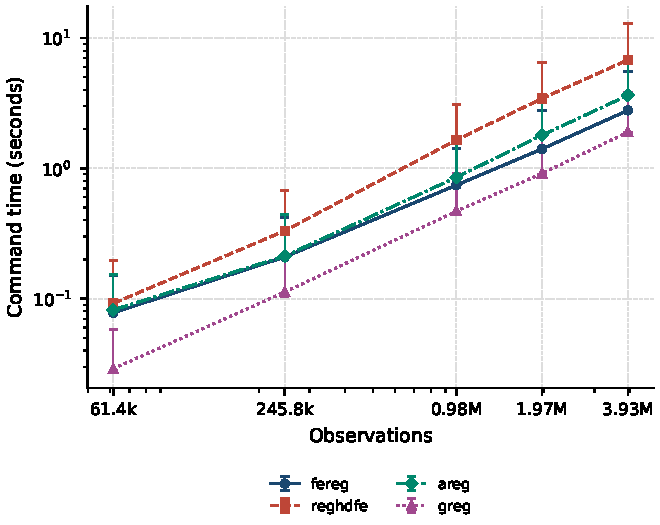
\includegraphics[width=\linewidth]{panels/absolute-ols-stata-one_fe-maximum-seconds.pdf}
\caption{Time by observations}
\end{subfigure}\hfill
\begin{subfigure}[t]{0.485\linewidth}\centering
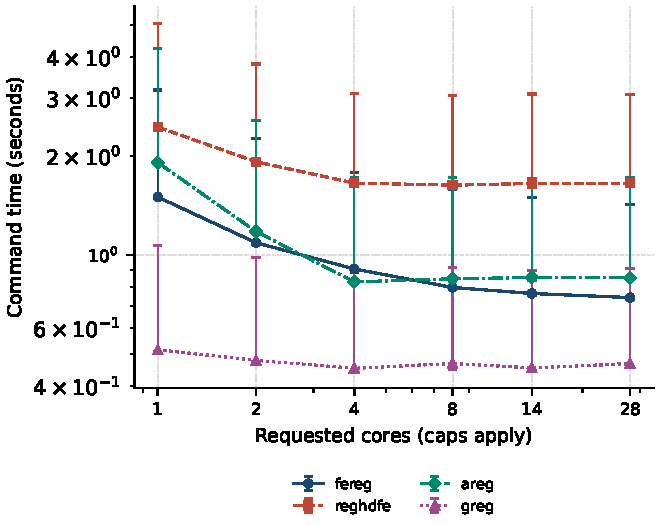
\includegraphics[width=\linewidth]{panels/absolute-ols-stata-one_fe-cores-seconds.pdf}
\caption{Time by requested cores}
\end{subfigure}\par\medskip
\begin{subfigure}[t]{0.485\linewidth}\centering
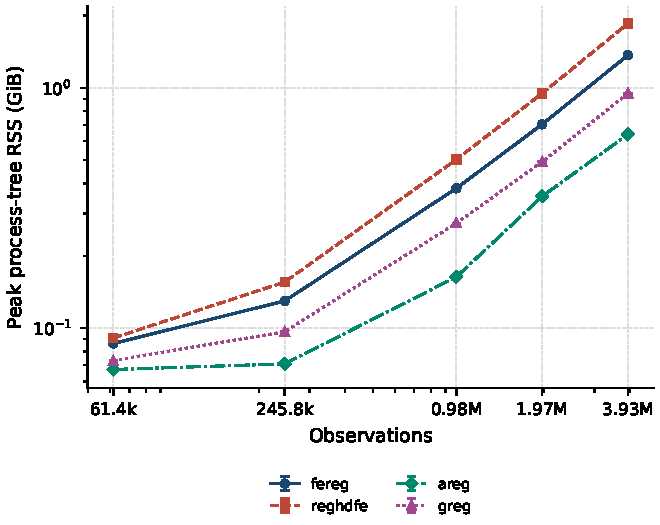
\includegraphics[width=\linewidth]{panels/absolute-ols-stata-one_fe-maximum-peak_rss_gib.pdf}
\caption{RSS by observations}
\end{subfigure}\hfill
\begin{subfigure}[t]{0.485\linewidth}\centering
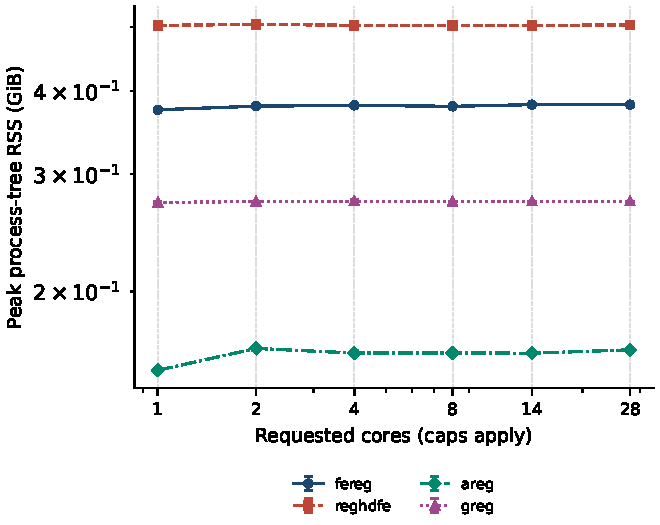
\includegraphics[width=\linewidth]{panels/absolute-ols-stata-one_fe-cores-peak_rss_gib.pdf}
\caption{RSS by requested cores}
\end{subfigure}\par\medskip
\begin{minipage}{0.98\linewidth}\footnotesize Partial campaign. Points require all six valid warm repetitions; bars show IQR, not confidence intervals. Crosses mark missing or unvalidated points. Both axes are logarithmic. Every task reserves 28 cores; Stata-controlled computation is capped at four. OLS IID inference, ten controls. See runs.csv for exclusions.\end{minipage}
\end{figure}\clearpage

\begin{figure}[p]\centering
\caption{OLS One FE: stata, fixed capacity}
\begin{subfigure}[t]{0.485\linewidth}\centering
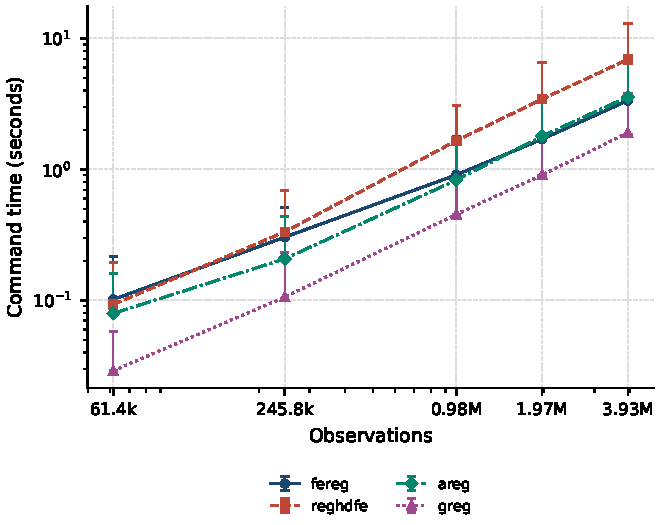
\includegraphics[width=\linewidth]{panels/absolute-ols-stata-one_fe-fixed-seconds.pdf}
\caption{Time by observations}
\end{subfigure}\hfill
\begin{subfigure}[t]{0.485\linewidth}\centering
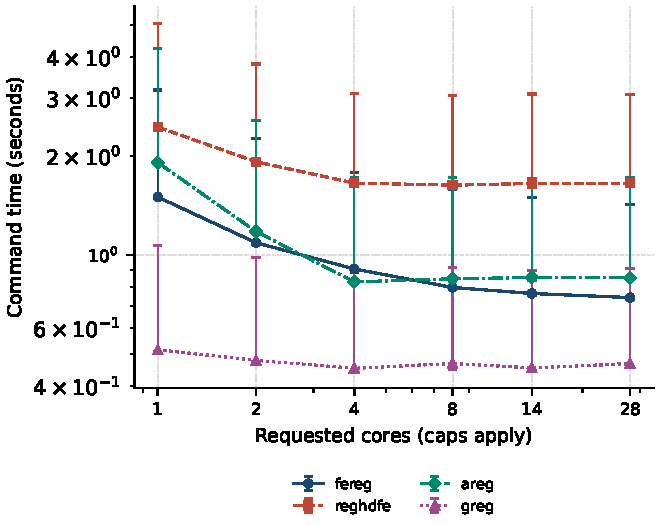
\includegraphics[width=\linewidth]{panels/absolute-ols-stata-one_fe-cores-seconds.pdf}
\caption{Time by requested cores}
\end{subfigure}\par\medskip
\begin{subfigure}[t]{0.485\linewidth}\centering
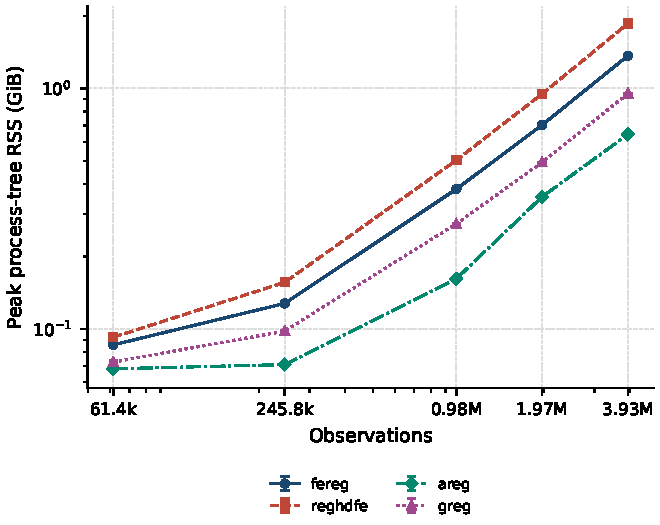
\includegraphics[width=\linewidth]{panels/absolute-ols-stata-one_fe-fixed-peak_rss_gib.pdf}
\caption{RSS by observations}
\end{subfigure}\hfill
\begin{subfigure}[t]{0.485\linewidth}\centering
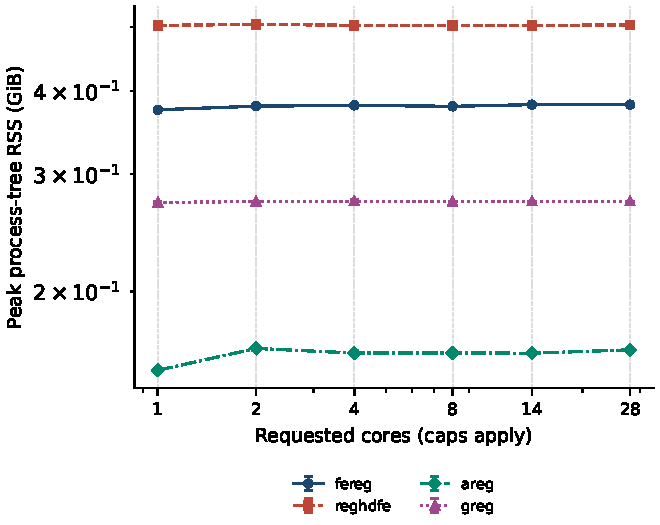
\includegraphics[width=\linewidth]{panels/absolute-ols-stata-one_fe-cores-peak_rss_gib.pdf}
\caption{RSS by requested cores}
\end{subfigure}\par\medskip
\begin{minipage}{0.98\linewidth}\footnotesize Partial campaign. Points require all six valid warm repetitions; bars show IQR, not confidence intervals. Crosses mark missing or unvalidated points. Both axes are logarithmic. Every task reserves 28 cores; Stata-controlled computation is capped at four. OLS IID inference, ten controls. See runs.csv for exclusions.\end{minipage}
\end{figure}\clearpage

\begin{figure}[p]\centering
\caption{OLS Dense two FE: stata, maximum capacity}
\begin{subfigure}[t]{0.485\linewidth}\centering
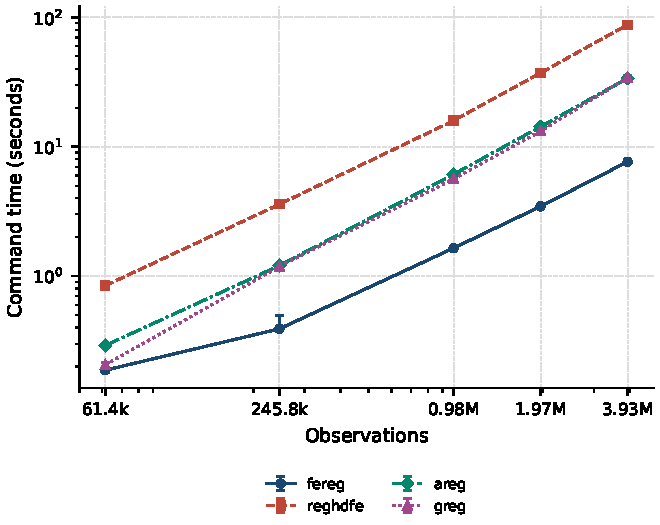
\includegraphics[width=\linewidth]{panels/absolute-ols-stata-two_fe_dense-maximum-seconds.pdf}
\caption{Time by observations}
\end{subfigure}\hfill
\begin{subfigure}[t]{0.485\linewidth}\centering
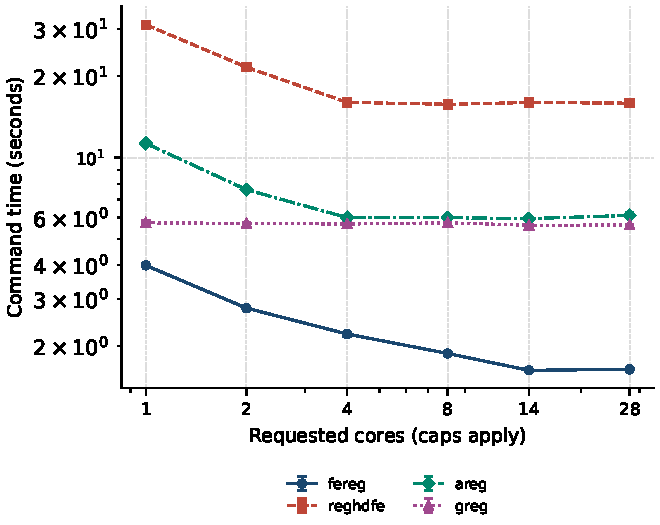
\includegraphics[width=\linewidth]{panels/absolute-ols-stata-two_fe_dense-cores-seconds.pdf}
\caption{Time by requested cores}
\end{subfigure}\par\medskip
\begin{subfigure}[t]{0.485\linewidth}\centering
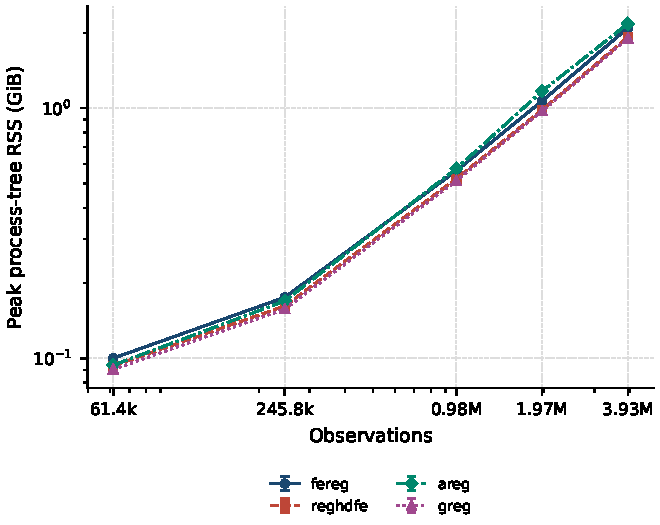
\includegraphics[width=\linewidth]{panels/absolute-ols-stata-two_fe_dense-maximum-peak_rss_gib.pdf}
\caption{RSS by observations}
\end{subfigure}\hfill
\begin{subfigure}[t]{0.485\linewidth}\centering
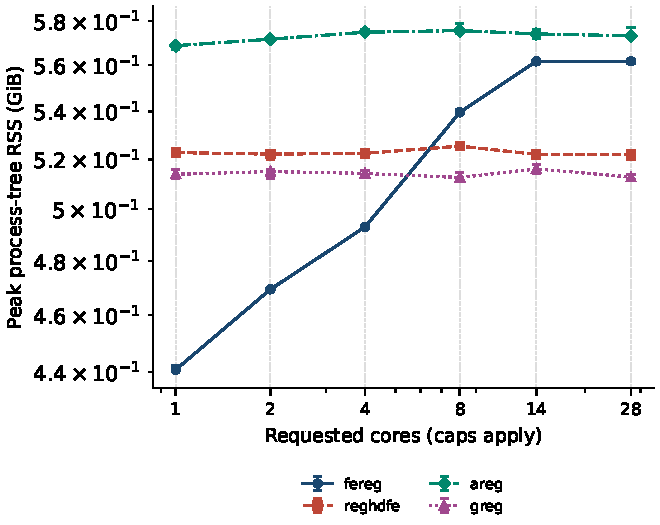
\includegraphics[width=\linewidth]{panels/absolute-ols-stata-two_fe_dense-cores-peak_rss_gib.pdf}
\caption{RSS by requested cores}
\end{subfigure}\par\medskip
\begin{minipage}{0.98\linewidth}\footnotesize Partial campaign. Points require all six valid warm repetitions; bars show IQR, not confidence intervals. Crosses mark missing or unvalidated points. Both axes are logarithmic. Every task reserves 28 cores; Stata-controlled computation is capped at four. OLS IID inference, ten controls. See runs.csv for exclusions.\end{minipage}
\end{figure}\clearpage

\begin{figure}[p]\centering
\caption{OLS Dense two FE: stata, fixed capacity}
\begin{subfigure}[t]{0.485\linewidth}\centering
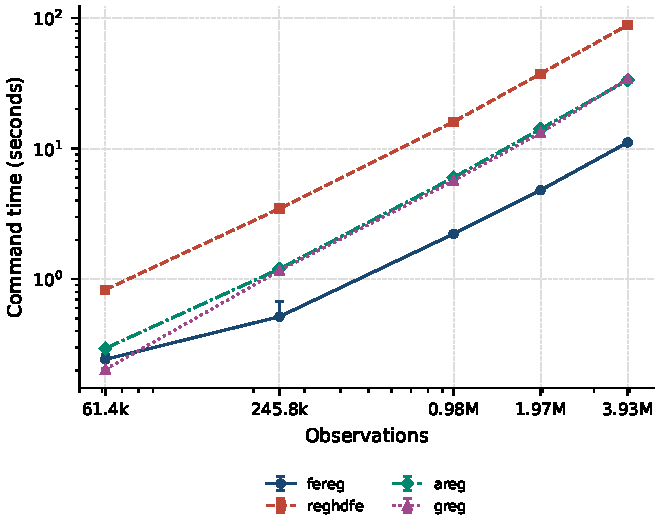
\includegraphics[width=\linewidth]{panels/absolute-ols-stata-two_fe_dense-fixed-seconds.pdf}
\caption{Time by observations}
\end{subfigure}\hfill
\begin{subfigure}[t]{0.485\linewidth}\centering
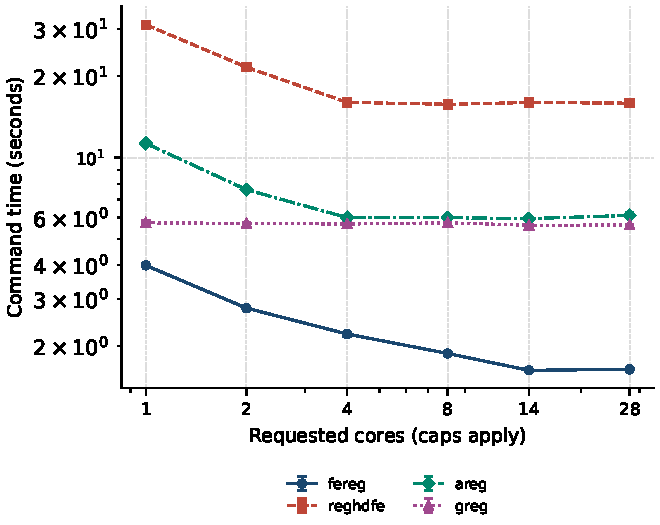
\includegraphics[width=\linewidth]{panels/absolute-ols-stata-two_fe_dense-cores-seconds.pdf}
\caption{Time by requested cores}
\end{subfigure}\par\medskip
\begin{subfigure}[t]{0.485\linewidth}\centering
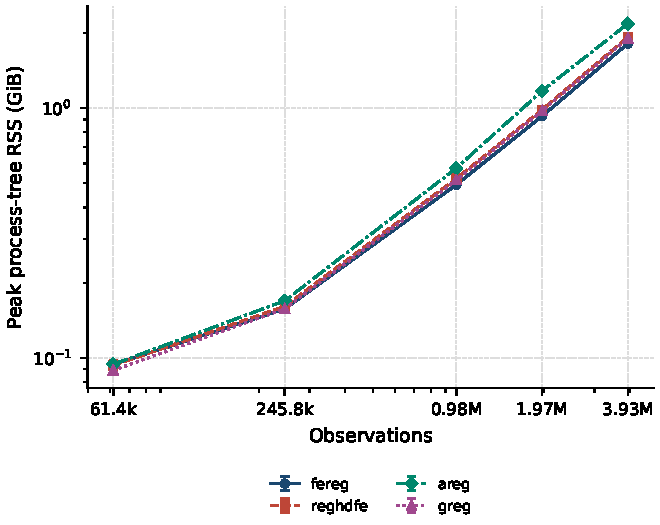
\includegraphics[width=\linewidth]{panels/absolute-ols-stata-two_fe_dense-fixed-peak_rss_gib.pdf}
\caption{RSS by observations}
\end{subfigure}\hfill
\begin{subfigure}[t]{0.485\linewidth}\centering
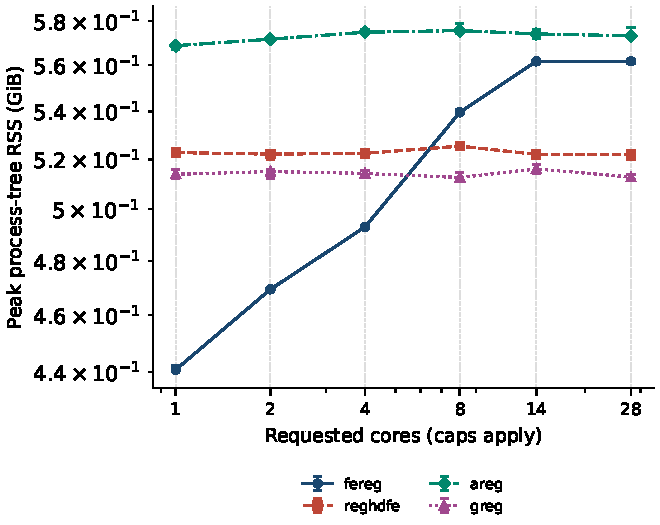
\includegraphics[width=\linewidth]{panels/absolute-ols-stata-two_fe_dense-cores-peak_rss_gib.pdf}
\caption{RSS by requested cores}
\end{subfigure}\par\medskip
\begin{minipage}{0.98\linewidth}\footnotesize Partial campaign. Points require all six valid warm repetitions; bars show IQR, not confidence intervals. Crosses mark missing or unvalidated points. Both axes are logarithmic. Every task reserves 28 cores; Stata-controlled computation is capped at four. OLS IID inference, ten controls. See runs.csv for exclusions.\end{minipage}
\end{figure}\clearpage

\begin{figure}[p]\centering
\caption{OLS Sparse three FE: stata, maximum capacity}
\begin{subfigure}[t]{0.485\linewidth}\centering
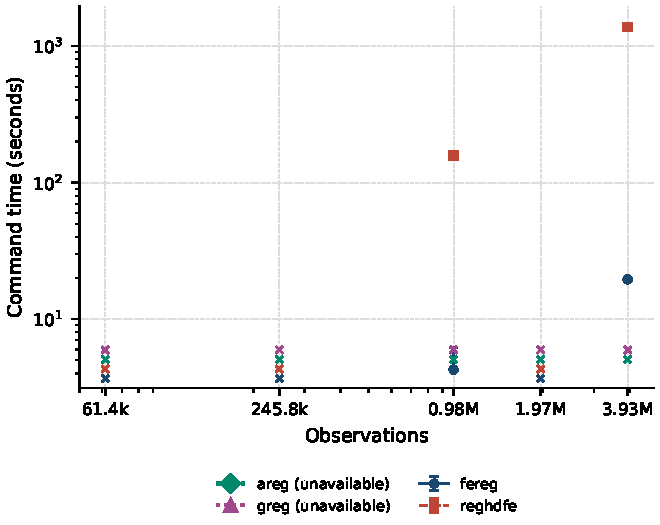
\includegraphics[width=\linewidth]{panels/absolute-ols-stata-three_fe_sparse-maximum-seconds.pdf}
\caption{Time by observations}
\end{subfigure}\hfill
\begin{subfigure}[t]{0.485\linewidth}\centering
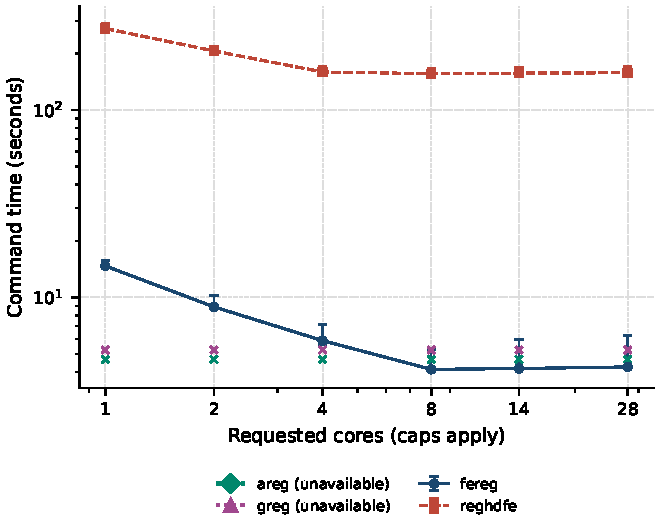
\includegraphics[width=\linewidth]{panels/absolute-ols-stata-three_fe_sparse-cores-seconds.pdf}
\caption{Time by requested cores}
\end{subfigure}\par\medskip
\begin{subfigure}[t]{0.485\linewidth}\centering
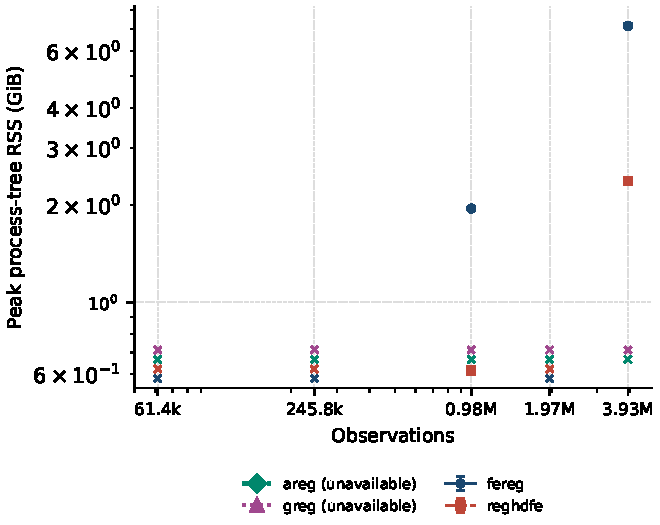
\includegraphics[width=\linewidth]{panels/absolute-ols-stata-three_fe_sparse-maximum-peak_rss_gib.pdf}
\caption{RSS by observations}
\end{subfigure}\hfill
\begin{subfigure}[t]{0.485\linewidth}\centering
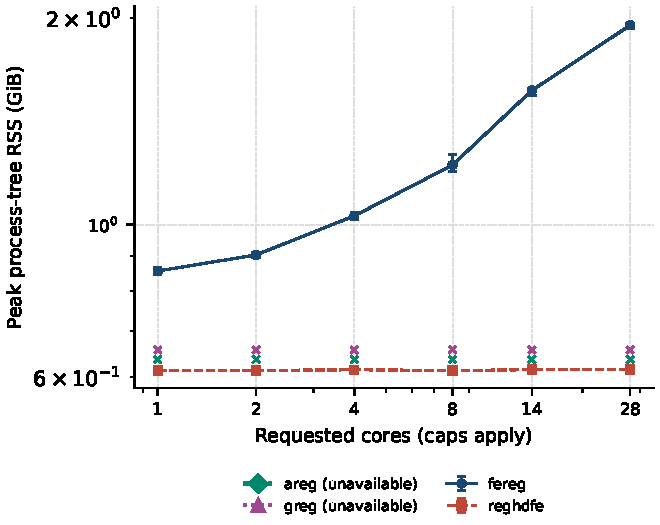
\includegraphics[width=\linewidth]{panels/absolute-ols-stata-three_fe_sparse-cores-peak_rss_gib.pdf}
\caption{RSS by requested cores}
\end{subfigure}\par\medskip
\begin{minipage}{0.98\linewidth}\footnotesize Partial campaign. Points require all six valid warm repetitions; bars show IQR, not confidence intervals. Crosses mark missing or unvalidated points. Both axes are logarithmic. Every task reserves 28 cores; Stata-controlled computation is capped at four. OLS IID inference, ten controls. See runs.csv for exclusions.\end{minipage}
\end{figure}\clearpage

\begin{figure}[p]\centering
\caption{OLS Sparse three FE: stata, fixed capacity}
\begin{subfigure}[t]{0.485\linewidth}\centering
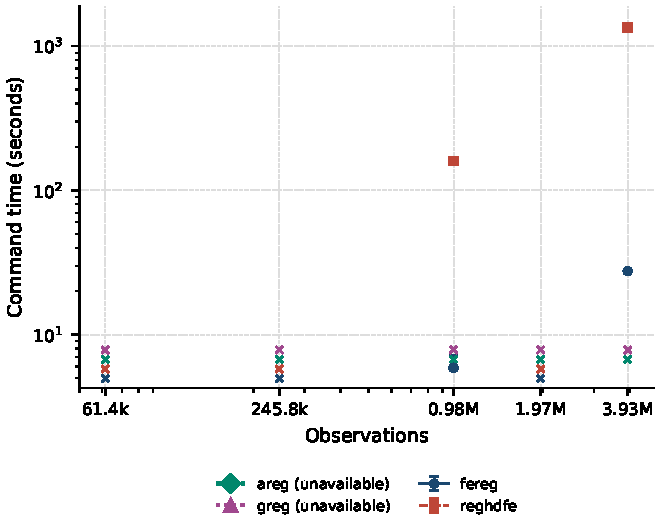
\includegraphics[width=\linewidth]{panels/absolute-ols-stata-three_fe_sparse-fixed-seconds.pdf}
\caption{Time by observations}
\end{subfigure}\hfill
\begin{subfigure}[t]{0.485\linewidth}\centering
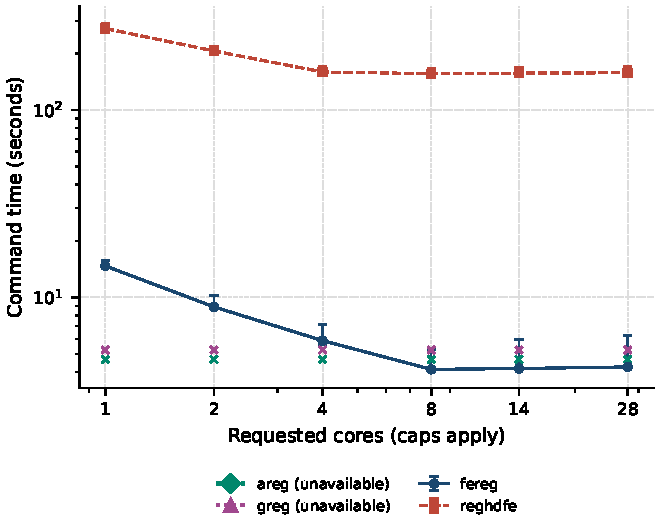
\includegraphics[width=\linewidth]{panels/absolute-ols-stata-three_fe_sparse-cores-seconds.pdf}
\caption{Time by requested cores}
\end{subfigure}\par\medskip
\begin{subfigure}[t]{0.485\linewidth}\centering
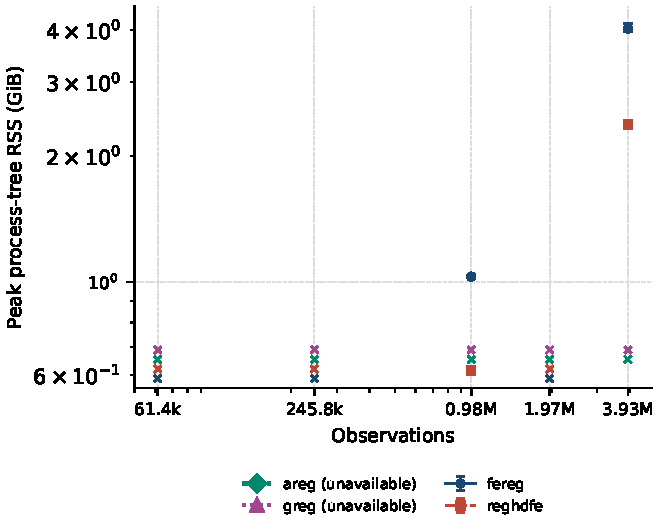
\includegraphics[width=\linewidth]{panels/absolute-ols-stata-three_fe_sparse-fixed-peak_rss_gib.pdf}
\caption{RSS by observations}
\end{subfigure}\hfill
\begin{subfigure}[t]{0.485\linewidth}\centering
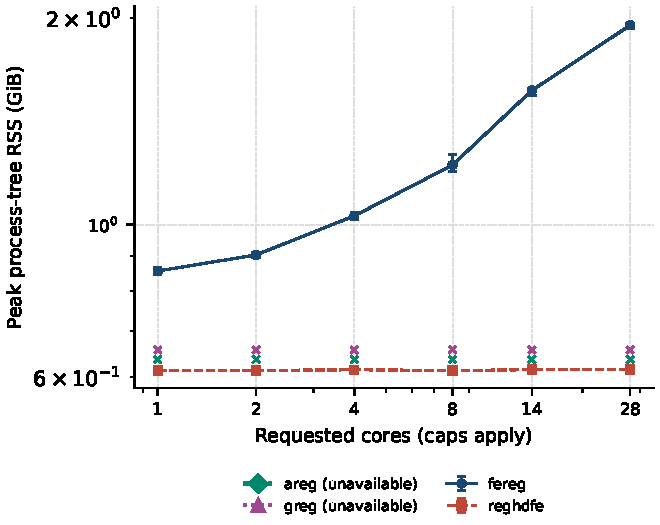
\includegraphics[width=\linewidth]{panels/absolute-ols-stata-three_fe_sparse-cores-peak_rss_gib.pdf}
\caption{RSS by requested cores}
\end{subfigure}\par\medskip
\begin{minipage}{0.98\linewidth}\footnotesize Partial campaign. Points require all six valid warm repetitions; bars show IQR, not confidence intervals. Crosses mark missing or unvalidated points. Both axes are logarithmic. Every task reserves 28 cores; Stata-controlled computation is capped at four. OLS IID inference, ten controls. See runs.csv for exclusions.\end{minipage}
\end{figure}\clearpage

\begin{figure}[p]\centering
\caption{OLS Strong d=2: stata, maximum capacity}
\begin{subfigure}[t]{0.485\linewidth}\centering
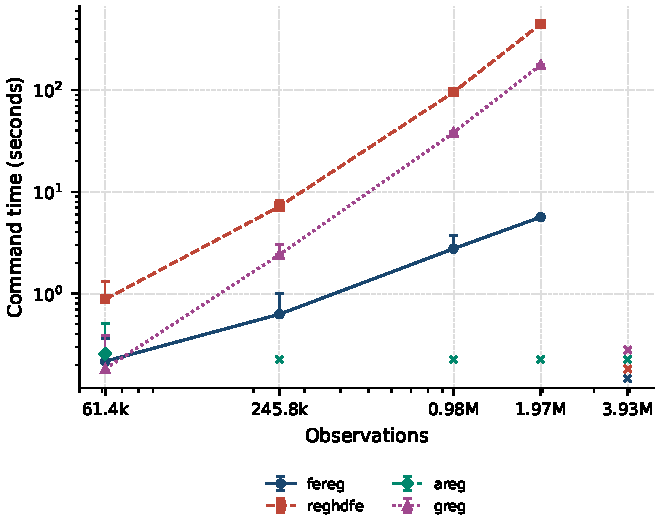
\includegraphics[width=\linewidth]{panels/absolute-ols-stata-strong_d2-maximum-seconds.pdf}
\caption{Time by observations}
\end{subfigure}\hfill
\begin{subfigure}[t]{0.485\linewidth}\centering
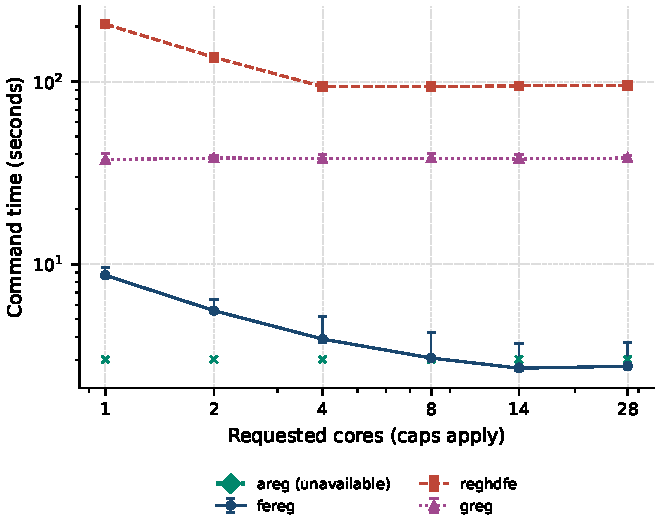
\includegraphics[width=\linewidth]{panels/absolute-ols-stata-strong_d2-cores-seconds.pdf}
\caption{Time by requested cores}
\end{subfigure}\par\medskip
\begin{subfigure}[t]{0.485\linewidth}\centering
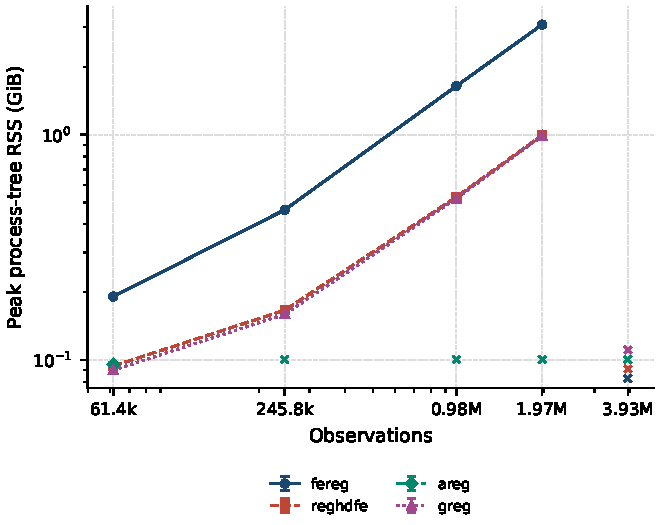
\includegraphics[width=\linewidth]{panels/absolute-ols-stata-strong_d2-maximum-peak_rss_gib.pdf}
\caption{RSS by observations}
\end{subfigure}\hfill
\begin{subfigure}[t]{0.485\linewidth}\centering
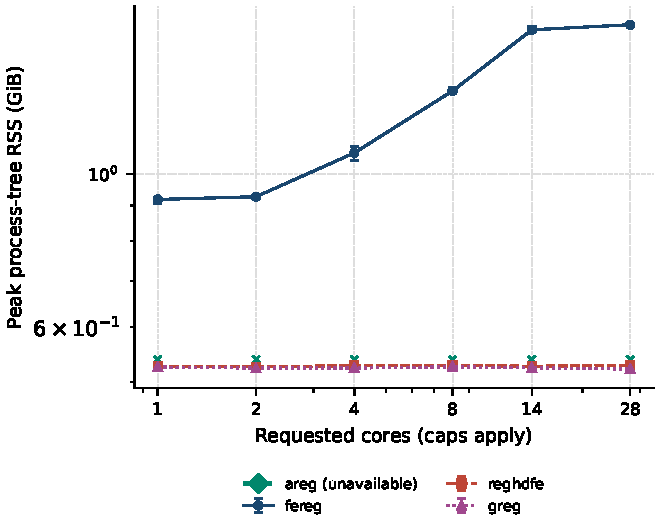
\includegraphics[width=\linewidth]{panels/absolute-ols-stata-strong_d2-cores-peak_rss_gib.pdf}
\caption{RSS by requested cores}
\end{subfigure}\par\medskip
\begin{minipage}{0.98\linewidth}\footnotesize Partial campaign. Points require all six valid warm repetitions; bars show IQR, not confidence intervals. Crosses mark missing or unvalidated points. Both axes are logarithmic. Every task reserves 28 cores; Stata-controlled computation is capped at four. OLS IID inference, ten controls. See runs.csv for exclusions.\end{minipage}
\end{figure}\clearpage

\begin{figure}[p]\centering
\caption{OLS Strong d=2: stata, fixed capacity}
\begin{subfigure}[t]{0.485\linewidth}\centering
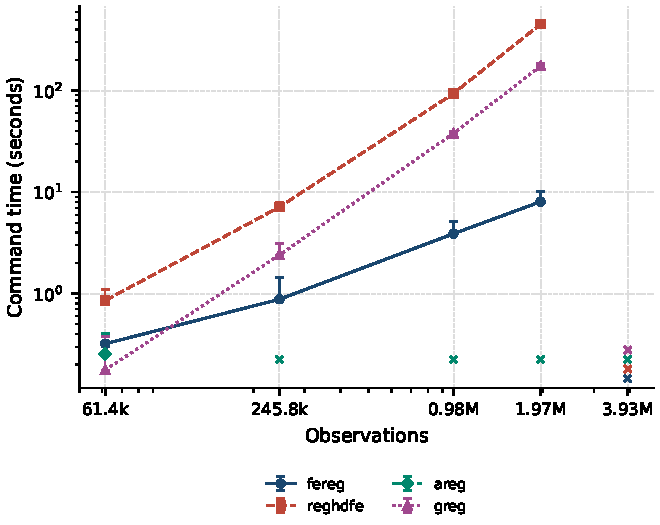
\includegraphics[width=\linewidth]{panels/absolute-ols-stata-strong_d2-fixed-seconds.pdf}
\caption{Time by observations}
\end{subfigure}\hfill
\begin{subfigure}[t]{0.485\linewidth}\centering
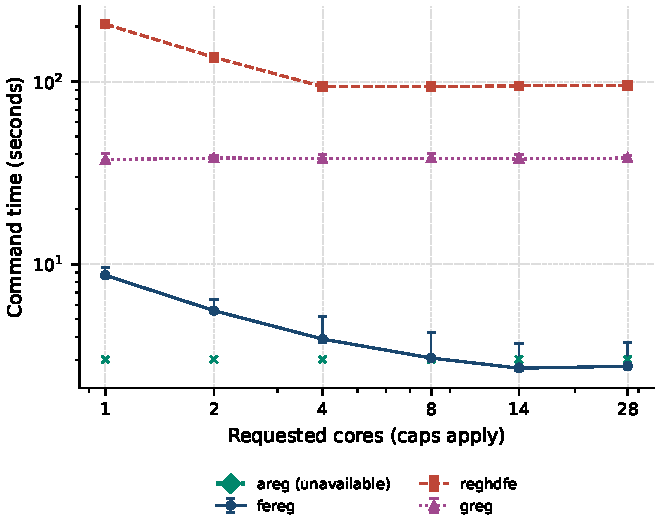
\includegraphics[width=\linewidth]{panels/absolute-ols-stata-strong_d2-cores-seconds.pdf}
\caption{Time by requested cores}
\end{subfigure}\par\medskip
\begin{subfigure}[t]{0.485\linewidth}\centering
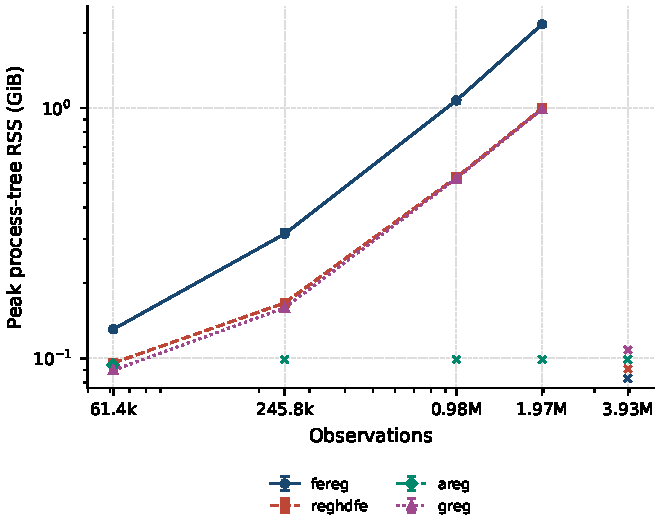
\includegraphics[width=\linewidth]{panels/absolute-ols-stata-strong_d2-fixed-peak_rss_gib.pdf}
\caption{RSS by observations}
\end{subfigure}\hfill
\begin{subfigure}[t]{0.485\linewidth}\centering
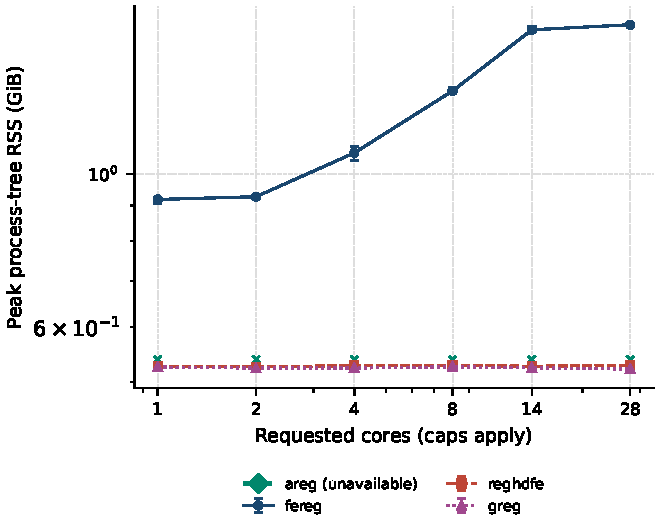
\includegraphics[width=\linewidth]{panels/absolute-ols-stata-strong_d2-cores-peak_rss_gib.pdf}
\caption{RSS by requested cores}
\end{subfigure}\par\medskip
\begin{minipage}{0.98\linewidth}\footnotesize Partial campaign. Points require all six valid warm repetitions; bars show IQR, not confidence intervals. Crosses mark missing or unvalidated points. Both axes are logarithmic. Every task reserves 28 cores; Stata-controlled computation is capped at four. OLS IID inference, ten controls. See runs.csv for exclusions.\end{minipage}
\end{figure}\clearpage

\begin{figure}[p]\centering
\caption{OLS Strong d=3: stata, maximum capacity}
\begin{subfigure}[t]{0.485\linewidth}\centering
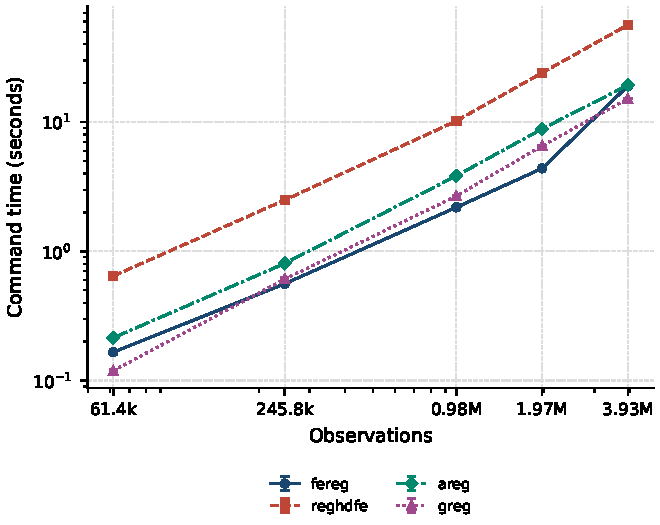
\includegraphics[width=\linewidth]{panels/absolute-ols-stata-strong_d3-maximum-seconds.pdf}
\caption{Time by observations}
\end{subfigure}\hfill
\begin{subfigure}[t]{0.485\linewidth}\centering
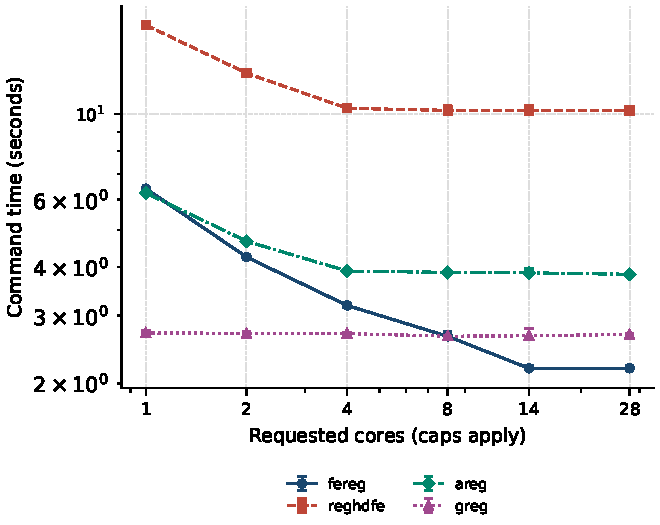
\includegraphics[width=\linewidth]{panels/absolute-ols-stata-strong_d3-cores-seconds.pdf}
\caption{Time by requested cores}
\end{subfigure}\par\medskip
\begin{subfigure}[t]{0.485\linewidth}\centering
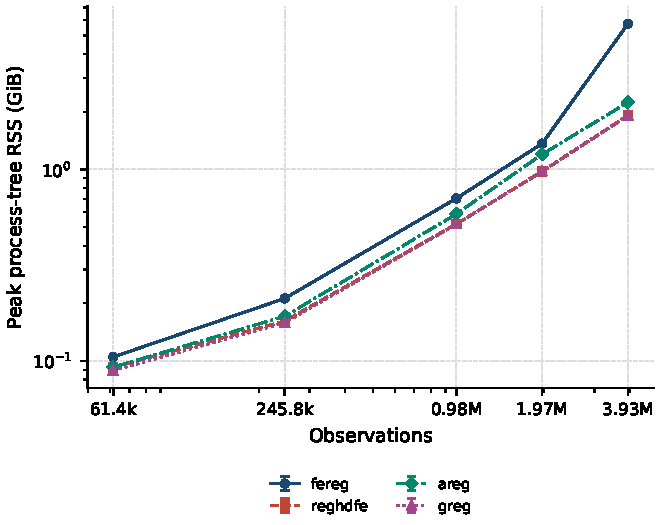
\includegraphics[width=\linewidth]{panels/absolute-ols-stata-strong_d3-maximum-peak_rss_gib.pdf}
\caption{RSS by observations}
\end{subfigure}\hfill
\begin{subfigure}[t]{0.485\linewidth}\centering
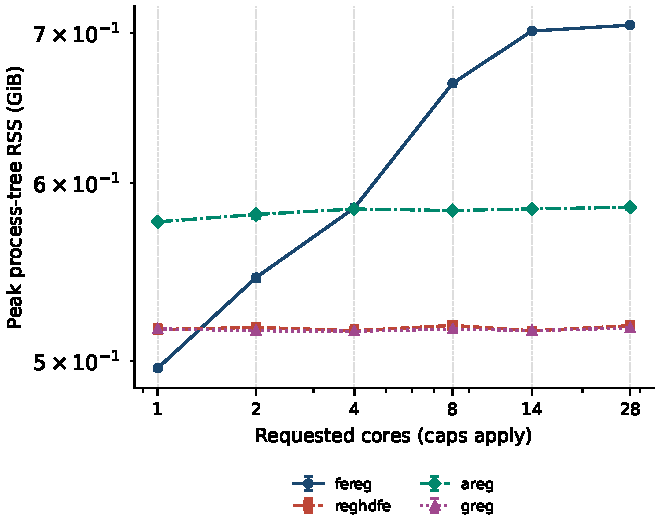
\includegraphics[width=\linewidth]{panels/absolute-ols-stata-strong_d3-cores-peak_rss_gib.pdf}
\caption{RSS by requested cores}
\end{subfigure}\par\medskip
\begin{minipage}{0.98\linewidth}\footnotesize Partial campaign. Points require all six valid warm repetitions; bars show IQR, not confidence intervals. Crosses mark missing or unvalidated points. Both axes are logarithmic. Every task reserves 28 cores; Stata-controlled computation is capped at four. OLS IID inference, ten controls. See runs.csv for exclusions.\end{minipage}
\end{figure}\clearpage

\begin{figure}[p]\centering
\caption{OLS Strong d=3: stata, fixed capacity}
\begin{subfigure}[t]{0.485\linewidth}\centering
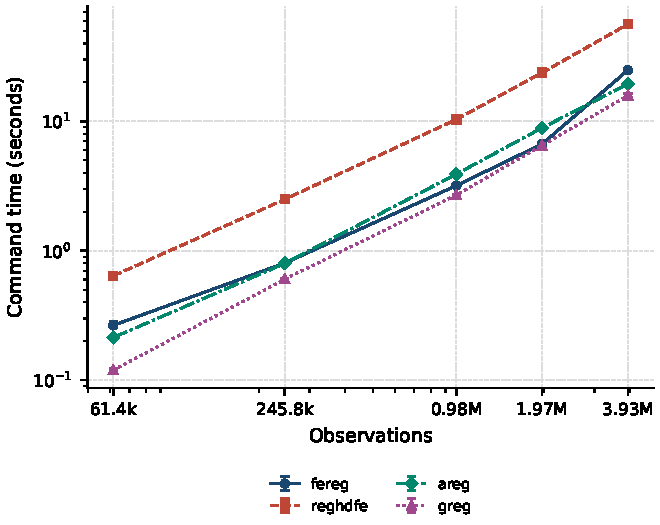
\includegraphics[width=\linewidth]{panels/absolute-ols-stata-strong_d3-fixed-seconds.pdf}
\caption{Time by observations}
\end{subfigure}\hfill
\begin{subfigure}[t]{0.485\linewidth}\centering
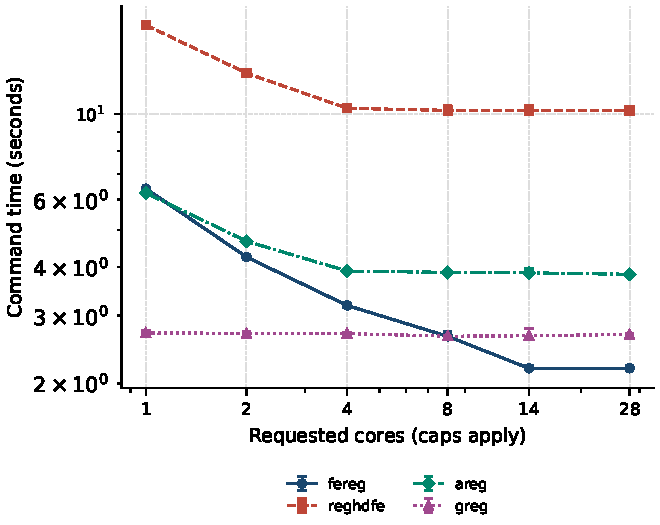
\includegraphics[width=\linewidth]{panels/absolute-ols-stata-strong_d3-cores-seconds.pdf}
\caption{Time by requested cores}
\end{subfigure}\par\medskip
\begin{subfigure}[t]{0.485\linewidth}\centering
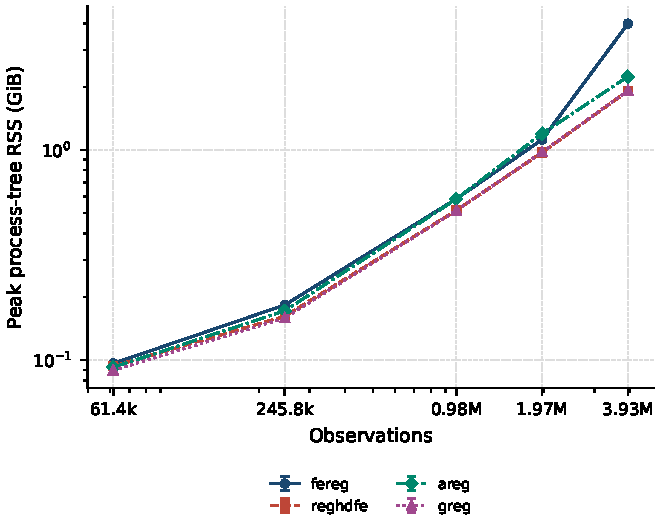
\includegraphics[width=\linewidth]{panels/absolute-ols-stata-strong_d3-fixed-peak_rss_gib.pdf}
\caption{RSS by observations}
\end{subfigure}\hfill
\begin{subfigure}[t]{0.485\linewidth}\centering
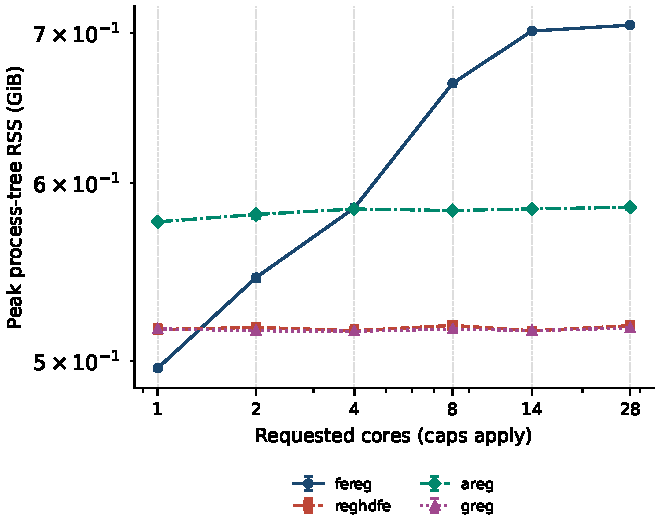
\includegraphics[width=\linewidth]{panels/absolute-ols-stata-strong_d3-cores-peak_rss_gib.pdf}
\caption{RSS by requested cores}
\end{subfigure}\par\medskip
\begin{minipage}{0.98\linewidth}\footnotesize Partial campaign. Points require all six valid warm repetitions; bars show IQR, not confidence intervals. Crosses mark missing or unvalidated points. Both axes are logarithmic. Every task reserves 28 cores; Stata-controlled computation is capped at four. OLS IID inference, ten controls. See runs.csv for exclusions.\end{minipage}
\end{figure}\clearpage

\begin{figure}[p]\centering
\caption{OLS Strong d=6: stata, maximum capacity}
\begin{subfigure}[t]{0.485\linewidth}\centering
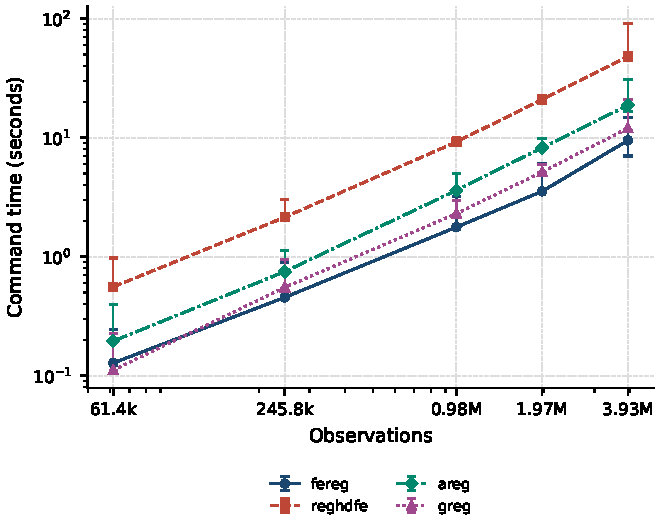
\includegraphics[width=\linewidth]{panels/absolute-ols-stata-strong_d6-maximum-seconds.pdf}
\caption{Time by observations}
\end{subfigure}\hfill
\begin{subfigure}[t]{0.485\linewidth}\centering
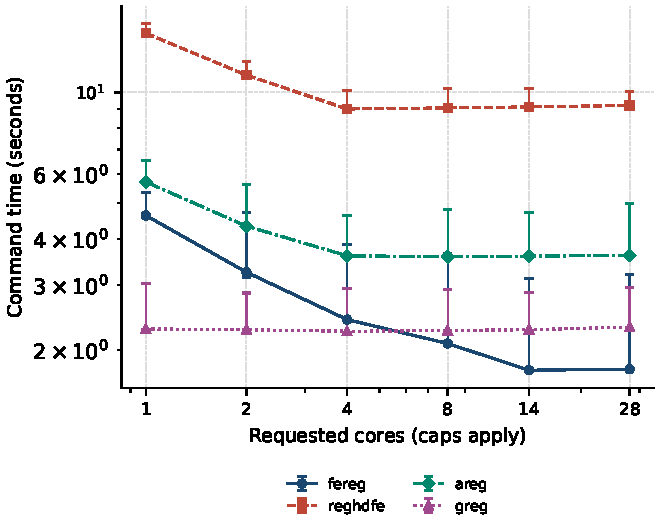
\includegraphics[width=\linewidth]{panels/absolute-ols-stata-strong_d6-cores-seconds.pdf}
\caption{Time by requested cores}
\end{subfigure}\par\medskip
\begin{subfigure}[t]{0.485\linewidth}\centering
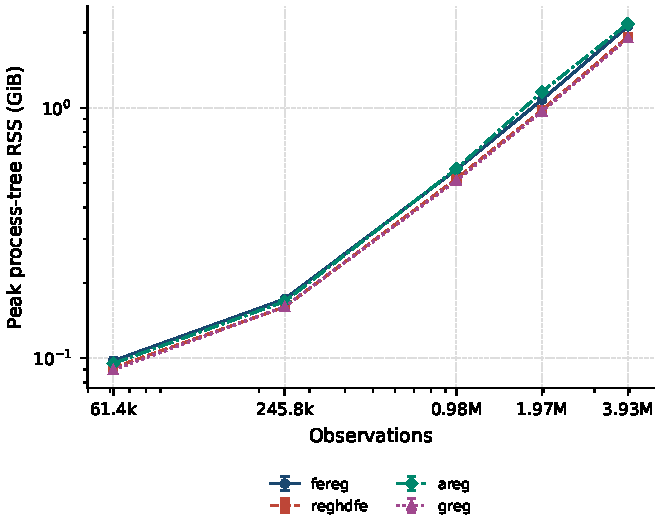
\includegraphics[width=\linewidth]{panels/absolute-ols-stata-strong_d6-maximum-peak_rss_gib.pdf}
\caption{RSS by observations}
\end{subfigure}\hfill
\begin{subfigure}[t]{0.485\linewidth}\centering
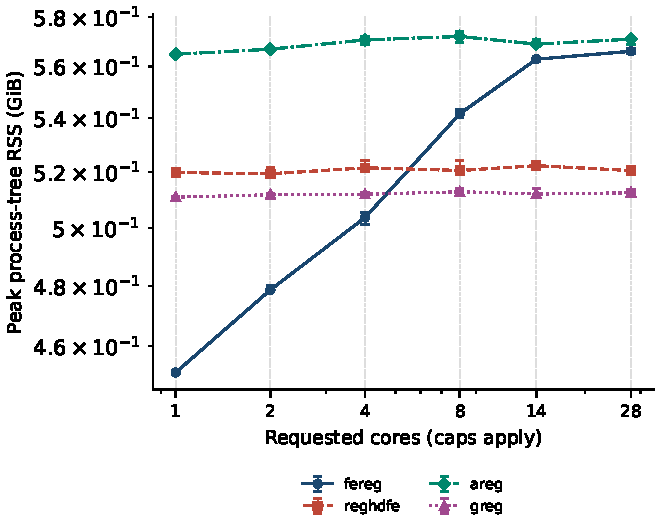
\includegraphics[width=\linewidth]{panels/absolute-ols-stata-strong_d6-cores-peak_rss_gib.pdf}
\caption{RSS by requested cores}
\end{subfigure}\par\medskip
\begin{minipage}{0.98\linewidth}\footnotesize Partial campaign. Points require all six valid warm repetitions; bars show IQR, not confidence intervals. Crosses mark missing or unvalidated points. Both axes are logarithmic. Every task reserves 28 cores; Stata-controlled computation is capped at four. OLS IID inference, ten controls. See runs.csv for exclusions.\end{minipage}
\end{figure}\clearpage

\begin{figure}[p]\centering
\caption{OLS Strong d=6: stata, fixed capacity}
\begin{subfigure}[t]{0.485\linewidth}\centering
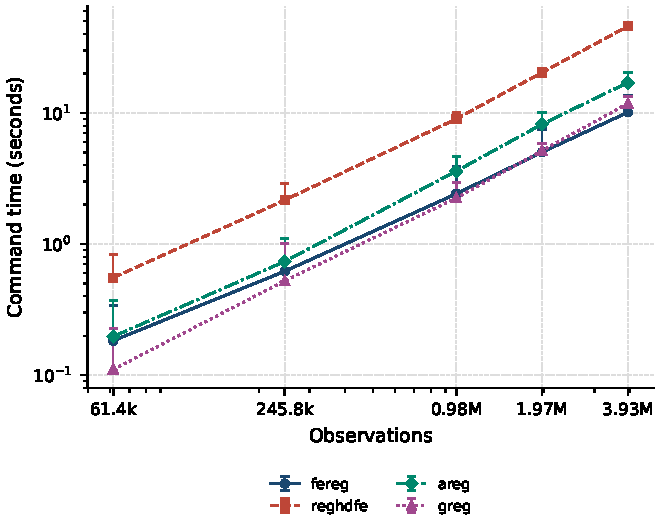
\includegraphics[width=\linewidth]{panels/absolute-ols-stata-strong_d6-fixed-seconds.pdf}
\caption{Time by observations}
\end{subfigure}\hfill
\begin{subfigure}[t]{0.485\linewidth}\centering
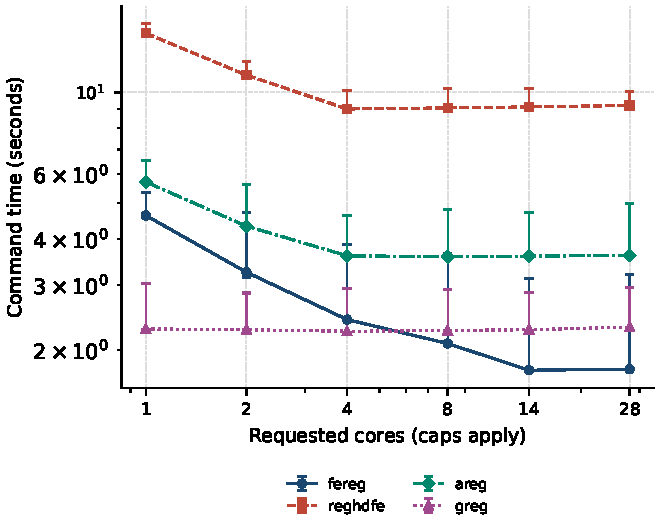
\includegraphics[width=\linewidth]{panels/absolute-ols-stata-strong_d6-cores-seconds.pdf}
\caption{Time by requested cores}
\end{subfigure}\par\medskip
\begin{subfigure}[t]{0.485\linewidth}\centering
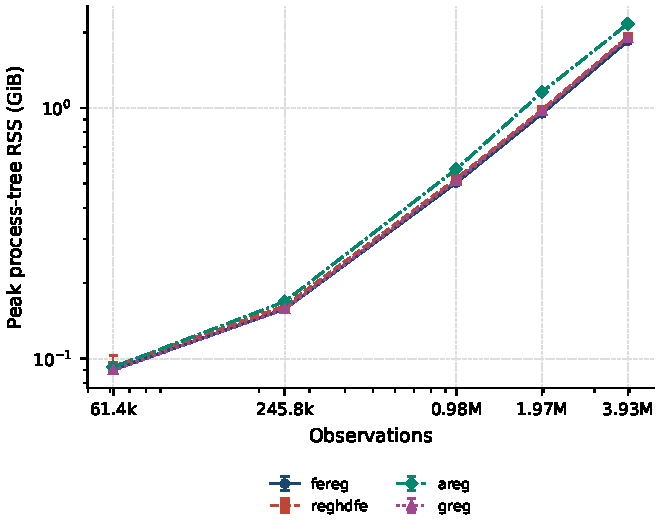
\includegraphics[width=\linewidth]{panels/absolute-ols-stata-strong_d6-fixed-peak_rss_gib.pdf}
\caption{RSS by observations}
\end{subfigure}\hfill
\begin{subfigure}[t]{0.485\linewidth}\centering
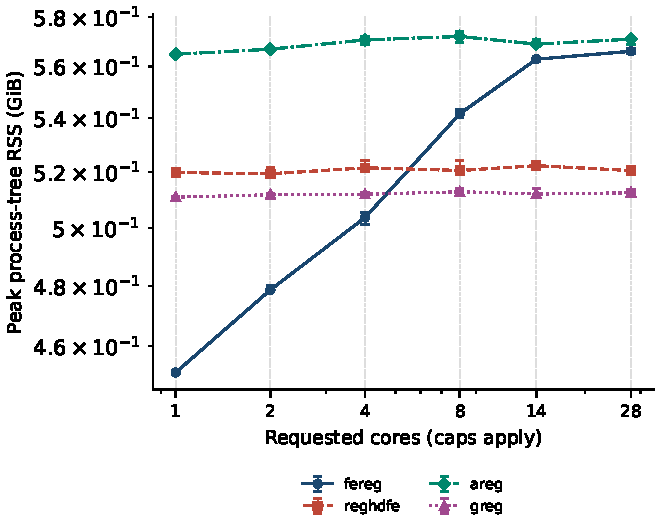
\includegraphics[width=\linewidth]{panels/absolute-ols-stata-strong_d6-cores-peak_rss_gib.pdf}
\caption{RSS by requested cores}
\end{subfigure}\par\medskip
\begin{minipage}{0.98\linewidth}\footnotesize Partial campaign. Points require all six valid warm repetitions; bars show IQR, not confidence intervals. Crosses mark missing or unvalidated points. Both axes are logarithmic. Every task reserves 28 cores; Stata-controlled computation is capped at four. OLS IID inference, ten controls. See runs.csv for exclusions.\end{minipage}
\end{figure}\clearpage

\begin{figure}[p]\centering
\caption{OLS One FE: expanded, maximum capacity}
\begin{subfigure}[t]{0.485\linewidth}\centering
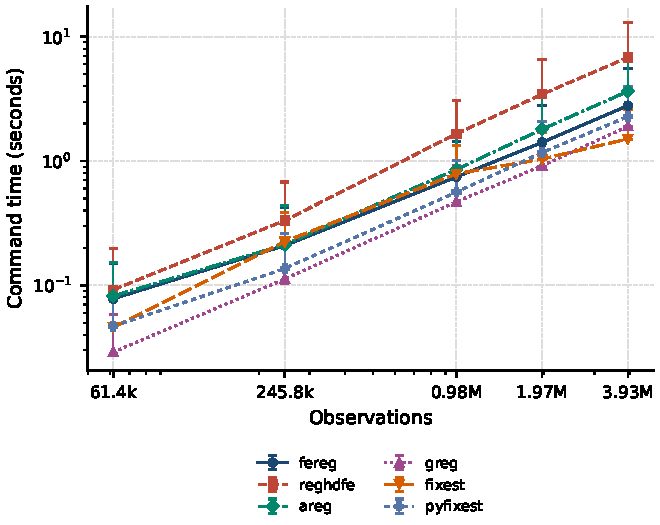
\includegraphics[width=\linewidth]{panels/absolute-ols-expanded-one_fe-maximum-seconds.pdf}
\caption{Time by observations}
\end{subfigure}\hfill
\begin{subfigure}[t]{0.485\linewidth}\centering
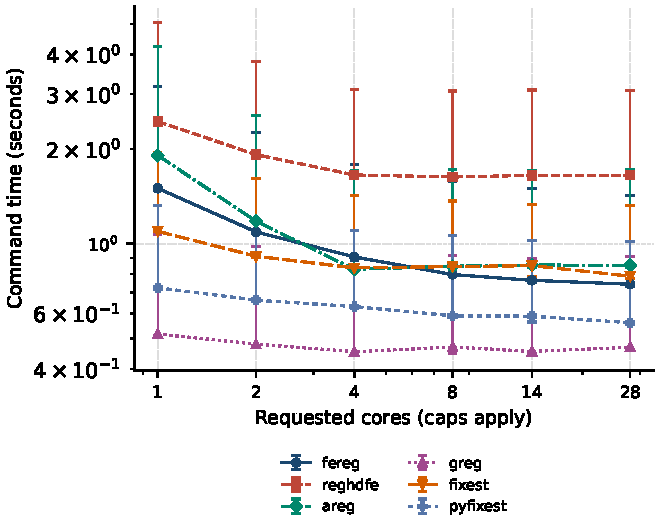
\includegraphics[width=\linewidth]{panels/absolute-ols-expanded-one_fe-cores-seconds.pdf}
\caption{Time by requested cores}
\end{subfigure}\par\medskip
\begin{subfigure}[t]{0.485\linewidth}\centering
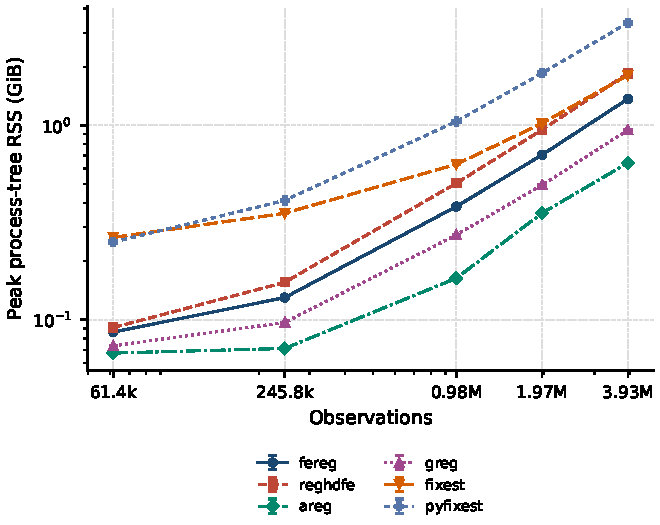
\includegraphics[width=\linewidth]{panels/absolute-ols-expanded-one_fe-maximum-peak_rss_gib.pdf}
\caption{RSS by observations}
\end{subfigure}\hfill
\begin{subfigure}[t]{0.485\linewidth}\centering
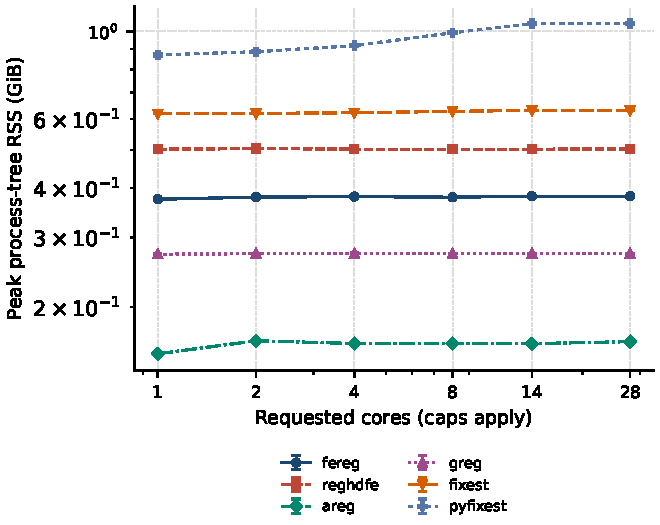
\includegraphics[width=\linewidth]{panels/absolute-ols-expanded-one_fe-cores-peak_rss_gib.pdf}
\caption{RSS by requested cores}
\end{subfigure}\par\medskip
\begin{minipage}{0.98\linewidth}\footnotesize Partial campaign. Points require all six valid warm repetitions; bars show IQR, not confidence intervals. Crosses mark missing or unvalidated points. Both axes are logarithmic. Every task reserves 28 cores; Stata-controlled computation is capped at four. OLS IID inference, ten controls. See runs.csv for exclusions.\end{minipage}
\end{figure}\clearpage

\begin{figure}[p]\centering
\caption{OLS One FE: expanded, fixed capacity}
\begin{subfigure}[t]{0.485\linewidth}\centering
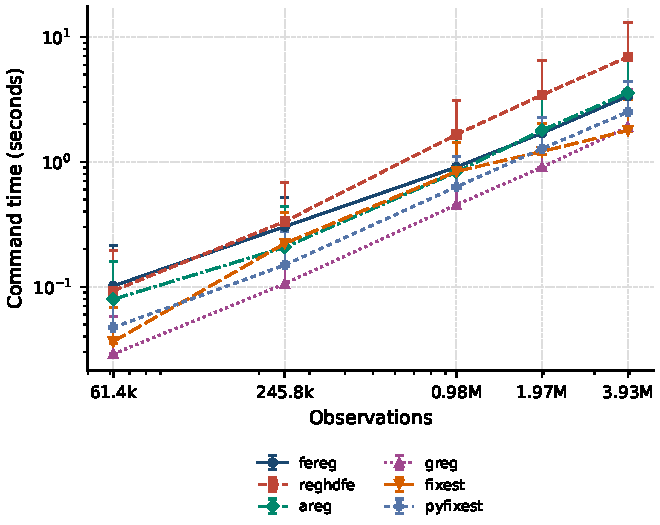
\includegraphics[width=\linewidth]{panels/absolute-ols-expanded-one_fe-fixed-seconds.pdf}
\caption{Time by observations}
\end{subfigure}\hfill
\begin{subfigure}[t]{0.485\linewidth}\centering
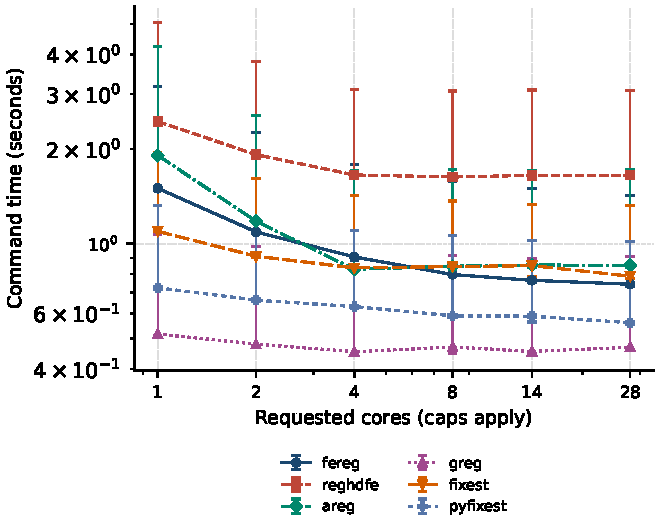
\includegraphics[width=\linewidth]{panels/absolute-ols-expanded-one_fe-cores-seconds.pdf}
\caption{Time by requested cores}
\end{subfigure}\par\medskip
\begin{subfigure}[t]{0.485\linewidth}\centering
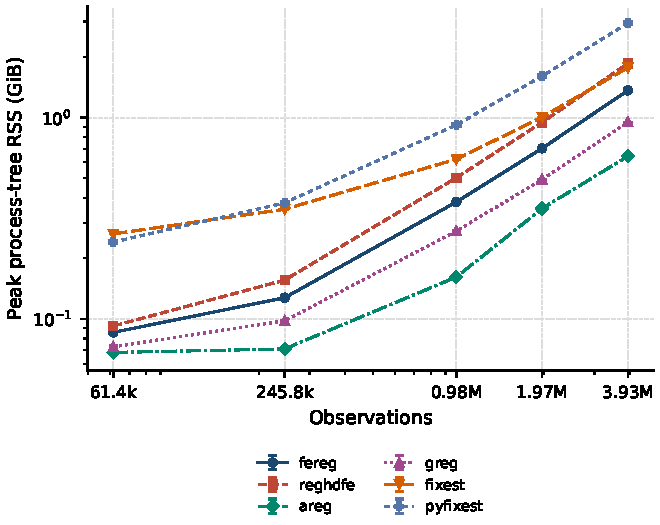
\includegraphics[width=\linewidth]{panels/absolute-ols-expanded-one_fe-fixed-peak_rss_gib.pdf}
\caption{RSS by observations}
\end{subfigure}\hfill
\begin{subfigure}[t]{0.485\linewidth}\centering
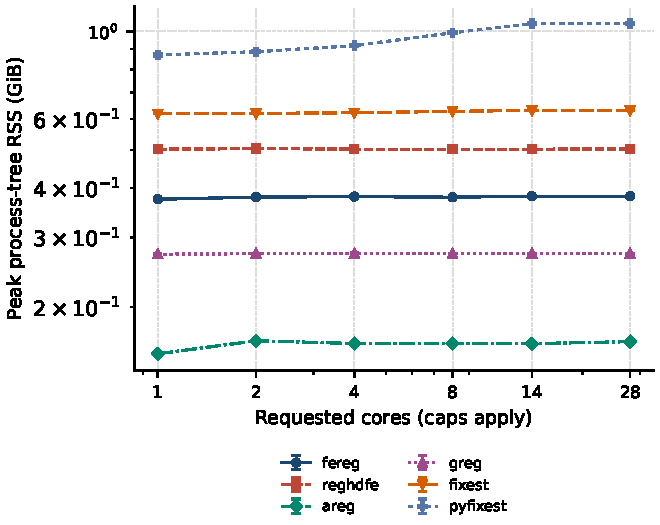
\includegraphics[width=\linewidth]{panels/absolute-ols-expanded-one_fe-cores-peak_rss_gib.pdf}
\caption{RSS by requested cores}
\end{subfigure}\par\medskip
\begin{minipage}{0.98\linewidth}\footnotesize Partial campaign. Points require all six valid warm repetitions; bars show IQR, not confidence intervals. Crosses mark missing or unvalidated points. Both axes are logarithmic. Every task reserves 28 cores; Stata-controlled computation is capped at four. OLS IID inference, ten controls. See runs.csv for exclusions.\end{minipage}
\end{figure}\clearpage

\begin{figure}[p]\centering
\caption{OLS Dense two FE: expanded, maximum capacity}
\begin{subfigure}[t]{0.485\linewidth}\centering
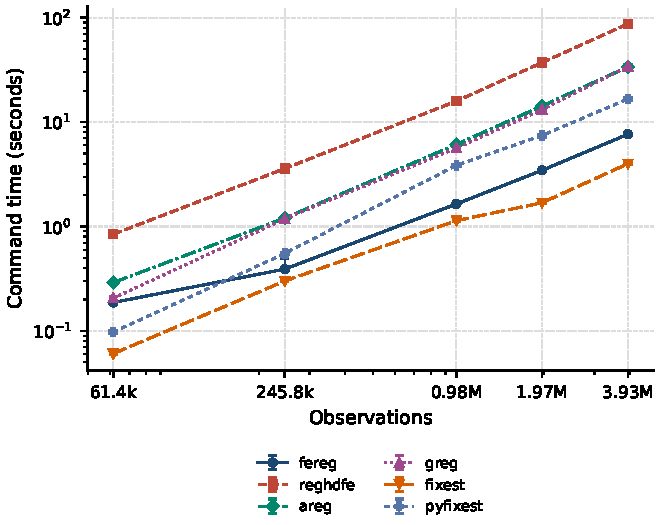
\includegraphics[width=\linewidth]{panels/absolute-ols-expanded-two_fe_dense-maximum-seconds.pdf}
\caption{Time by observations}
\end{subfigure}\hfill
\begin{subfigure}[t]{0.485\linewidth}\centering
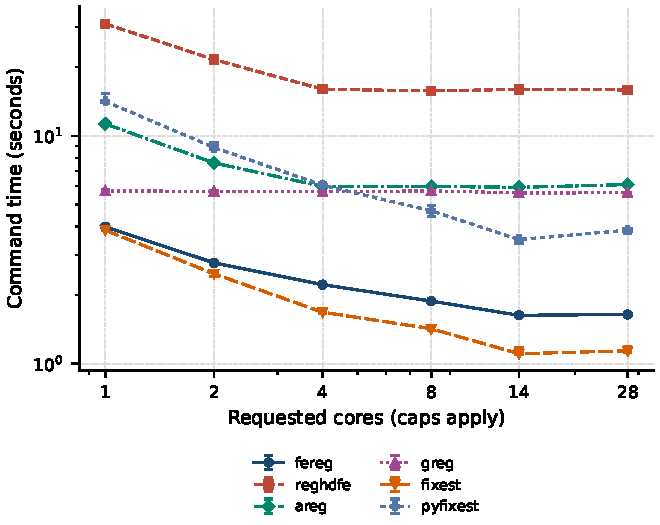
\includegraphics[width=\linewidth]{panels/absolute-ols-expanded-two_fe_dense-cores-seconds.pdf}
\caption{Time by requested cores}
\end{subfigure}\par\medskip
\begin{subfigure}[t]{0.485\linewidth}\centering
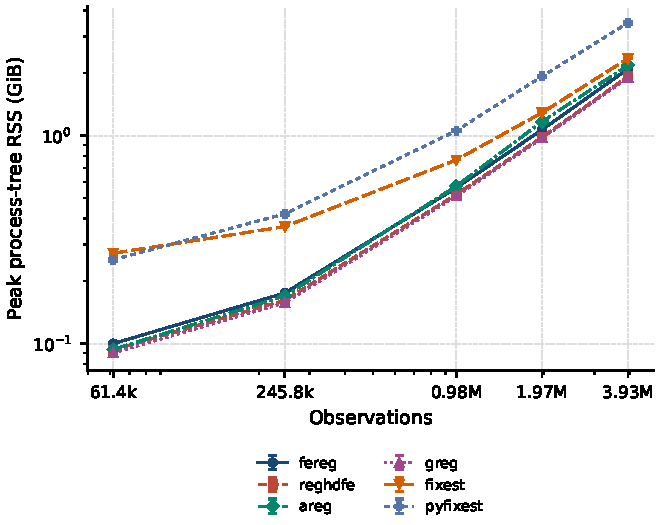
\includegraphics[width=\linewidth]{panels/absolute-ols-expanded-two_fe_dense-maximum-peak_rss_gib.pdf}
\caption{RSS by observations}
\end{subfigure}\hfill
\begin{subfigure}[t]{0.485\linewidth}\centering
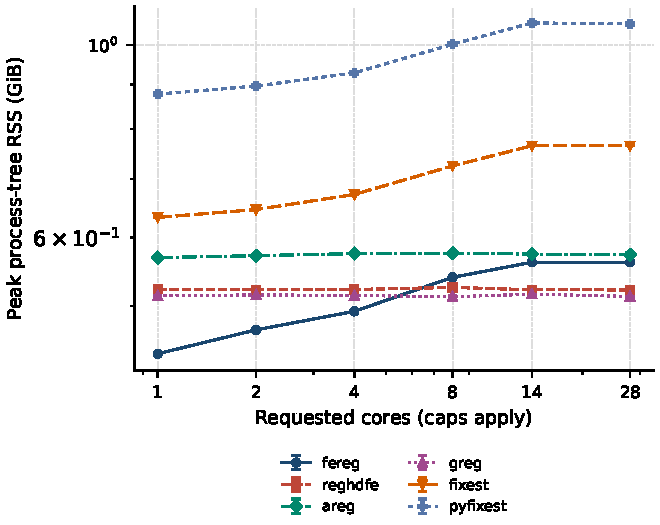
\includegraphics[width=\linewidth]{panels/absolute-ols-expanded-two_fe_dense-cores-peak_rss_gib.pdf}
\caption{RSS by requested cores}
\end{subfigure}\par\medskip
\begin{minipage}{0.98\linewidth}\footnotesize Partial campaign. Points require all six valid warm repetitions; bars show IQR, not confidence intervals. Crosses mark missing or unvalidated points. Both axes are logarithmic. Every task reserves 28 cores; Stata-controlled computation is capped at four. OLS IID inference, ten controls. See runs.csv for exclusions.\end{minipage}
\end{figure}\clearpage

\begin{figure}[p]\centering
\caption{OLS Dense two FE: expanded, fixed capacity}
\begin{subfigure}[t]{0.485\linewidth}\centering
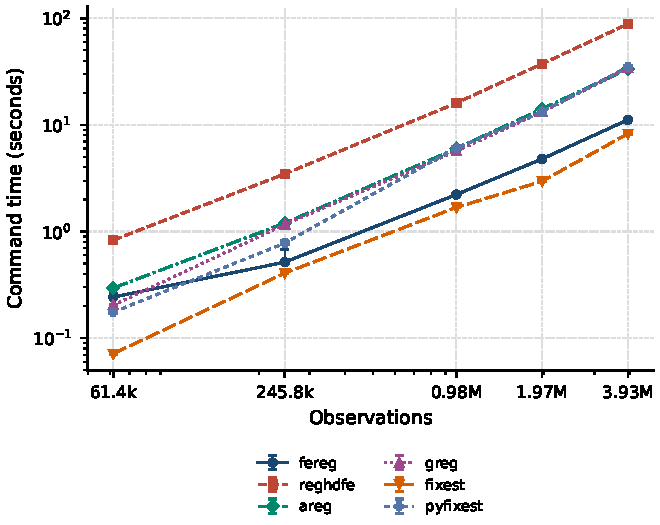
\includegraphics[width=\linewidth]{panels/absolute-ols-expanded-two_fe_dense-fixed-seconds.pdf}
\caption{Time by observations}
\end{subfigure}\hfill
\begin{subfigure}[t]{0.485\linewidth}\centering
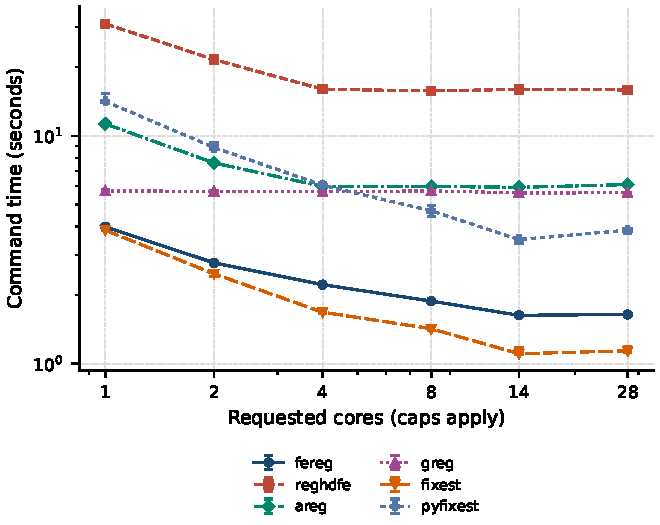
\includegraphics[width=\linewidth]{panels/absolute-ols-expanded-two_fe_dense-cores-seconds.pdf}
\caption{Time by requested cores}
\end{subfigure}\par\medskip
\begin{subfigure}[t]{0.485\linewidth}\centering
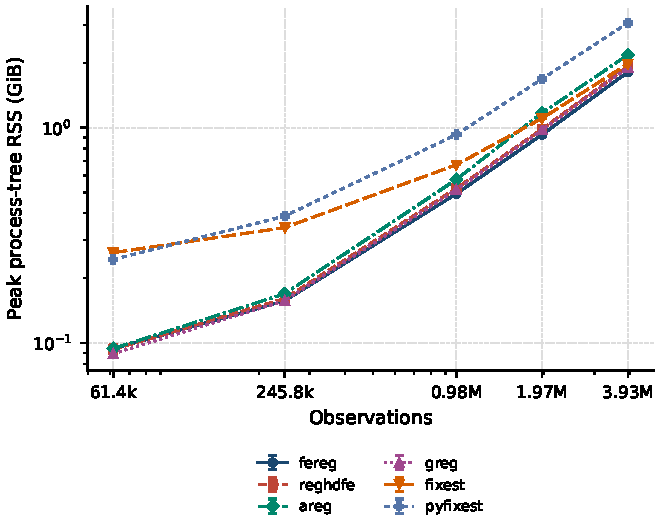
\includegraphics[width=\linewidth]{panels/absolute-ols-expanded-two_fe_dense-fixed-peak_rss_gib.pdf}
\caption{RSS by observations}
\end{subfigure}\hfill
\begin{subfigure}[t]{0.485\linewidth}\centering
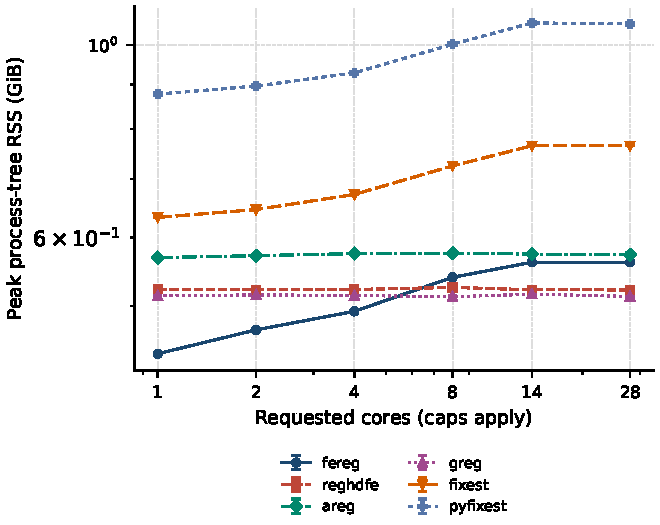
\includegraphics[width=\linewidth]{panels/absolute-ols-expanded-two_fe_dense-cores-peak_rss_gib.pdf}
\caption{RSS by requested cores}
\end{subfigure}\par\medskip
\begin{minipage}{0.98\linewidth}\footnotesize Partial campaign. Points require all six valid warm repetitions; bars show IQR, not confidence intervals. Crosses mark missing or unvalidated points. Both axes are logarithmic. Every task reserves 28 cores; Stata-controlled computation is capped at four. OLS IID inference, ten controls. See runs.csv for exclusions.\end{minipage}
\end{figure}\clearpage

\begin{figure}[p]\centering
\caption{OLS Sparse three FE: expanded, maximum capacity}
\begin{subfigure}[t]{0.485\linewidth}\centering
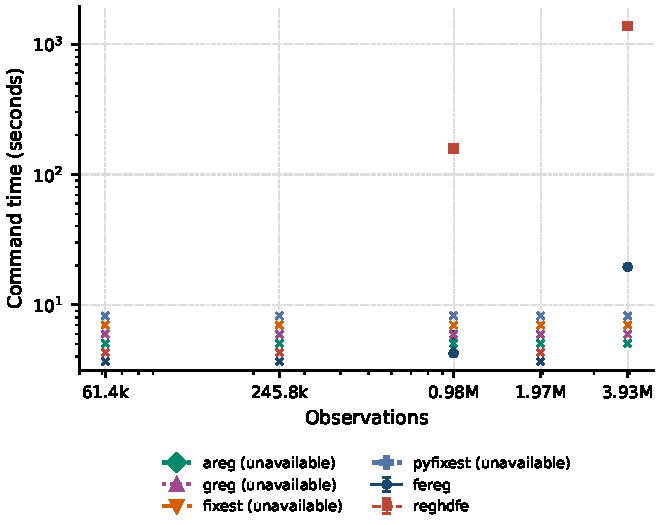
\includegraphics[width=\linewidth]{panels/absolute-ols-expanded-three_fe_sparse-maximum-seconds.pdf}
\caption{Time by observations}
\end{subfigure}\hfill
\begin{subfigure}[t]{0.485\linewidth}\centering
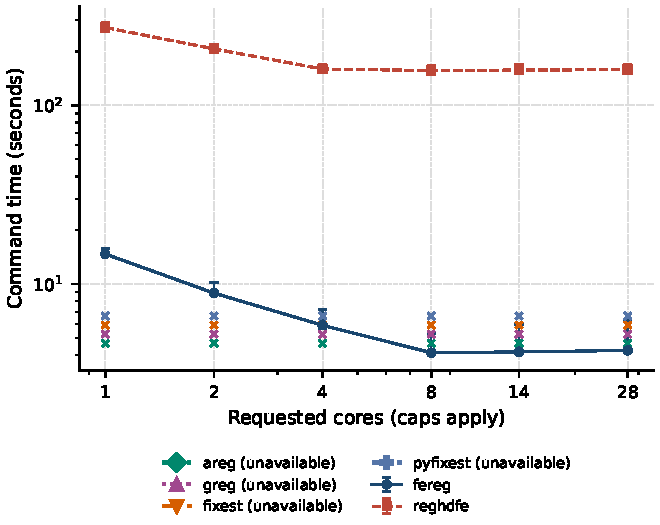
\includegraphics[width=\linewidth]{panels/absolute-ols-expanded-three_fe_sparse-cores-seconds.pdf}
\caption{Time by requested cores}
\end{subfigure}\par\medskip
\begin{subfigure}[t]{0.485\linewidth}\centering
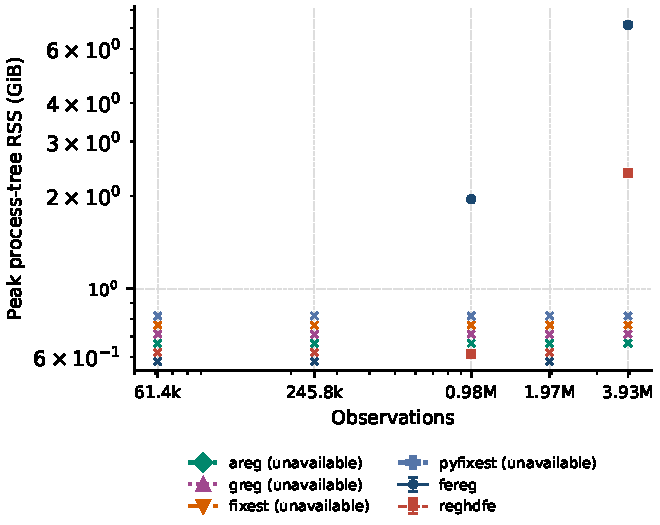
\includegraphics[width=\linewidth]{panels/absolute-ols-expanded-three_fe_sparse-maximum-peak_rss_gib.pdf}
\caption{RSS by observations}
\end{subfigure}\hfill
\begin{subfigure}[t]{0.485\linewidth}\centering
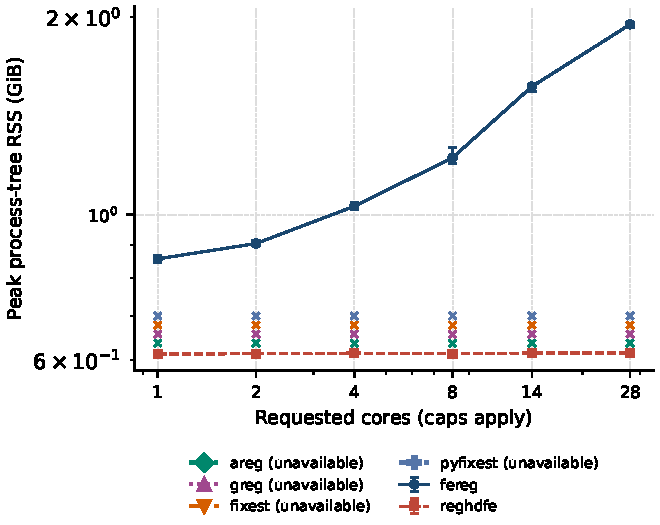
\includegraphics[width=\linewidth]{panels/absolute-ols-expanded-three_fe_sparse-cores-peak_rss_gib.pdf}
\caption{RSS by requested cores}
\end{subfigure}\par\medskip
\begin{minipage}{0.98\linewidth}\footnotesize Partial campaign. Points require all six valid warm repetitions; bars show IQR, not confidence intervals. Crosses mark missing or unvalidated points. Both axes are logarithmic. Every task reserves 28 cores; Stata-controlled computation is capped at four. OLS IID inference, ten controls. See runs.csv for exclusions.\end{minipage}
\end{figure}\clearpage

\begin{figure}[p]\centering
\caption{OLS Sparse three FE: expanded, fixed capacity}
\begin{subfigure}[t]{0.485\linewidth}\centering
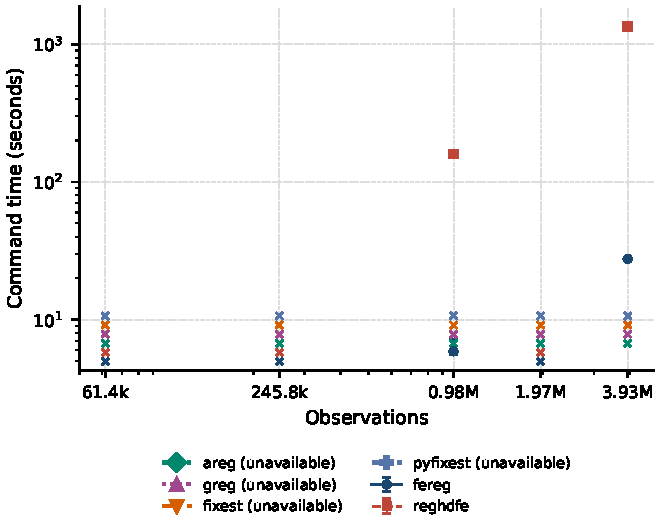
\includegraphics[width=\linewidth]{panels/absolute-ols-expanded-three_fe_sparse-fixed-seconds.pdf}
\caption{Time by observations}
\end{subfigure}\hfill
\begin{subfigure}[t]{0.485\linewidth}\centering
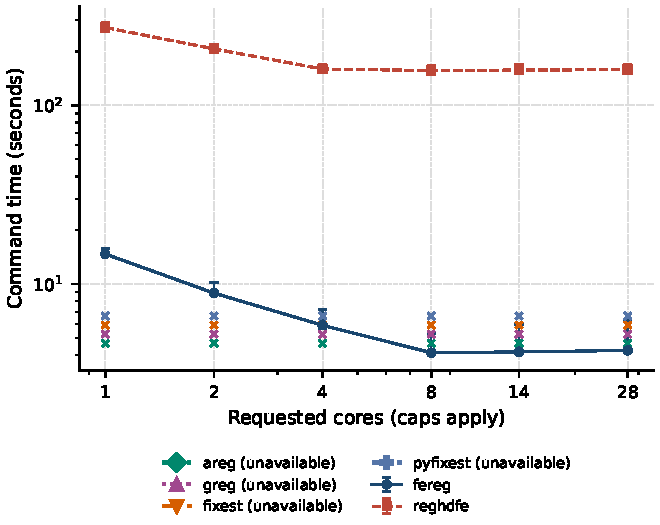
\includegraphics[width=\linewidth]{panels/absolute-ols-expanded-three_fe_sparse-cores-seconds.pdf}
\caption{Time by requested cores}
\end{subfigure}\par\medskip
\begin{subfigure}[t]{0.485\linewidth}\centering
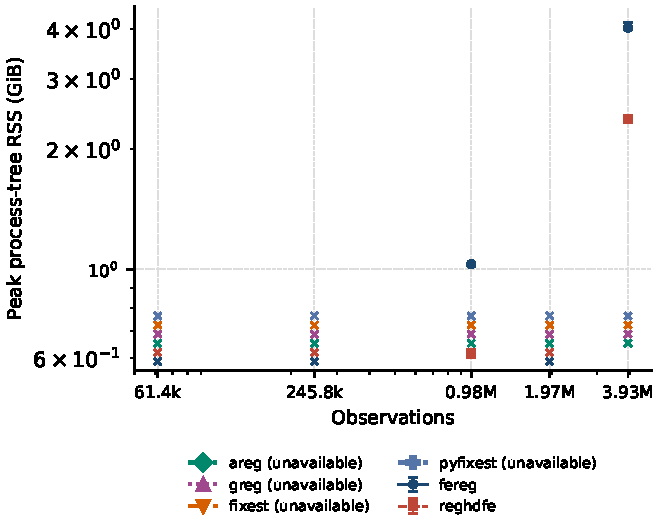
\includegraphics[width=\linewidth]{panels/absolute-ols-expanded-three_fe_sparse-fixed-peak_rss_gib.pdf}
\caption{RSS by observations}
\end{subfigure}\hfill
\begin{subfigure}[t]{0.485\linewidth}\centering
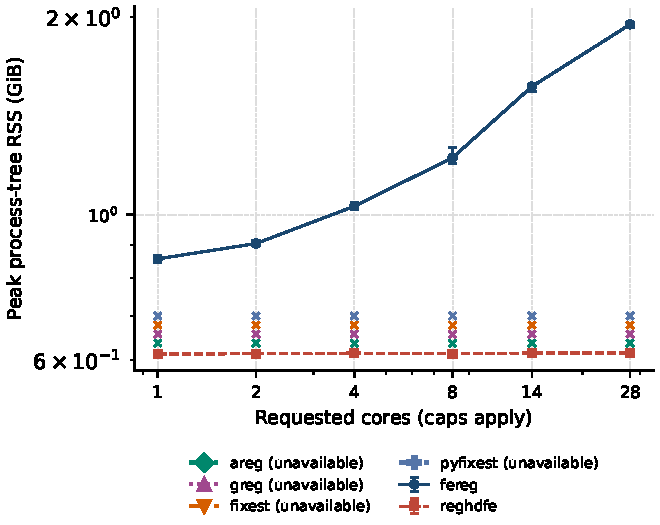
\includegraphics[width=\linewidth]{panels/absolute-ols-expanded-three_fe_sparse-cores-peak_rss_gib.pdf}
\caption{RSS by requested cores}
\end{subfigure}\par\medskip
\begin{minipage}{0.98\linewidth}\footnotesize Partial campaign. Points require all six valid warm repetitions; bars show IQR, not confidence intervals. Crosses mark missing or unvalidated points. Both axes are logarithmic. Every task reserves 28 cores; Stata-controlled computation is capped at four. OLS IID inference, ten controls. See runs.csv for exclusions.\end{minipage}
\end{figure}\clearpage

\begin{figure}[p]\centering
\caption{OLS Strong d=2: expanded, maximum capacity}
\begin{subfigure}[t]{0.485\linewidth}\centering
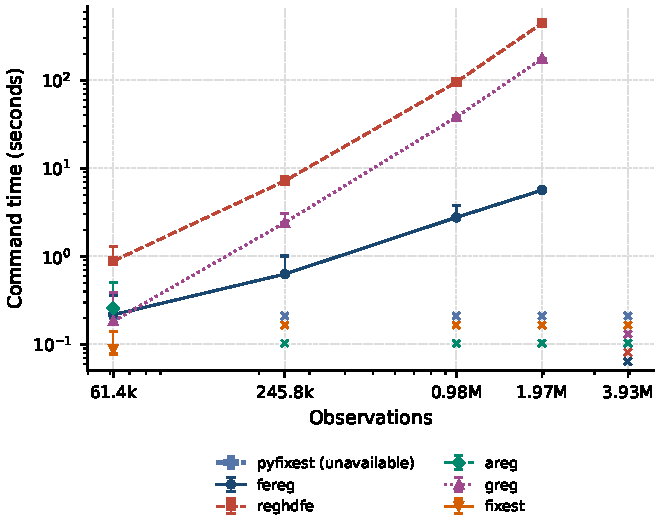
\includegraphics[width=\linewidth]{panels/absolute-ols-expanded-strong_d2-maximum-seconds.pdf}
\caption{Time by observations}
\end{subfigure}\hfill
\begin{subfigure}[t]{0.485\linewidth}\centering
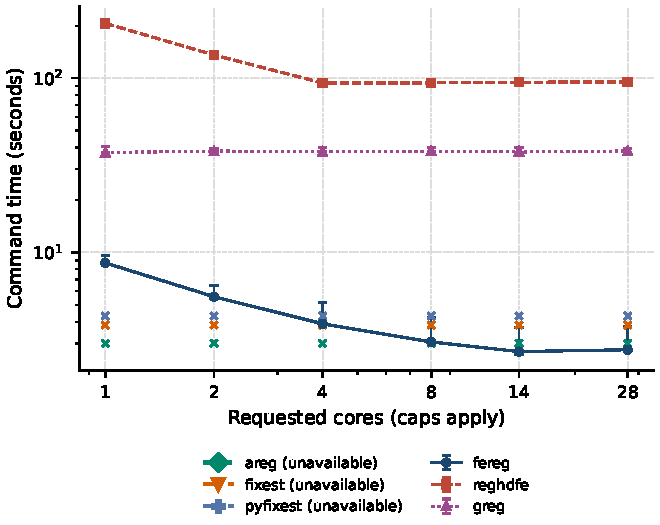
\includegraphics[width=\linewidth]{panels/absolute-ols-expanded-strong_d2-cores-seconds.pdf}
\caption{Time by requested cores}
\end{subfigure}\par\medskip
\begin{subfigure}[t]{0.485\linewidth}\centering
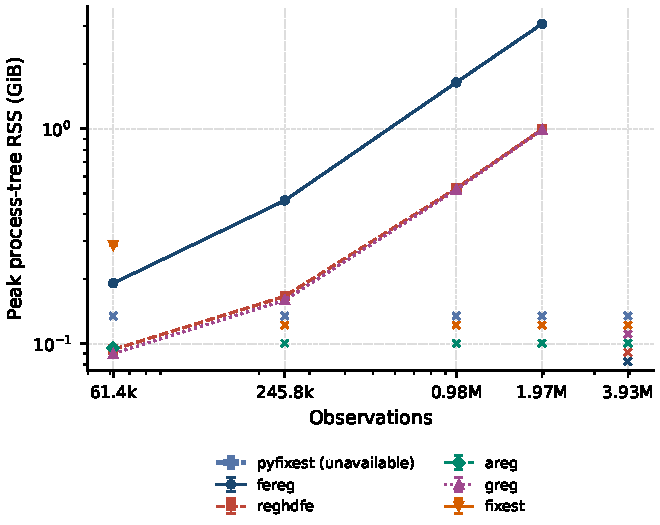
\includegraphics[width=\linewidth]{panels/absolute-ols-expanded-strong_d2-maximum-peak_rss_gib.pdf}
\caption{RSS by observations}
\end{subfigure}\hfill
\begin{subfigure}[t]{0.485\linewidth}\centering
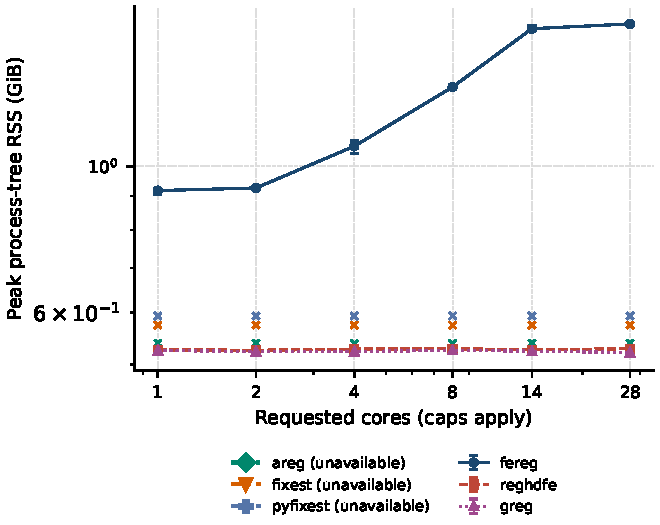
\includegraphics[width=\linewidth]{panels/absolute-ols-expanded-strong_d2-cores-peak_rss_gib.pdf}
\caption{RSS by requested cores}
\end{subfigure}\par\medskip
\begin{minipage}{0.98\linewidth}\footnotesize Partial campaign. Points require all six valid warm repetitions; bars show IQR, not confidence intervals. Crosses mark missing or unvalidated points. Both axes are logarithmic. Every task reserves 28 cores; Stata-controlled computation is capped at four. OLS IID inference, ten controls. See runs.csv for exclusions.\end{minipage}
\end{figure}\clearpage

\begin{figure}[p]\centering
\caption{OLS Strong d=2: expanded, fixed capacity}
\begin{subfigure}[t]{0.485\linewidth}\centering
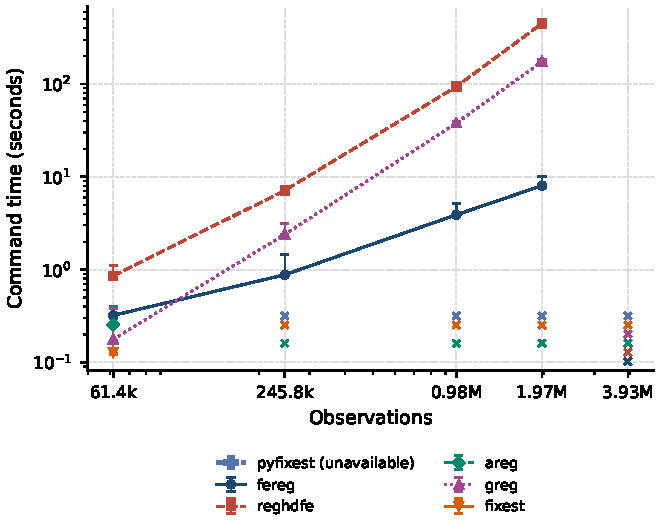
\includegraphics[width=\linewidth]{panels/absolute-ols-expanded-strong_d2-fixed-seconds.pdf}
\caption{Time by observations}
\end{subfigure}\hfill
\begin{subfigure}[t]{0.485\linewidth}\centering
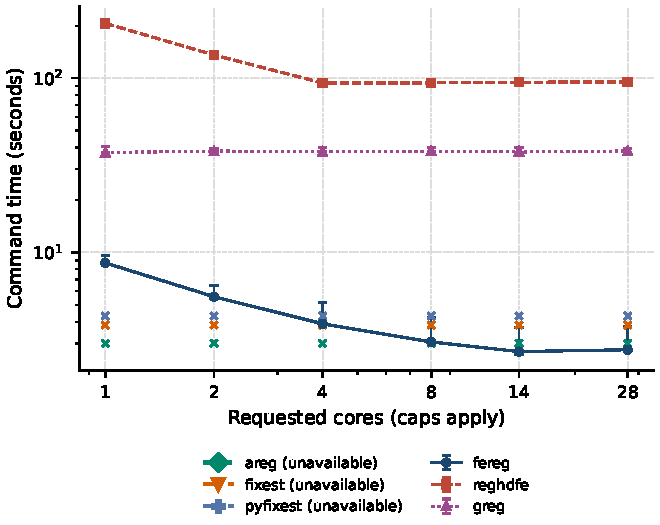
\includegraphics[width=\linewidth]{panels/absolute-ols-expanded-strong_d2-cores-seconds.pdf}
\caption{Time by requested cores}
\end{subfigure}\par\medskip
\begin{subfigure}[t]{0.485\linewidth}\centering
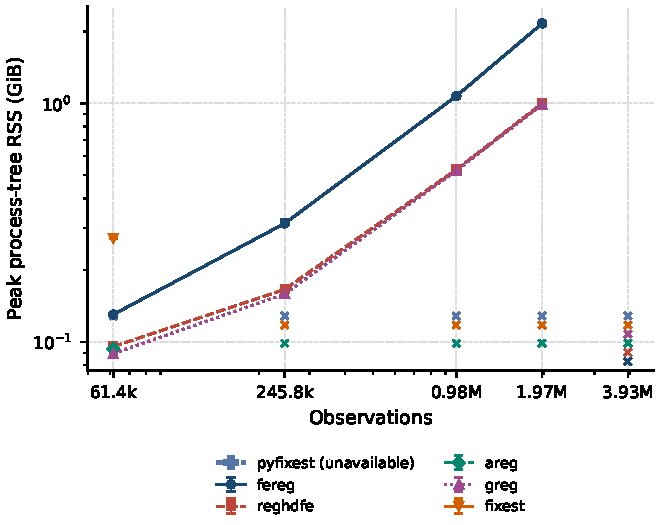
\includegraphics[width=\linewidth]{panels/absolute-ols-expanded-strong_d2-fixed-peak_rss_gib.pdf}
\caption{RSS by observations}
\end{subfigure}\hfill
\begin{subfigure}[t]{0.485\linewidth}\centering
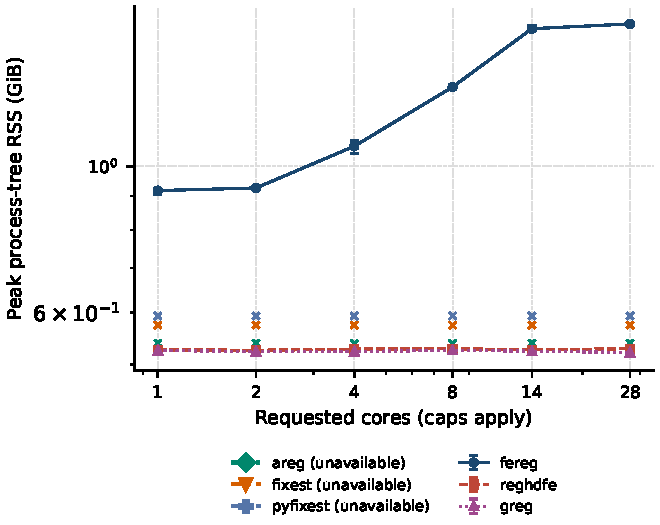
\includegraphics[width=\linewidth]{panels/absolute-ols-expanded-strong_d2-cores-peak_rss_gib.pdf}
\caption{RSS by requested cores}
\end{subfigure}\par\medskip
\begin{minipage}{0.98\linewidth}\footnotesize Partial campaign. Points require all six valid warm repetitions; bars show IQR, not confidence intervals. Crosses mark missing or unvalidated points. Both axes are logarithmic. Every task reserves 28 cores; Stata-controlled computation is capped at four. OLS IID inference, ten controls. See runs.csv for exclusions.\end{minipage}
\end{figure}\clearpage

\begin{figure}[p]\centering
\caption{OLS Strong d=3: expanded, maximum capacity}
\begin{subfigure}[t]{0.485\linewidth}\centering
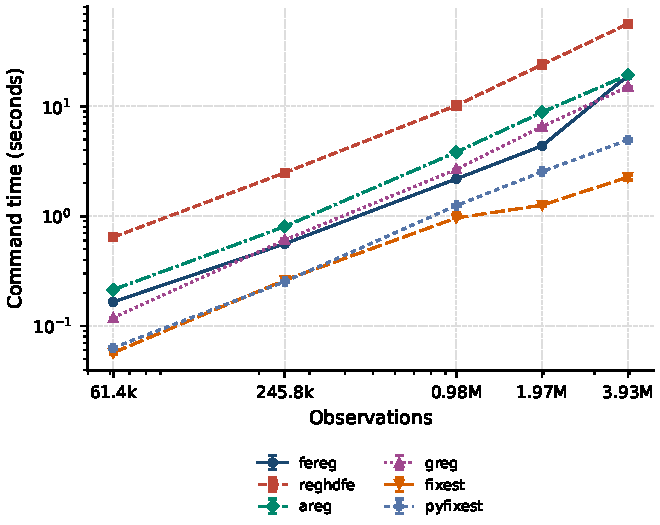
\includegraphics[width=\linewidth]{panels/absolute-ols-expanded-strong_d3-maximum-seconds.pdf}
\caption{Time by observations}
\end{subfigure}\hfill
\begin{subfigure}[t]{0.485\linewidth}\centering
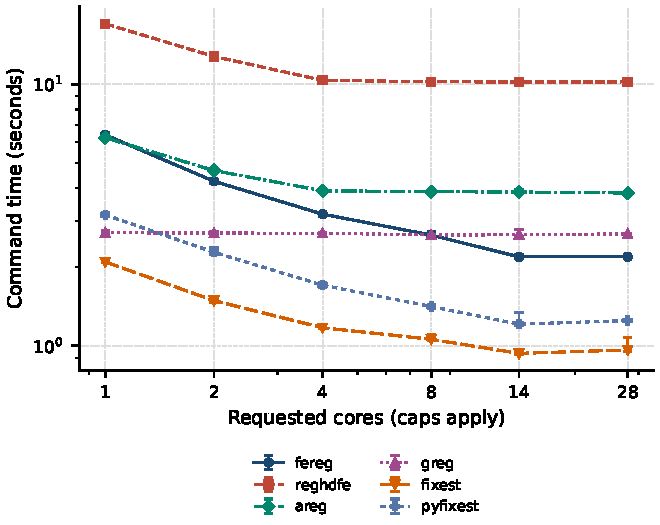
\includegraphics[width=\linewidth]{panels/absolute-ols-expanded-strong_d3-cores-seconds.pdf}
\caption{Time by requested cores}
\end{subfigure}\par\medskip
\begin{subfigure}[t]{0.485\linewidth}\centering
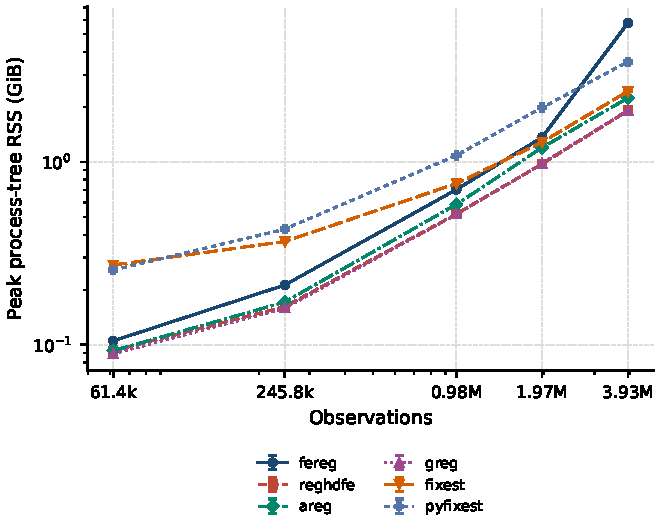
\includegraphics[width=\linewidth]{panels/absolute-ols-expanded-strong_d3-maximum-peak_rss_gib.pdf}
\caption{RSS by observations}
\end{subfigure}\hfill
\begin{subfigure}[t]{0.485\linewidth}\centering
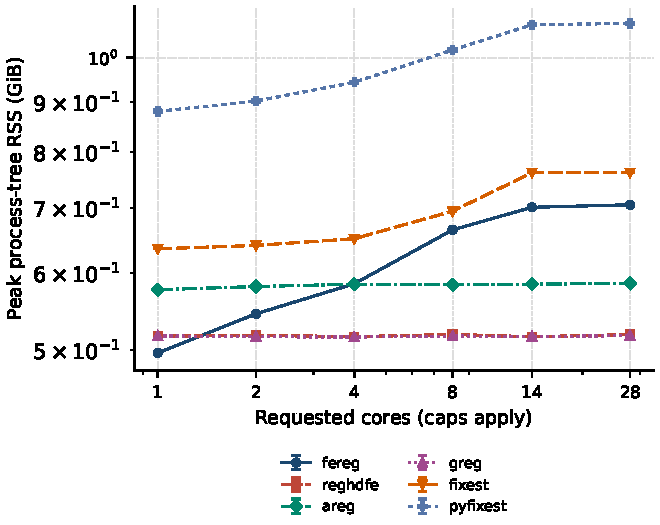
\includegraphics[width=\linewidth]{panels/absolute-ols-expanded-strong_d3-cores-peak_rss_gib.pdf}
\caption{RSS by requested cores}
\end{subfigure}\par\medskip
\begin{minipage}{0.98\linewidth}\footnotesize Partial campaign. Points require all six valid warm repetitions; bars show IQR, not confidence intervals. Crosses mark missing or unvalidated points. Both axes are logarithmic. Every task reserves 28 cores; Stata-controlled computation is capped at four. OLS IID inference, ten controls. See runs.csv for exclusions.\end{minipage}
\end{figure}\clearpage

\begin{figure}[p]\centering
\caption{OLS Strong d=3: expanded, fixed capacity}
\begin{subfigure}[t]{0.485\linewidth}\centering
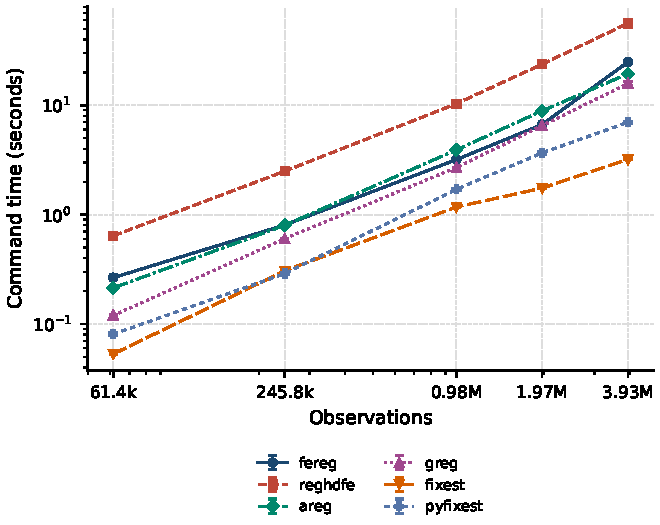
\includegraphics[width=\linewidth]{panels/absolute-ols-expanded-strong_d3-fixed-seconds.pdf}
\caption{Time by observations}
\end{subfigure}\hfill
\begin{subfigure}[t]{0.485\linewidth}\centering
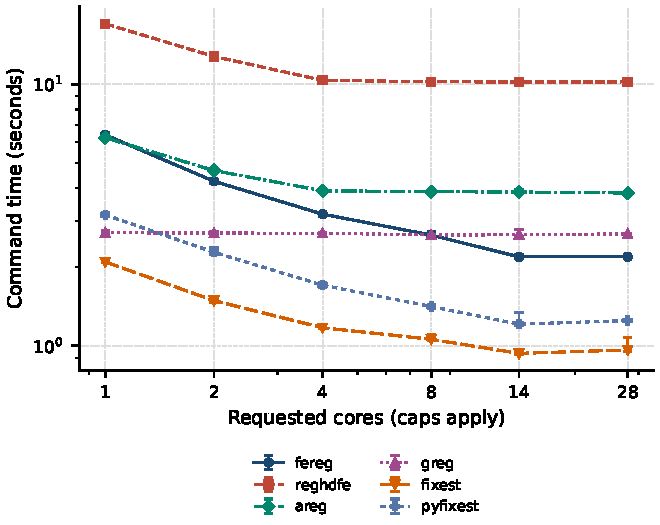
\includegraphics[width=\linewidth]{panels/absolute-ols-expanded-strong_d3-cores-seconds.pdf}
\caption{Time by requested cores}
\end{subfigure}\par\medskip
\begin{subfigure}[t]{0.485\linewidth}\centering
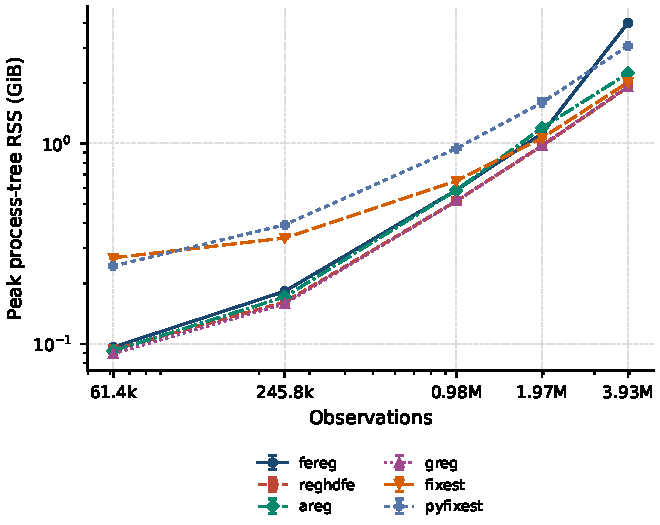
\includegraphics[width=\linewidth]{panels/absolute-ols-expanded-strong_d3-fixed-peak_rss_gib.pdf}
\caption{RSS by observations}
\end{subfigure}\hfill
\begin{subfigure}[t]{0.485\linewidth}\centering
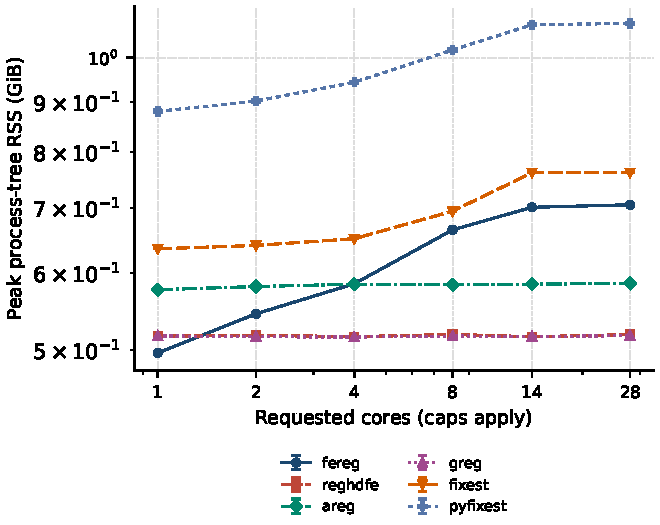
\includegraphics[width=\linewidth]{panels/absolute-ols-expanded-strong_d3-cores-peak_rss_gib.pdf}
\caption{RSS by requested cores}
\end{subfigure}\par\medskip
\begin{minipage}{0.98\linewidth}\footnotesize Partial campaign. Points require all six valid warm repetitions; bars show IQR, not confidence intervals. Crosses mark missing or unvalidated points. Both axes are logarithmic. Every task reserves 28 cores; Stata-controlled computation is capped at four. OLS IID inference, ten controls. See runs.csv for exclusions.\end{minipage}
\end{figure}\clearpage

\begin{figure}[p]\centering
\caption{OLS Strong d=6: expanded, maximum capacity}
\begin{subfigure}[t]{0.485\linewidth}\centering
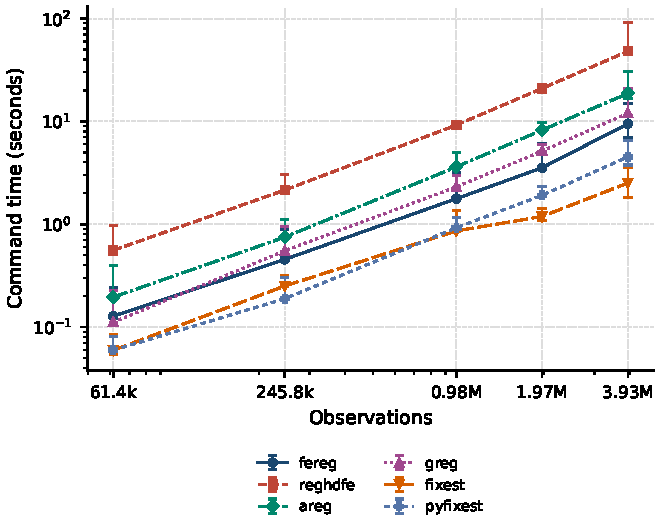
\includegraphics[width=\linewidth]{panels/absolute-ols-expanded-strong_d6-maximum-seconds.pdf}
\caption{Time by observations}
\end{subfigure}\hfill
\begin{subfigure}[t]{0.485\linewidth}\centering
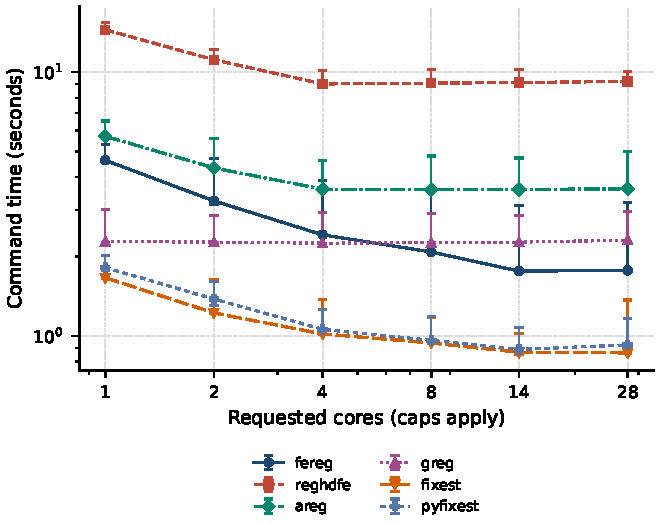
\includegraphics[width=\linewidth]{panels/absolute-ols-expanded-strong_d6-cores-seconds.pdf}
\caption{Time by requested cores}
\end{subfigure}\par\medskip
\begin{subfigure}[t]{0.485\linewidth}\centering
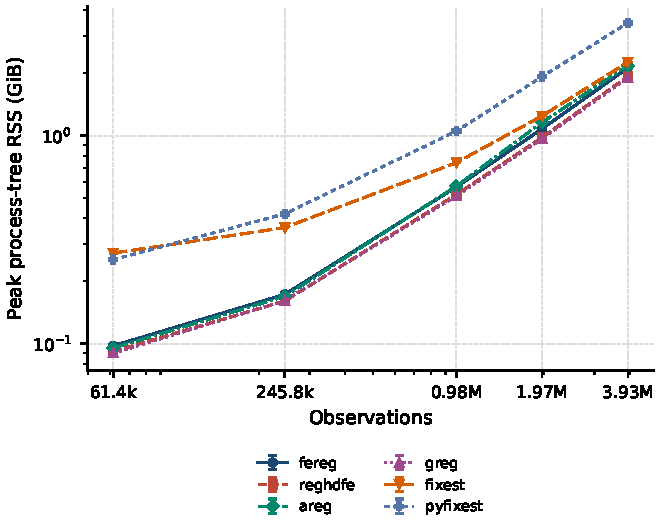
\includegraphics[width=\linewidth]{panels/absolute-ols-expanded-strong_d6-maximum-peak_rss_gib.pdf}
\caption{RSS by observations}
\end{subfigure}\hfill
\begin{subfigure}[t]{0.485\linewidth}\centering
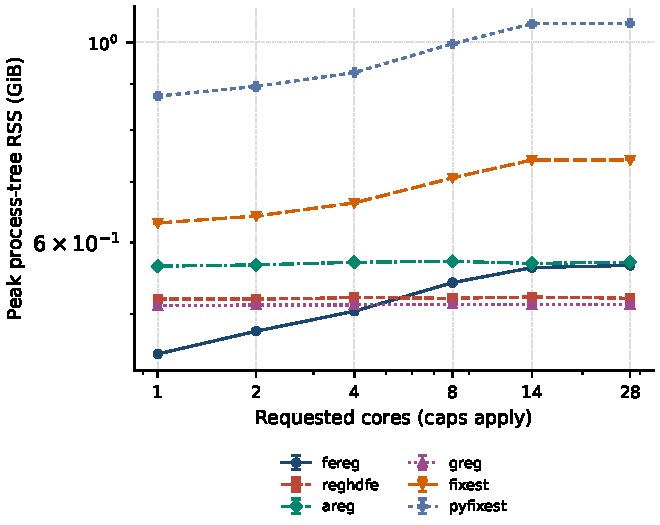
\includegraphics[width=\linewidth]{panels/absolute-ols-expanded-strong_d6-cores-peak_rss_gib.pdf}
\caption{RSS by requested cores}
\end{subfigure}\par\medskip
\begin{minipage}{0.98\linewidth}\footnotesize Partial campaign. Points require all six valid warm repetitions; bars show IQR, not confidence intervals. Crosses mark missing or unvalidated points. Both axes are logarithmic. Every task reserves 28 cores; Stata-controlled computation is capped at four. OLS IID inference, ten controls. See runs.csv for exclusions.\end{minipage}
\end{figure}\clearpage

\begin{figure}[p]\centering
\caption{OLS Strong d=6: expanded, fixed capacity}
\begin{subfigure}[t]{0.485\linewidth}\centering
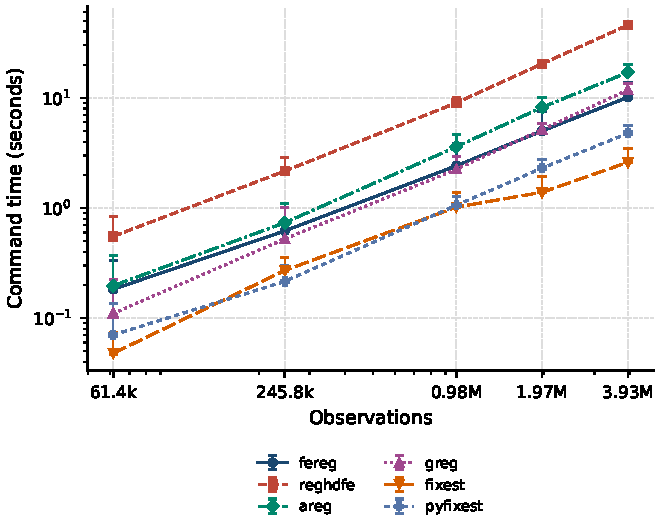
\includegraphics[width=\linewidth]{panels/absolute-ols-expanded-strong_d6-fixed-seconds.pdf}
\caption{Time by observations}
\end{subfigure}\hfill
\begin{subfigure}[t]{0.485\linewidth}\centering
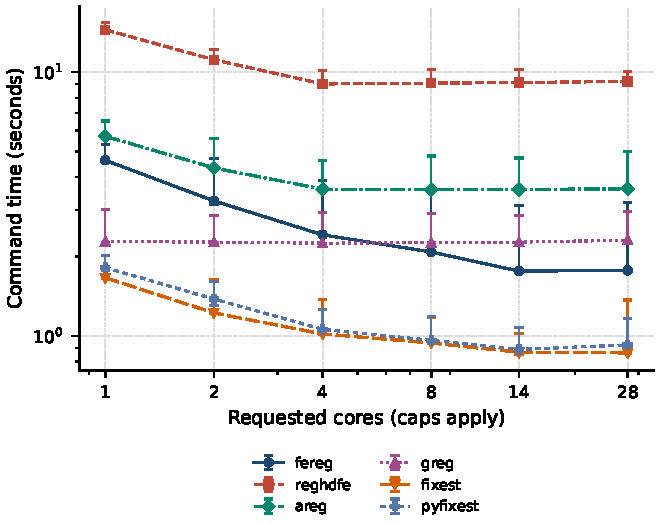
\includegraphics[width=\linewidth]{panels/absolute-ols-expanded-strong_d6-cores-seconds.pdf}
\caption{Time by requested cores}
\end{subfigure}\par\medskip
\begin{subfigure}[t]{0.485\linewidth}\centering
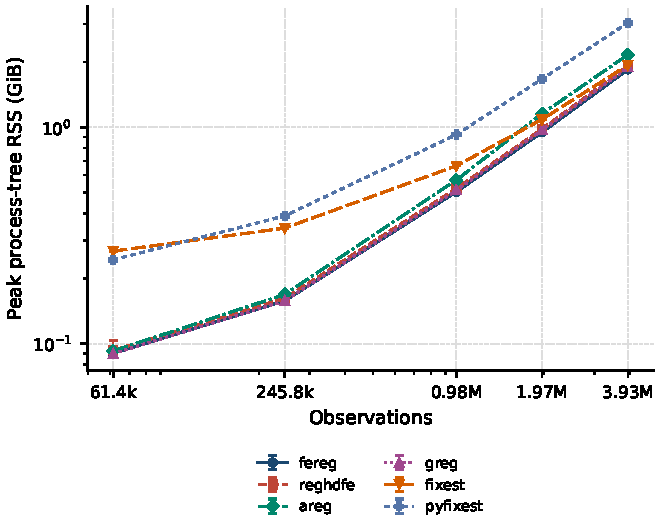
\includegraphics[width=\linewidth]{panels/absolute-ols-expanded-strong_d6-fixed-peak_rss_gib.pdf}
\caption{RSS by observations}
\end{subfigure}\hfill
\begin{subfigure}[t]{0.485\linewidth}\centering
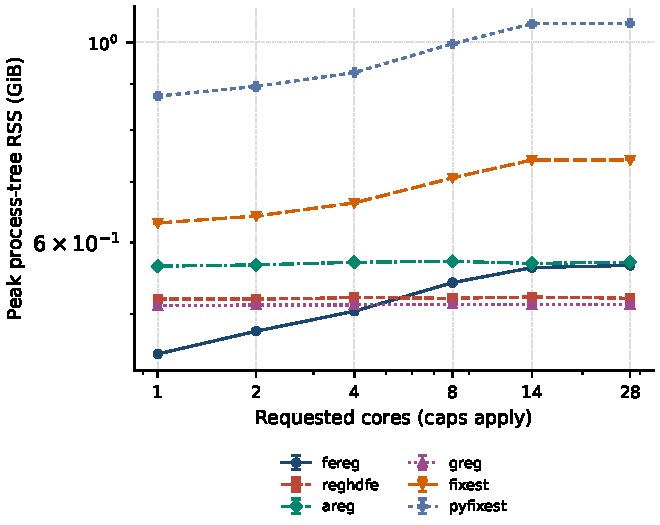
\includegraphics[width=\linewidth]{panels/absolute-ols-expanded-strong_d6-cores-peak_rss_gib.pdf}
\caption{RSS by requested cores}
\end{subfigure}\par\medskip
\begin{minipage}{0.98\linewidth}\footnotesize Partial campaign. Points require all six valid warm repetitions; bars show IQR, not confidence intervals. Crosses mark missing or unvalidated points. Both axes are logarithmic. Every task reserves 28 cores; Stata-controlled computation is capped at four. OLS IID inference, ten controls. See runs.csv for exclusions.\end{minipage}
\end{figure}\clearpage

\begin{figure}[p]\centering
\caption{fereg/reghdfe: panels, maximum capacity}
\begin{subfigure}[t]{0.485\linewidth}\centering
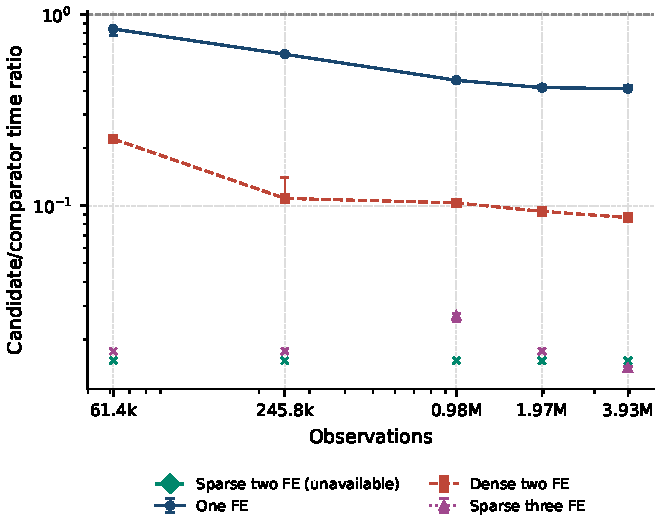
\includegraphics[width=\linewidth]{panels/ratio-ols-panels-reghdfe-maximum-seconds.pdf}
\caption{Time ratios by observations}
\end{subfigure}\hfill
\begin{subfigure}[t]{0.485\linewidth}\centering
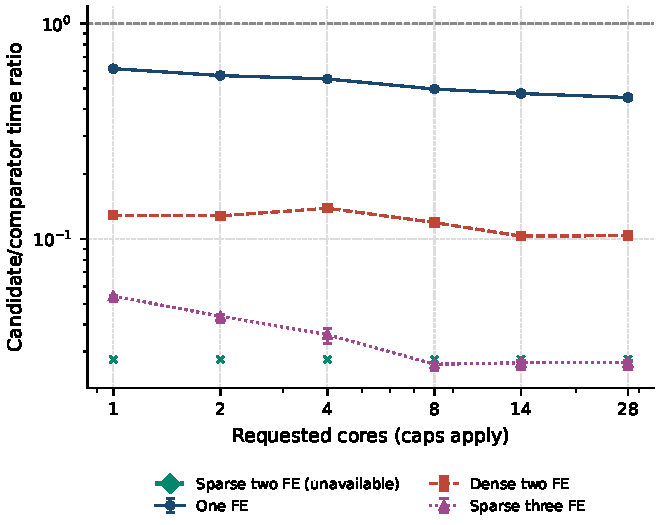
\includegraphics[width=\linewidth]{panels/ratio-ols-panels-reghdfe-cores-seconds.pdf}
\caption{Time ratios by requested cores}
\end{subfigure}\par\medskip
\begin{subfigure}[t]{0.485\linewidth}\centering
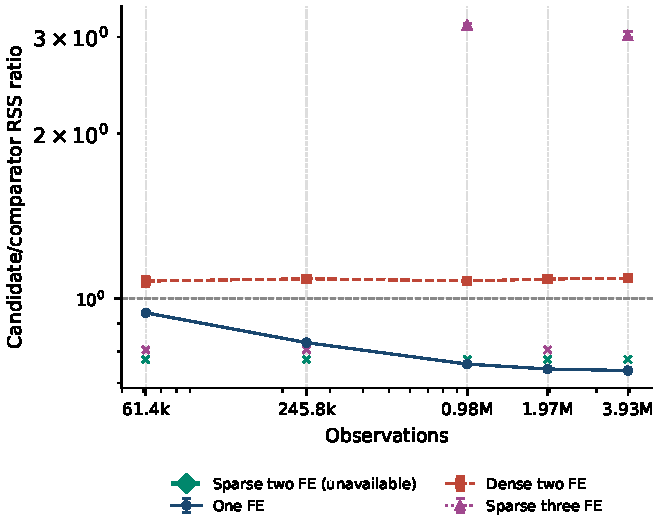
\includegraphics[width=\linewidth]{panels/ratio-ols-panels-reghdfe-maximum-peak_rss_gib.pdf}
\caption{RSS ratios by observations}
\end{subfigure}\hfill
\begin{subfigure}[t]{0.485\linewidth}\centering
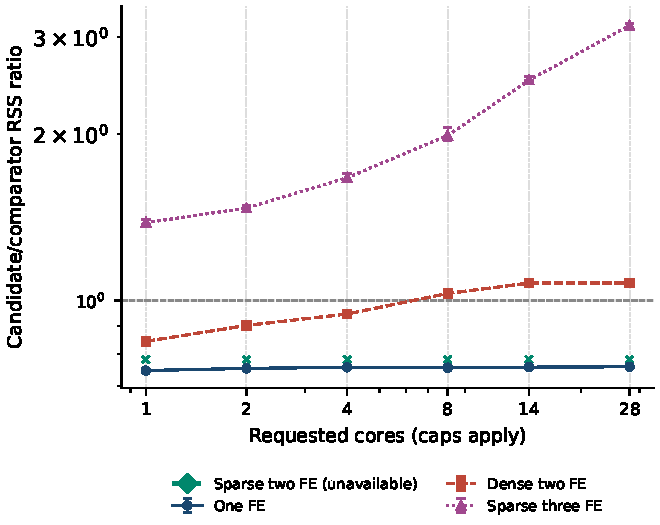
\includegraphics[width=\linewidth]{panels/ratio-ols-panels-reghdfe-cores-peak_rss_gib.pdf}
\caption{RSS ratios by requested cores}
\end{subfigure}\par\medskip
\begin{minipage}{0.98\linewidth}\footnotesize Partial campaign. Points require all six valid warm repetitions; bars show IQR, not confidence intervals. Crosses mark missing or unvalidated points. Both axes are logarithmic. Every task reserves 28 cores; Stata-controlled computation is capped at four. OLS IID inference, ten controls. See runs.csv for exclusions. Ratios are computed within seed/node pairs. Values below one favor fereg.\end{minipage}
\end{figure}\clearpage

\begin{figure}[p]\centering
\caption{fereg/reghdfe: panels, fixed capacity}
\begin{subfigure}[t]{0.485\linewidth}\centering
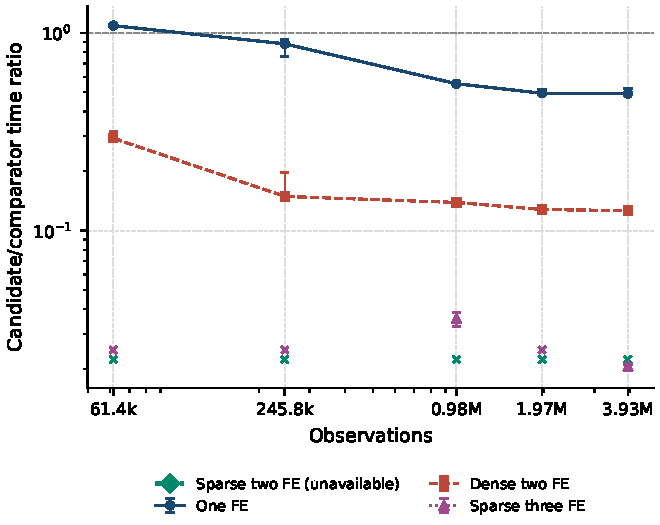
\includegraphics[width=\linewidth]{panels/ratio-ols-panels-reghdfe-fixed-seconds.pdf}
\caption{Time ratios by observations}
\end{subfigure}\hfill
\begin{subfigure}[t]{0.485\linewidth}\centering
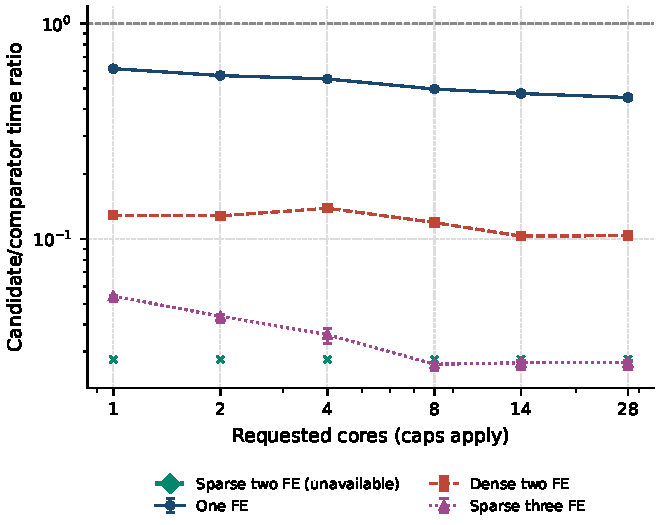
\includegraphics[width=\linewidth]{panels/ratio-ols-panels-reghdfe-cores-seconds.pdf}
\caption{Time ratios by requested cores}
\end{subfigure}\par\medskip
\begin{subfigure}[t]{0.485\linewidth}\centering
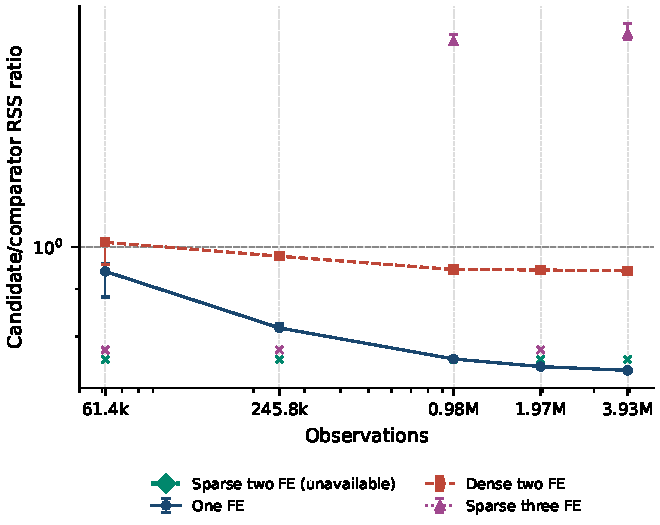
\includegraphics[width=\linewidth]{panels/ratio-ols-panels-reghdfe-fixed-peak_rss_gib.pdf}
\caption{RSS ratios by observations}
\end{subfigure}\hfill
\begin{subfigure}[t]{0.485\linewidth}\centering
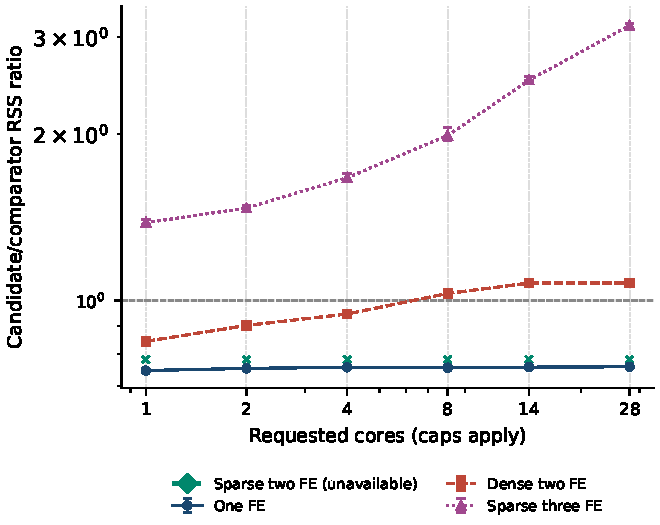
\includegraphics[width=\linewidth]{panels/ratio-ols-panels-reghdfe-cores-peak_rss_gib.pdf}
\caption{RSS ratios by requested cores}
\end{subfigure}\par\medskip
\begin{minipage}{0.98\linewidth}\footnotesize Partial campaign. Points require all six valid warm repetitions; bars show IQR, not confidence intervals. Crosses mark missing or unvalidated points. Both axes are logarithmic. Every task reserves 28 cores; Stata-controlled computation is capped at four. OLS IID inference, ten controls. See runs.csv for exclusions. Ratios are computed within seed/node pairs. Values below one favor fereg.\end{minipage}
\end{figure}\clearpage

\begin{figure}[p]\centering
\caption{fereg/areg: panels, maximum capacity}
\begin{subfigure}[t]{0.485\linewidth}\centering
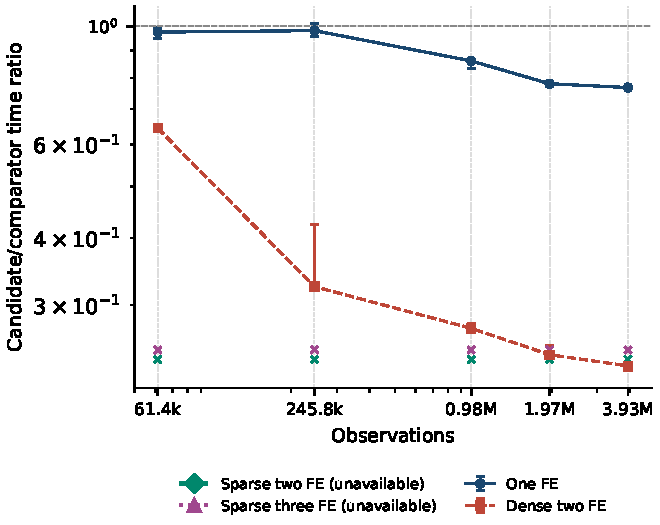
\includegraphics[width=\linewidth]{panels/ratio-ols-panels-areg-maximum-seconds.pdf}
\caption{Time ratios by observations}
\end{subfigure}\hfill
\begin{subfigure}[t]{0.485\linewidth}\centering
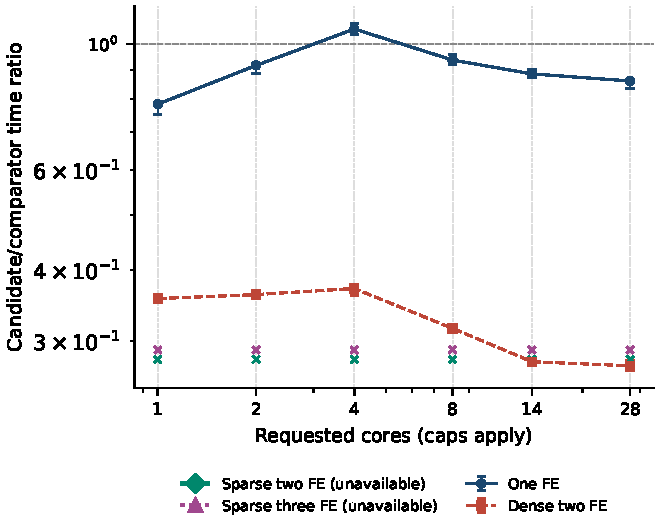
\includegraphics[width=\linewidth]{panels/ratio-ols-panels-areg-cores-seconds.pdf}
\caption{Time ratios by requested cores}
\end{subfigure}\par\medskip
\begin{subfigure}[t]{0.485\linewidth}\centering
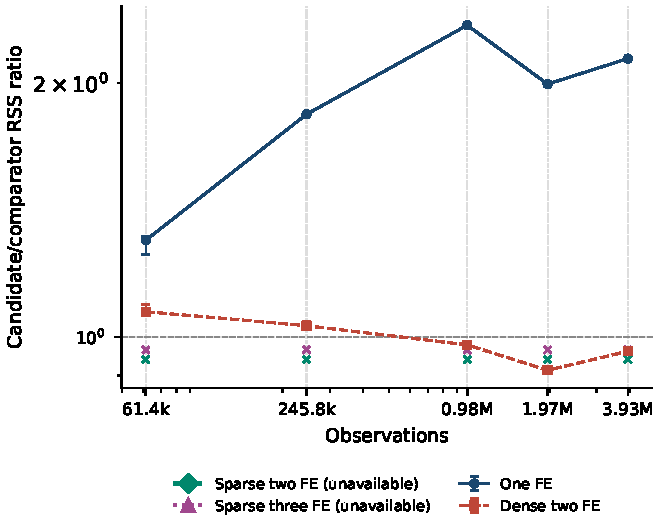
\includegraphics[width=\linewidth]{panels/ratio-ols-panels-areg-maximum-peak_rss_gib.pdf}
\caption{RSS ratios by observations}
\end{subfigure}\hfill
\begin{subfigure}[t]{0.485\linewidth}\centering
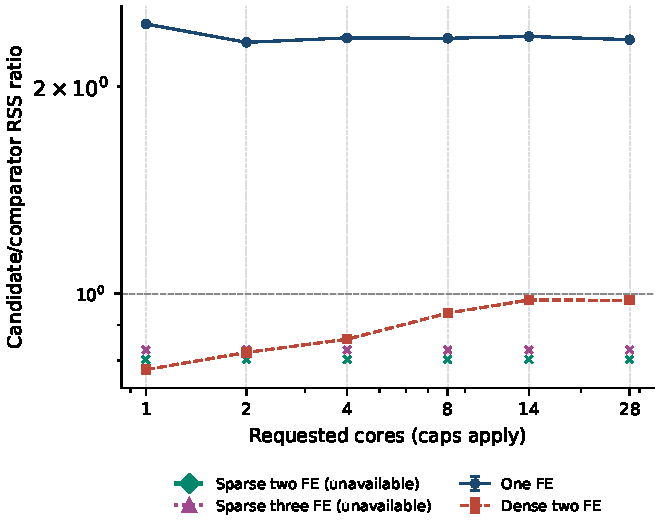
\includegraphics[width=\linewidth]{panels/ratio-ols-panels-areg-cores-peak_rss_gib.pdf}
\caption{RSS ratios by requested cores}
\end{subfigure}\par\medskip
\begin{minipage}{0.98\linewidth}\footnotesize Partial campaign. Points require all six valid warm repetitions; bars show IQR, not confidence intervals. Crosses mark missing or unvalidated points. Both axes are logarithmic. Every task reserves 28 cores; Stata-controlled computation is capped at four. OLS IID inference, ten controls. See runs.csv for exclusions. Ratios are computed within seed/node pairs. Values below one favor fereg.\end{minipage}
\end{figure}\clearpage

\begin{figure}[p]\centering
\caption{fereg/areg: panels, fixed capacity}
\begin{subfigure}[t]{0.485\linewidth}\centering
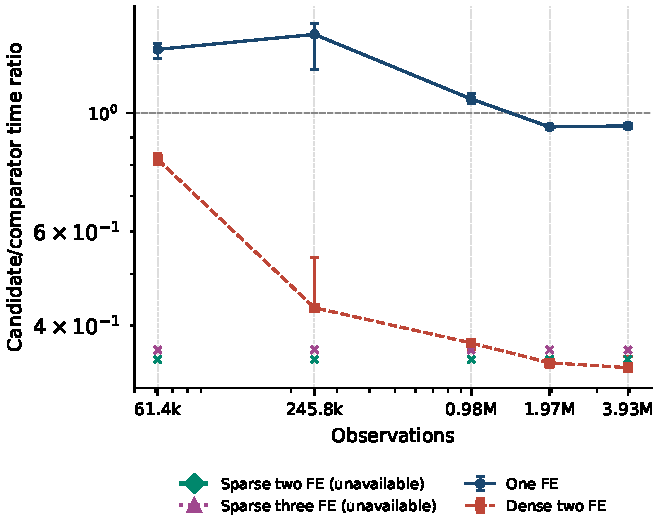
\includegraphics[width=\linewidth]{panels/ratio-ols-panels-areg-fixed-seconds.pdf}
\caption{Time ratios by observations}
\end{subfigure}\hfill
\begin{subfigure}[t]{0.485\linewidth}\centering
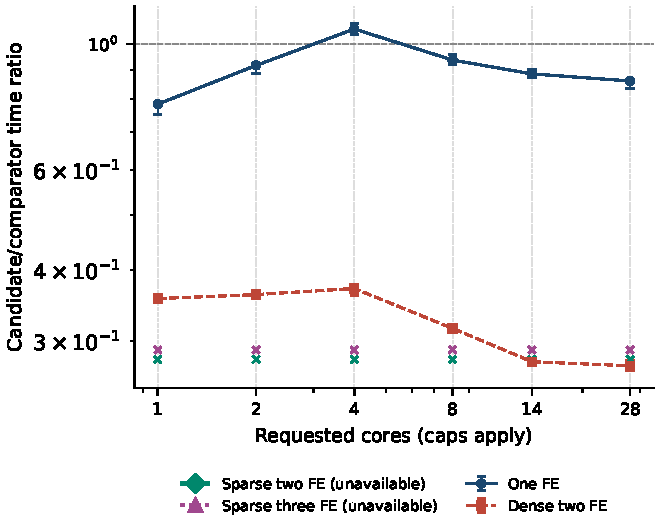
\includegraphics[width=\linewidth]{panels/ratio-ols-panels-areg-cores-seconds.pdf}
\caption{Time ratios by requested cores}
\end{subfigure}\par\medskip
\begin{subfigure}[t]{0.485\linewidth}\centering
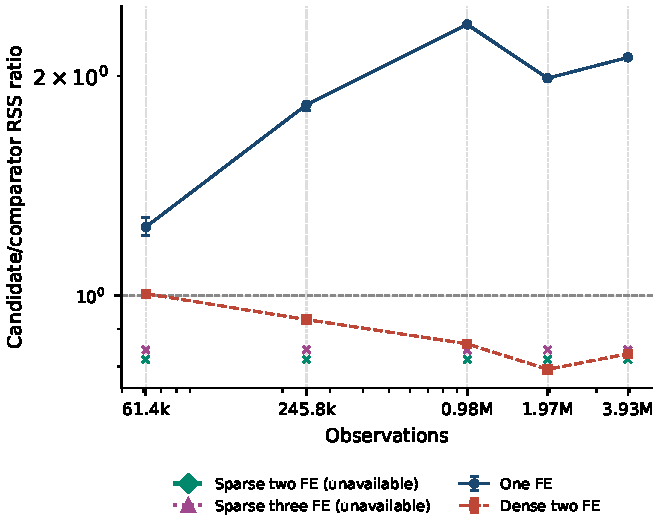
\includegraphics[width=\linewidth]{panels/ratio-ols-panels-areg-fixed-peak_rss_gib.pdf}
\caption{RSS ratios by observations}
\end{subfigure}\hfill
\begin{subfigure}[t]{0.485\linewidth}\centering
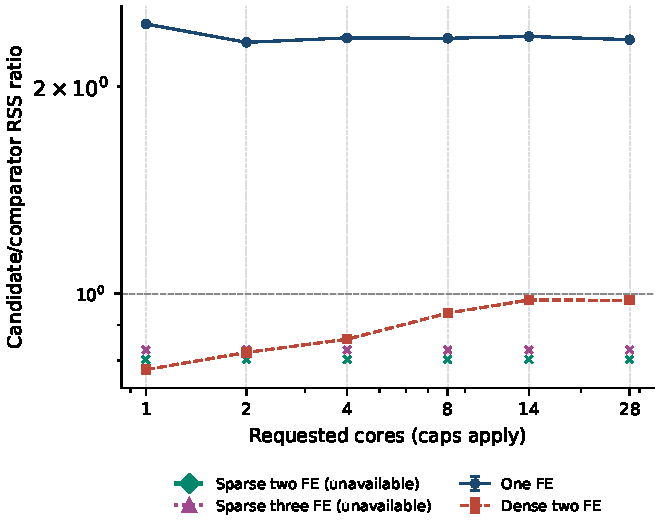
\includegraphics[width=\linewidth]{panels/ratio-ols-panels-areg-cores-peak_rss_gib.pdf}
\caption{RSS ratios by requested cores}
\end{subfigure}\par\medskip
\begin{minipage}{0.98\linewidth}\footnotesize Partial campaign. Points require all six valid warm repetitions; bars show IQR, not confidence intervals. Crosses mark missing or unvalidated points. Both axes are logarithmic. Every task reserves 28 cores; Stata-controlled computation is capped at four. OLS IID inference, ten controls. See runs.csv for exclusions. Ratios are computed within seed/node pairs. Values below one favor fereg.\end{minipage}
\end{figure}\clearpage

\begin{figure}[p]\centering
\caption{fereg/greg: panels, maximum capacity}
\begin{subfigure}[t]{0.485\linewidth}\centering
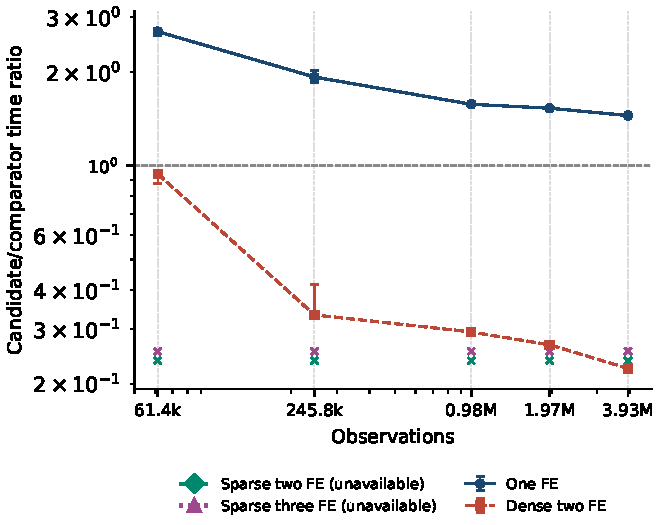
\includegraphics[width=\linewidth]{panels/ratio-ols-panels-greg-maximum-seconds.pdf}
\caption{Time ratios by observations}
\end{subfigure}\hfill
\begin{subfigure}[t]{0.485\linewidth}\centering
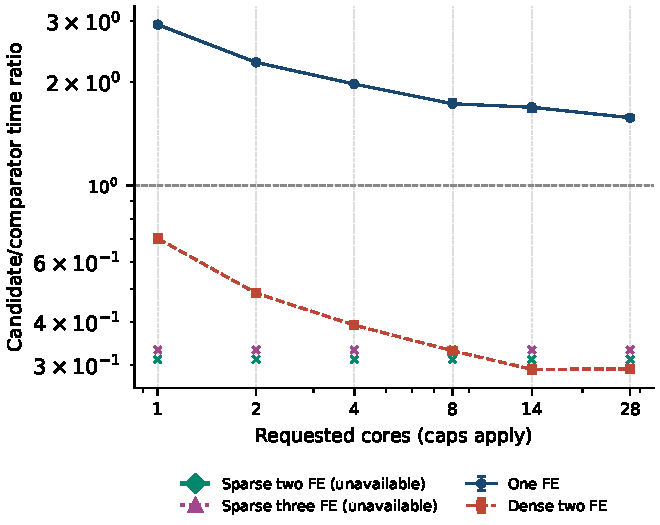
\includegraphics[width=\linewidth]{panels/ratio-ols-panels-greg-cores-seconds.pdf}
\caption{Time ratios by requested cores}
\end{subfigure}\par\medskip
\begin{subfigure}[t]{0.485\linewidth}\centering
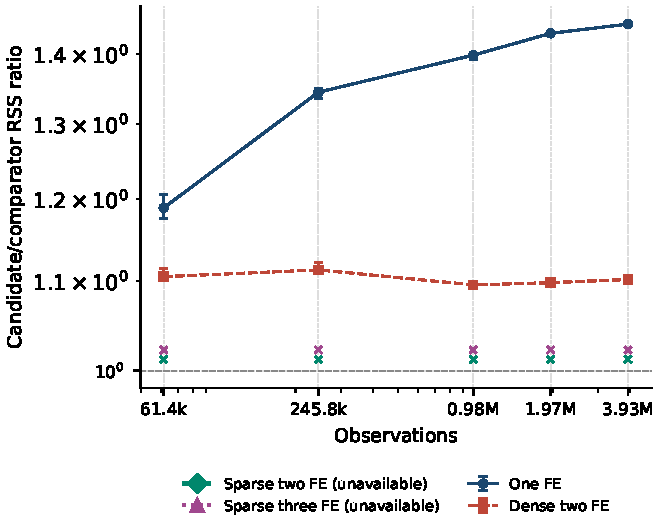
\includegraphics[width=\linewidth]{panels/ratio-ols-panels-greg-maximum-peak_rss_gib.pdf}
\caption{RSS ratios by observations}
\end{subfigure}\hfill
\begin{subfigure}[t]{0.485\linewidth}\centering
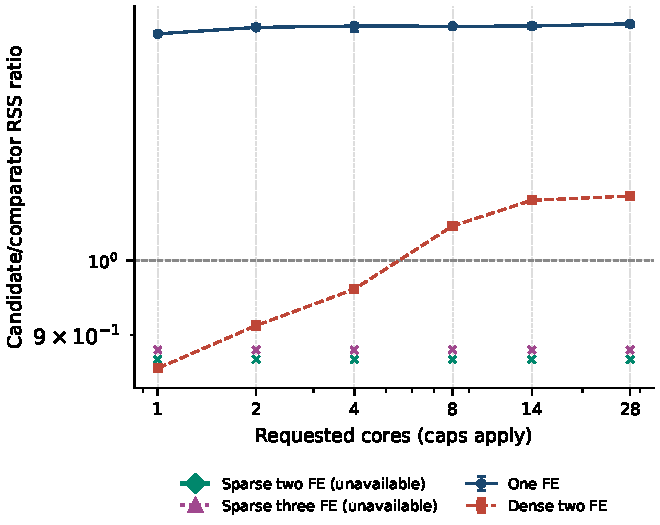
\includegraphics[width=\linewidth]{panels/ratio-ols-panels-greg-cores-peak_rss_gib.pdf}
\caption{RSS ratios by requested cores}
\end{subfigure}\par\medskip
\begin{minipage}{0.98\linewidth}\footnotesize Partial campaign. Points require all six valid warm repetitions; bars show IQR, not confidence intervals. Crosses mark missing or unvalidated points. Both axes are logarithmic. Every task reserves 28 cores; Stata-controlled computation is capped at four. OLS IID inference, ten controls. See runs.csv for exclusions. Ratios are computed within seed/node pairs. Values below one favor fereg.\end{minipage}
\end{figure}\clearpage

\begin{figure}[p]\centering
\caption{fereg/greg: panels, fixed capacity}
\begin{subfigure}[t]{0.485\linewidth}\centering
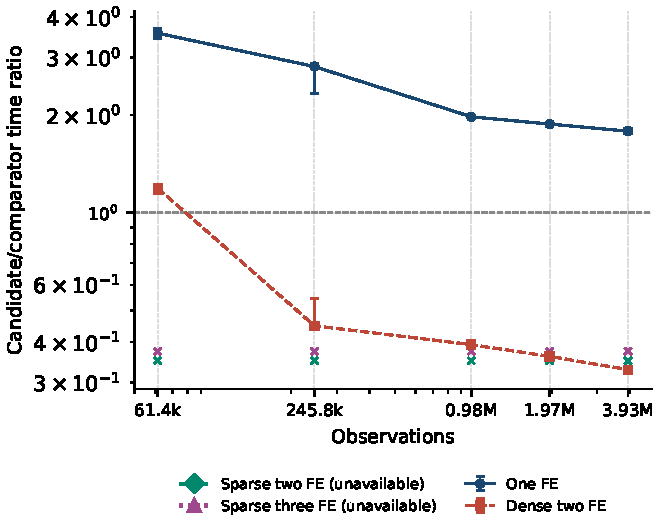
\includegraphics[width=\linewidth]{panels/ratio-ols-panels-greg-fixed-seconds.pdf}
\caption{Time ratios by observations}
\end{subfigure}\hfill
\begin{subfigure}[t]{0.485\linewidth}\centering
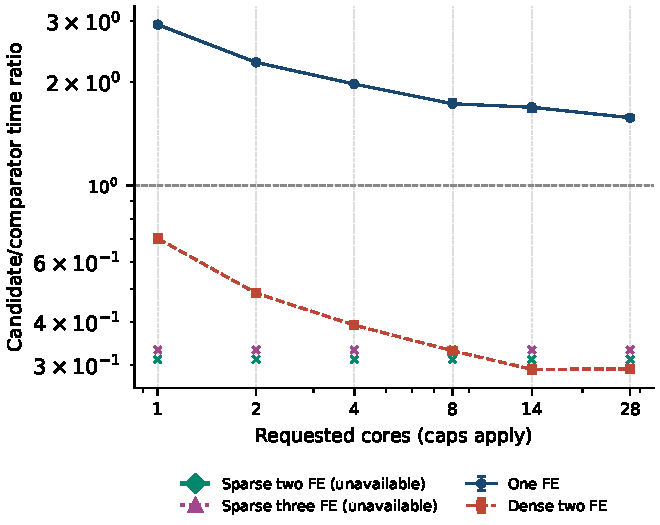
\includegraphics[width=\linewidth]{panels/ratio-ols-panels-greg-cores-seconds.pdf}
\caption{Time ratios by requested cores}
\end{subfigure}\par\medskip
\begin{subfigure}[t]{0.485\linewidth}\centering
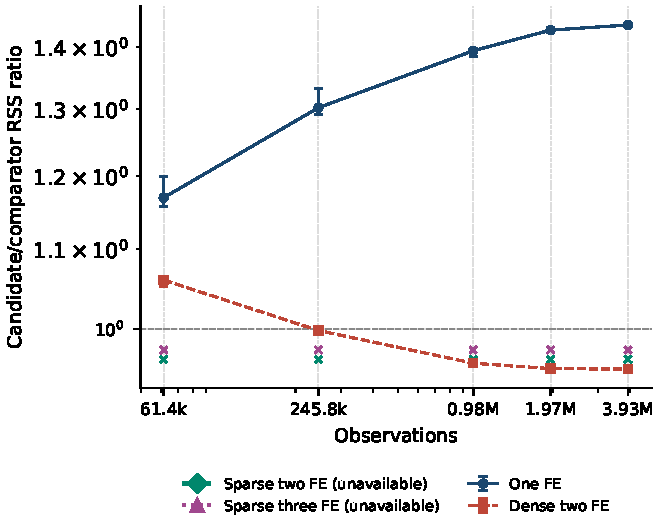
\includegraphics[width=\linewidth]{panels/ratio-ols-panels-greg-fixed-peak_rss_gib.pdf}
\caption{RSS ratios by observations}
\end{subfigure}\hfill
\begin{subfigure}[t]{0.485\linewidth}\centering
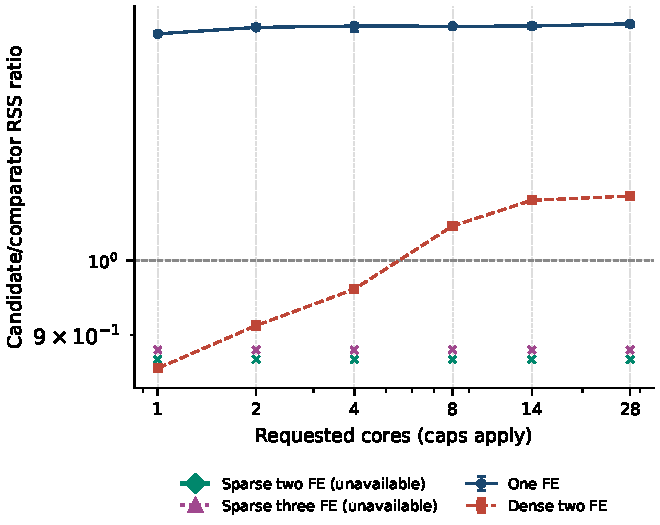
\includegraphics[width=\linewidth]{panels/ratio-ols-panels-greg-cores-peak_rss_gib.pdf}
\caption{RSS ratios by requested cores}
\end{subfigure}\par\medskip
\begin{minipage}{0.98\linewidth}\footnotesize Partial campaign. Points require all six valid warm repetitions; bars show IQR, not confidence intervals. Crosses mark missing or unvalidated points. Both axes are logarithmic. Every task reserves 28 cores; Stata-controlled computation is capped at four. OLS IID inference, ten controls. See runs.csv for exclusions. Ratios are computed within seed/node pairs. Values below one favor fereg.\end{minipage}
\end{figure}\clearpage

\begin{figure}[p]\centering
\caption{fereg/fixest: panels, maximum capacity}
\begin{subfigure}[t]{0.485\linewidth}\centering
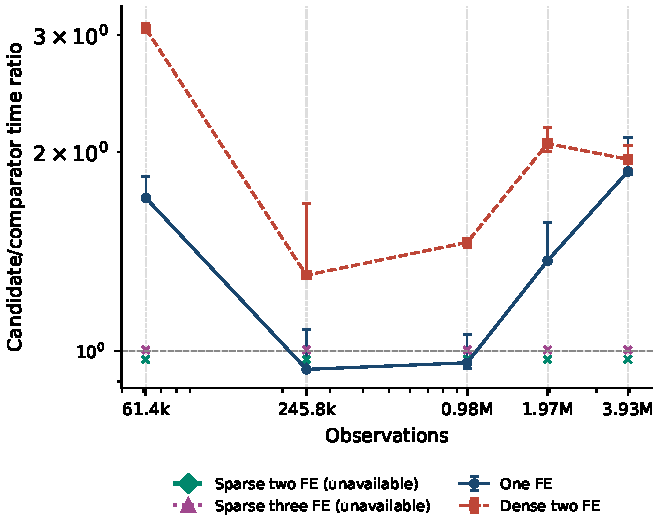
\includegraphics[width=\linewidth]{panels/ratio-ols-panels-fixest-maximum-seconds.pdf}
\caption{Time ratios by observations}
\end{subfigure}\hfill
\begin{subfigure}[t]{0.485\linewidth}\centering
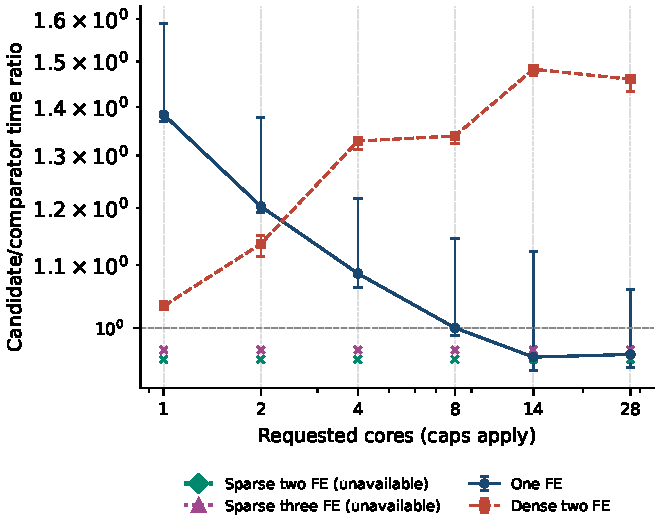
\includegraphics[width=\linewidth]{panels/ratio-ols-panels-fixest-cores-seconds.pdf}
\caption{Time ratios by requested cores}
\end{subfigure}\par\medskip
\begin{subfigure}[t]{0.485\linewidth}\centering
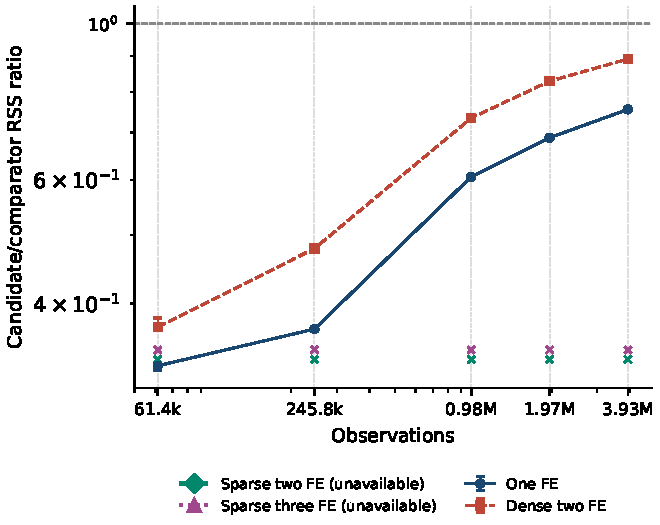
\includegraphics[width=\linewidth]{panels/ratio-ols-panels-fixest-maximum-peak_rss_gib.pdf}
\caption{RSS ratios by observations}
\end{subfigure}\hfill
\begin{subfigure}[t]{0.485\linewidth}\centering
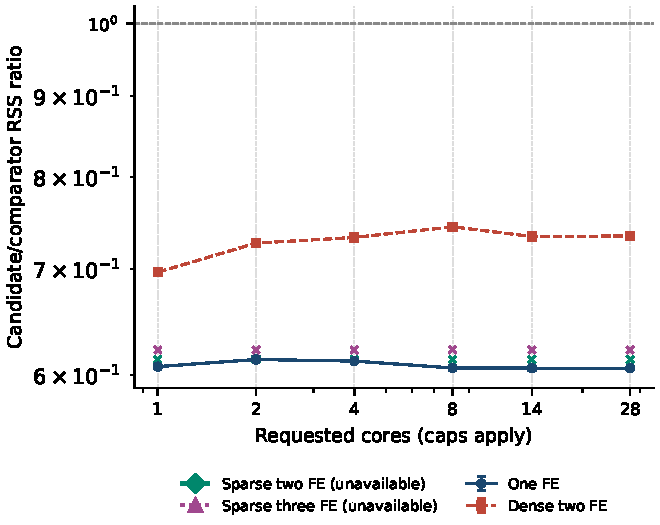
\includegraphics[width=\linewidth]{panels/ratio-ols-panels-fixest-cores-peak_rss_gib.pdf}
\caption{RSS ratios by requested cores}
\end{subfigure}\par\medskip
\begin{minipage}{0.98\linewidth}\footnotesize Partial campaign. Points require all six valid warm repetitions; bars show IQR, not confidence intervals. Crosses mark missing or unvalidated points. Both axes are logarithmic. Every task reserves 28 cores; Stata-controlled computation is capped at four. OLS IID inference, ten controls. See runs.csv for exclusions. Ratios are computed within seed/node pairs. Values below one favor fereg.\end{minipage}
\end{figure}\clearpage

\begin{figure}[p]\centering
\caption{fereg/fixest: panels, fixed capacity}
\begin{subfigure}[t]{0.485\linewidth}\centering
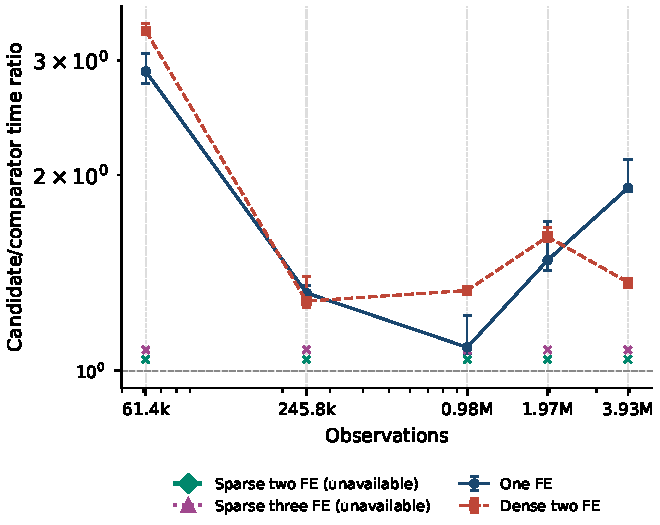
\includegraphics[width=\linewidth]{panels/ratio-ols-panels-fixest-fixed-seconds.pdf}
\caption{Time ratios by observations}
\end{subfigure}\hfill
\begin{subfigure}[t]{0.485\linewidth}\centering
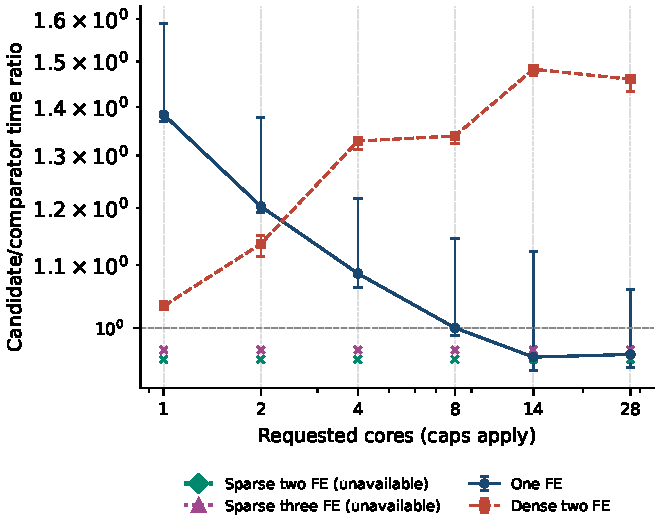
\includegraphics[width=\linewidth]{panels/ratio-ols-panels-fixest-cores-seconds.pdf}
\caption{Time ratios by requested cores}
\end{subfigure}\par\medskip
\begin{subfigure}[t]{0.485\linewidth}\centering
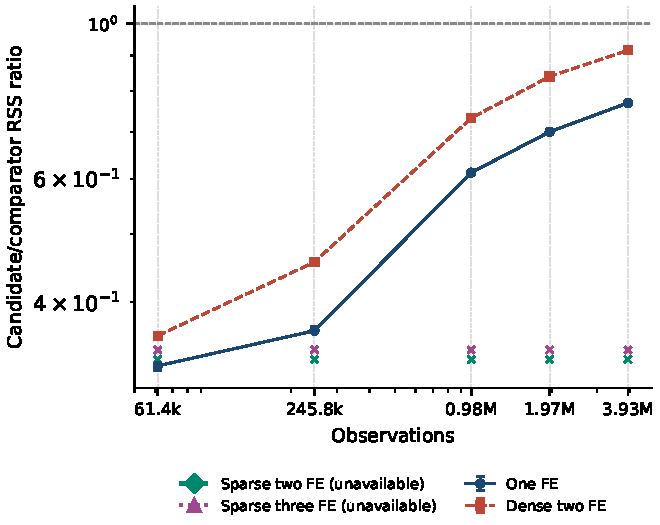
\includegraphics[width=\linewidth]{panels/ratio-ols-panels-fixest-fixed-peak_rss_gib.pdf}
\caption{RSS ratios by observations}
\end{subfigure}\hfill
\begin{subfigure}[t]{0.485\linewidth}\centering
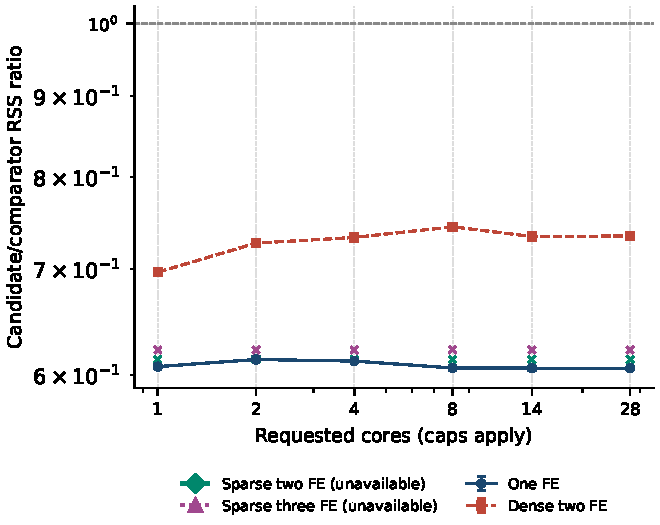
\includegraphics[width=\linewidth]{panels/ratio-ols-panels-fixest-cores-peak_rss_gib.pdf}
\caption{RSS ratios by requested cores}
\end{subfigure}\par\medskip
\begin{minipage}{0.98\linewidth}\footnotesize Partial campaign. Points require all six valid warm repetitions; bars show IQR, not confidence intervals. Crosses mark missing or unvalidated points. Both axes are logarithmic. Every task reserves 28 cores; Stata-controlled computation is capped at four. OLS IID inference, ten controls. See runs.csv for exclusions. Ratios are computed within seed/node pairs. Values below one favor fereg.\end{minipage}
\end{figure}\clearpage

\begin{figure}[p]\centering
\caption{fereg/pyfixest: panels, maximum capacity}
\begin{subfigure}[t]{0.485\linewidth}\centering
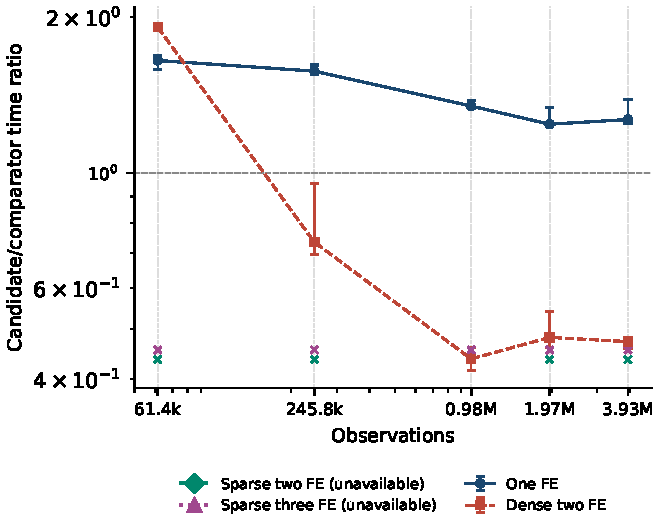
\includegraphics[width=\linewidth]{panels/ratio-ols-panels-pyfixest-maximum-seconds.pdf}
\caption{Time ratios by observations}
\end{subfigure}\hfill
\begin{subfigure}[t]{0.485\linewidth}\centering
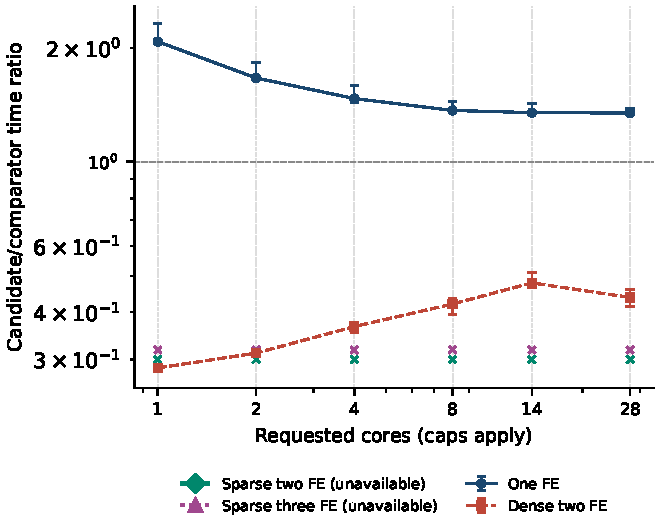
\includegraphics[width=\linewidth]{panels/ratio-ols-panels-pyfixest-cores-seconds.pdf}
\caption{Time ratios by requested cores}
\end{subfigure}\par\medskip
\begin{subfigure}[t]{0.485\linewidth}\centering
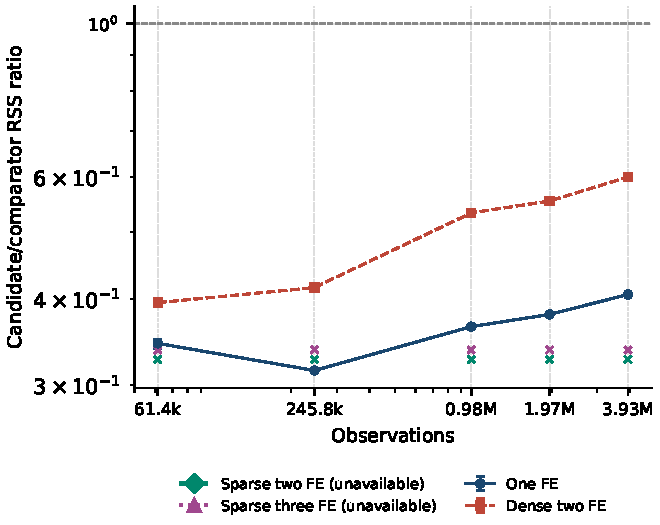
\includegraphics[width=\linewidth]{panels/ratio-ols-panels-pyfixest-maximum-peak_rss_gib.pdf}
\caption{RSS ratios by observations}
\end{subfigure}\hfill
\begin{subfigure}[t]{0.485\linewidth}\centering
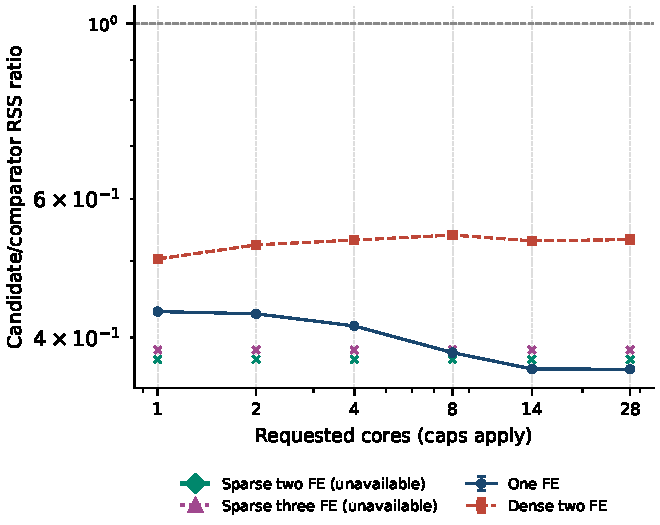
\includegraphics[width=\linewidth]{panels/ratio-ols-panels-pyfixest-cores-peak_rss_gib.pdf}
\caption{RSS ratios by requested cores}
\end{subfigure}\par\medskip
\begin{minipage}{0.98\linewidth}\footnotesize Partial campaign. Points require all six valid warm repetitions; bars show IQR, not confidence intervals. Crosses mark missing or unvalidated points. Both axes are logarithmic. Every task reserves 28 cores; Stata-controlled computation is capped at four. OLS IID inference, ten controls. See runs.csv for exclusions. Ratios are computed within seed/node pairs. Values below one favor fereg.\end{minipage}
\end{figure}\clearpage

\begin{figure}[p]\centering
\caption{fereg/pyfixest: panels, fixed capacity}
\begin{subfigure}[t]{0.485\linewidth}\centering
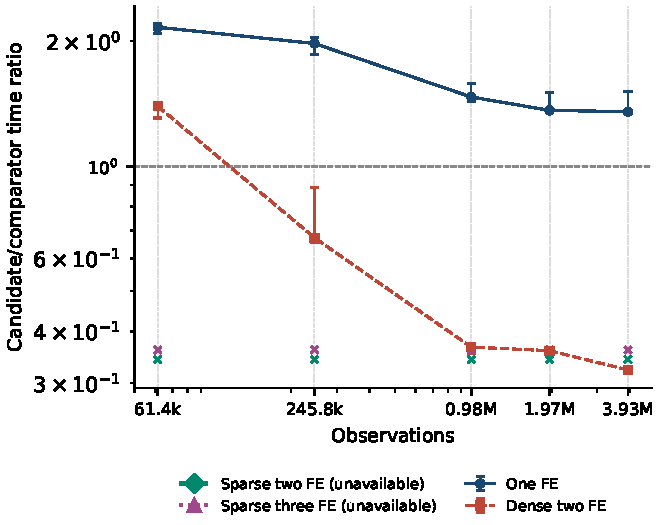
\includegraphics[width=\linewidth]{panels/ratio-ols-panels-pyfixest-fixed-seconds.pdf}
\caption{Time ratios by observations}
\end{subfigure}\hfill
\begin{subfigure}[t]{0.485\linewidth}\centering
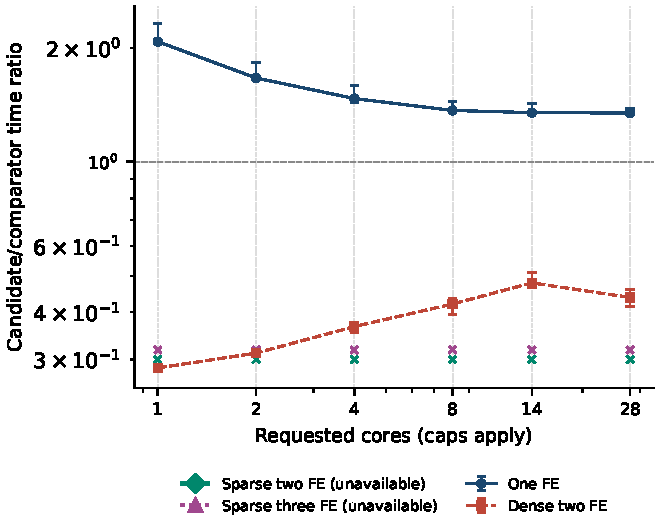
\includegraphics[width=\linewidth]{panels/ratio-ols-panels-pyfixest-cores-seconds.pdf}
\caption{Time ratios by requested cores}
\end{subfigure}\par\medskip
\begin{subfigure}[t]{0.485\linewidth}\centering
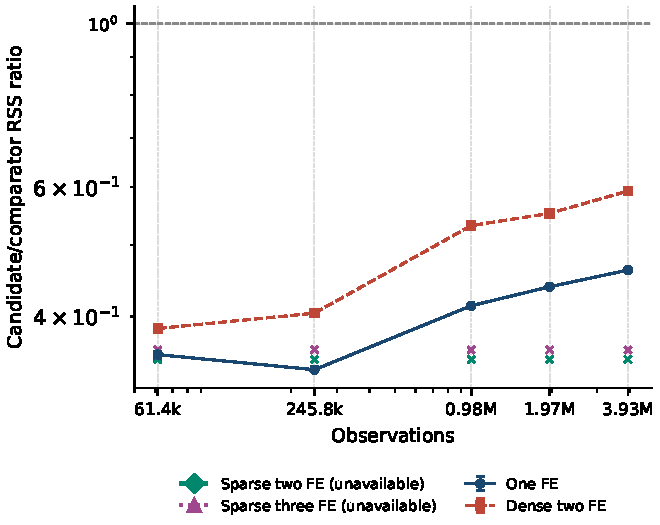
\includegraphics[width=\linewidth]{panels/ratio-ols-panels-pyfixest-fixed-peak_rss_gib.pdf}
\caption{RSS ratios by observations}
\end{subfigure}\hfill
\begin{subfigure}[t]{0.485\linewidth}\centering
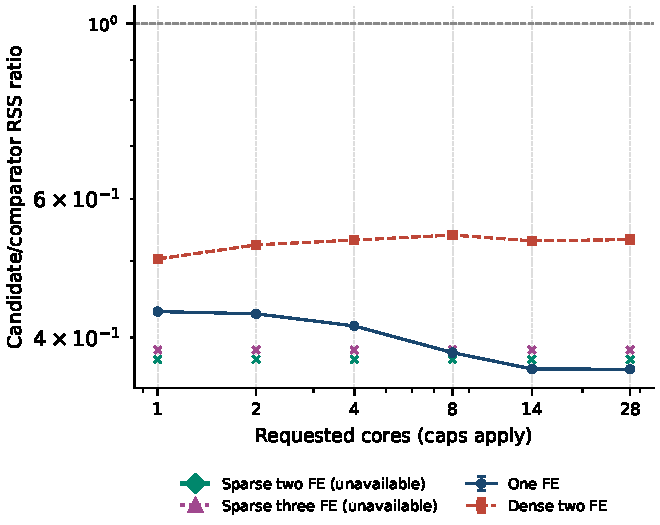
\includegraphics[width=\linewidth]{panels/ratio-ols-panels-pyfixest-cores-peak_rss_gib.pdf}
\caption{RSS ratios by requested cores}
\end{subfigure}\par\medskip
\begin{minipage}{0.98\linewidth}\footnotesize Partial campaign. Points require all six valid warm repetitions; bars show IQR, not confidence intervals. Crosses mark missing or unvalidated points. Both axes are logarithmic. Every task reserves 28 cores; Stata-controlled computation is capped at four. OLS IID inference, ten controls. See runs.csv for exclusions. Ratios are computed within seed/node pairs. Values below one favor fereg.\end{minipage}
\end{figure}\clearpage

\begin{figure}[p]\centering
\caption{fereg/reghdfe: paper, maximum capacity}
\begin{subfigure}[t]{0.485\linewidth}\centering
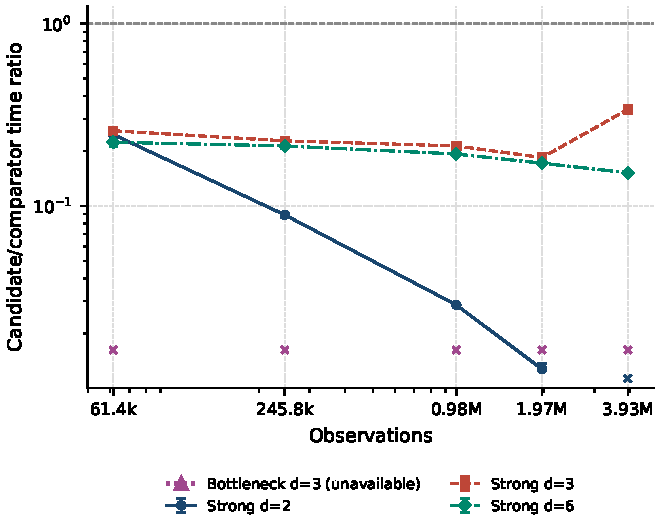
\includegraphics[width=\linewidth]{panels/ratio-ols-paper-reghdfe-maximum-seconds.pdf}
\caption{Time ratios by observations}
\end{subfigure}\hfill
\begin{subfigure}[t]{0.485\linewidth}\centering
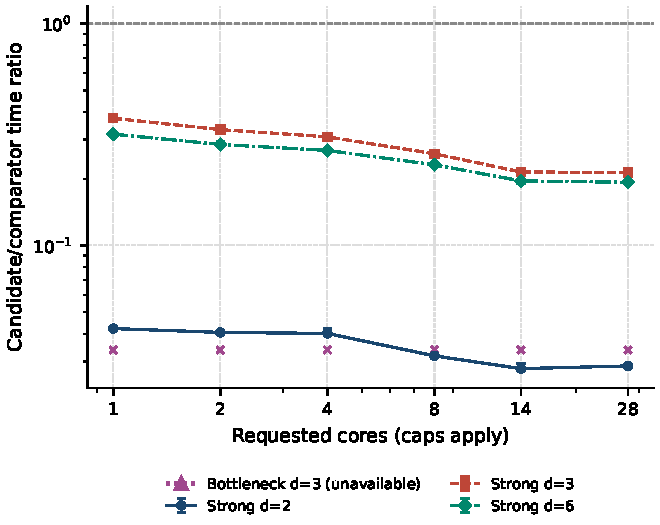
\includegraphics[width=\linewidth]{panels/ratio-ols-paper-reghdfe-cores-seconds.pdf}
\caption{Time ratios by requested cores}
\end{subfigure}\par\medskip
\begin{subfigure}[t]{0.485\linewidth}\centering
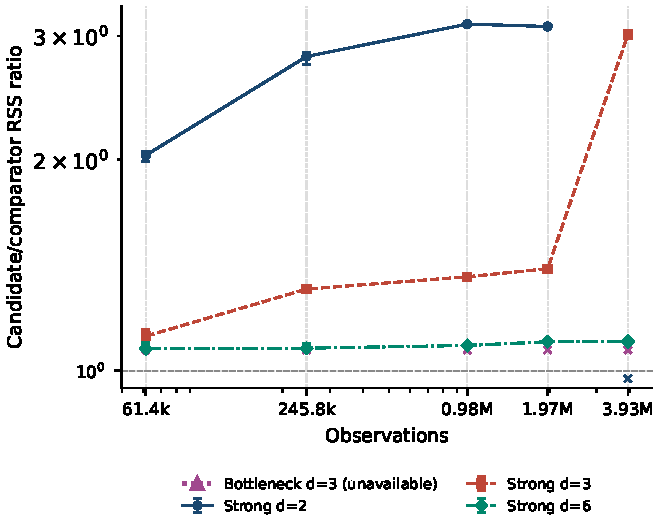
\includegraphics[width=\linewidth]{panels/ratio-ols-paper-reghdfe-maximum-peak_rss_gib.pdf}
\caption{RSS ratios by observations}
\end{subfigure}\hfill
\begin{subfigure}[t]{0.485\linewidth}\centering
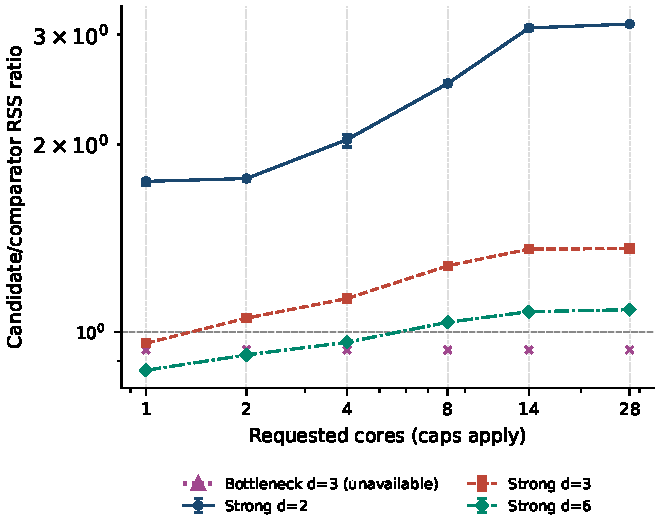
\includegraphics[width=\linewidth]{panels/ratio-ols-paper-reghdfe-cores-peak_rss_gib.pdf}
\caption{RSS ratios by requested cores}
\end{subfigure}\par\medskip
\begin{minipage}{0.98\linewidth}\footnotesize Partial campaign. Points require all six valid warm repetitions; bars show IQR, not confidence intervals. Crosses mark missing or unvalidated points. Both axes are logarithmic. Every task reserves 28 cores; Stata-controlled computation is capped at four. OLS IID inference, ten controls. See runs.csv for exclusions. Ratios are computed within seed/node pairs. Values below one favor fereg.\end{minipage}
\end{figure}\clearpage

\begin{figure}[p]\centering
\caption{fereg/reghdfe: paper, fixed capacity}
\begin{subfigure}[t]{0.485\linewidth}\centering
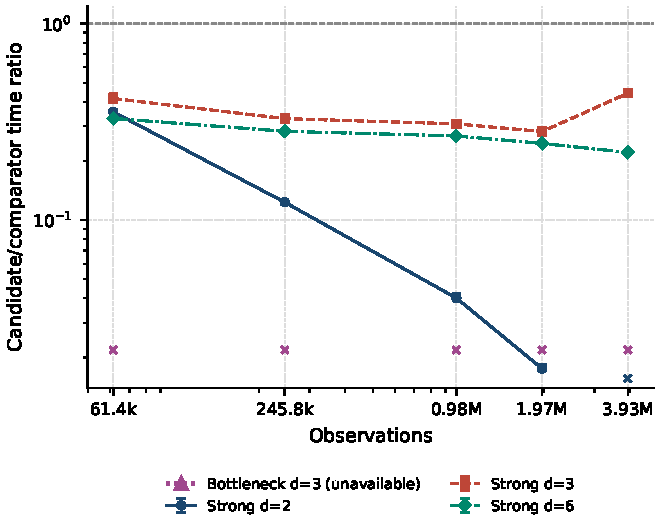
\includegraphics[width=\linewidth]{panels/ratio-ols-paper-reghdfe-fixed-seconds.pdf}
\caption{Time ratios by observations}
\end{subfigure}\hfill
\begin{subfigure}[t]{0.485\linewidth}\centering
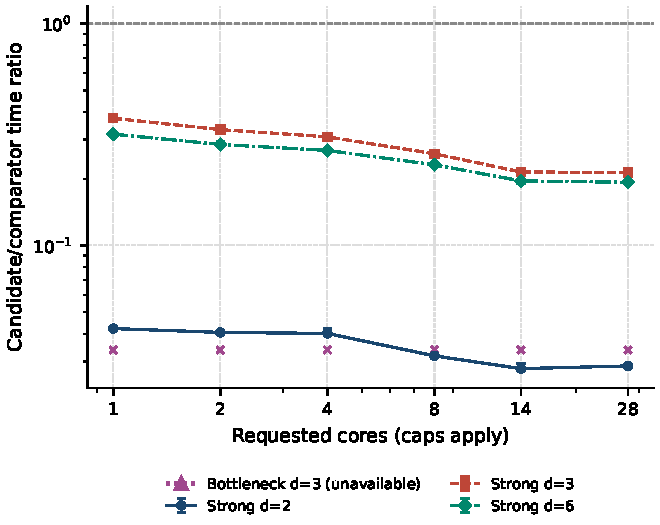
\includegraphics[width=\linewidth]{panels/ratio-ols-paper-reghdfe-cores-seconds.pdf}
\caption{Time ratios by requested cores}
\end{subfigure}\par\medskip
\begin{subfigure}[t]{0.485\linewidth}\centering
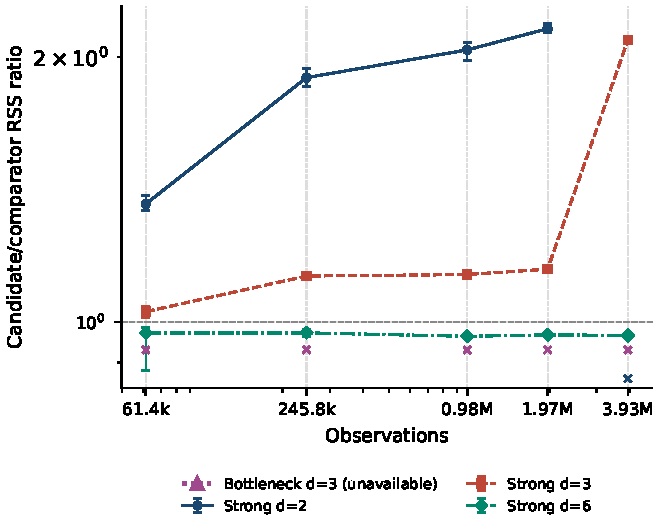
\includegraphics[width=\linewidth]{panels/ratio-ols-paper-reghdfe-fixed-peak_rss_gib.pdf}
\caption{RSS ratios by observations}
\end{subfigure}\hfill
\begin{subfigure}[t]{0.485\linewidth}\centering
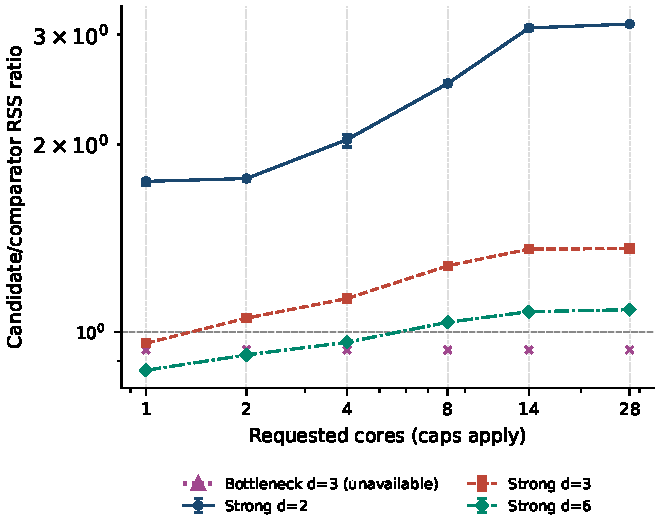
\includegraphics[width=\linewidth]{panels/ratio-ols-paper-reghdfe-cores-peak_rss_gib.pdf}
\caption{RSS ratios by requested cores}
\end{subfigure}\par\medskip
\begin{minipage}{0.98\linewidth}\footnotesize Partial campaign. Points require all six valid warm repetitions; bars show IQR, not confidence intervals. Crosses mark missing or unvalidated points. Both axes are logarithmic. Every task reserves 28 cores; Stata-controlled computation is capped at four. OLS IID inference, ten controls. See runs.csv for exclusions. Ratios are computed within seed/node pairs. Values below one favor fereg.\end{minipage}
\end{figure}\clearpage

\begin{figure}[p]\centering
\caption{fereg/areg: paper, maximum capacity}
\begin{subfigure}[t]{0.485\linewidth}\centering
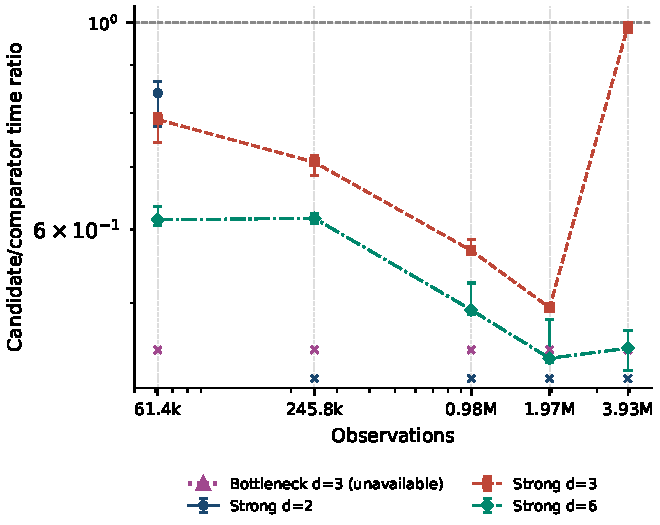
\includegraphics[width=\linewidth]{panels/ratio-ols-paper-areg-maximum-seconds.pdf}
\caption{Time ratios by observations}
\end{subfigure}\hfill
\begin{subfigure}[t]{0.485\linewidth}\centering
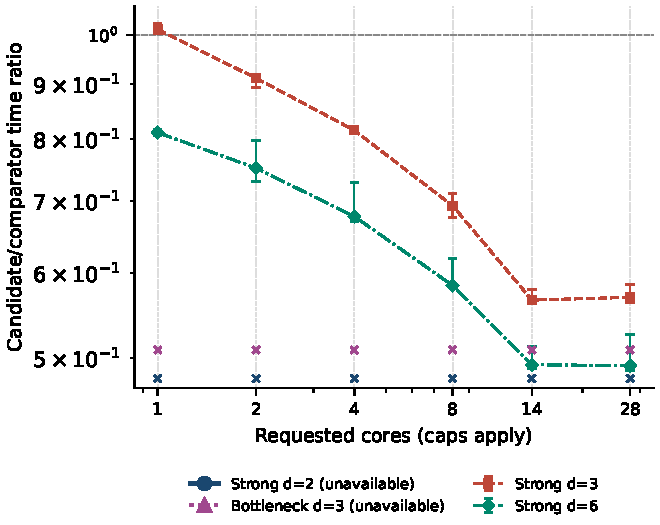
\includegraphics[width=\linewidth]{panels/ratio-ols-paper-areg-cores-seconds.pdf}
\caption{Time ratios by requested cores}
\end{subfigure}\par\medskip
\begin{subfigure}[t]{0.485\linewidth}\centering
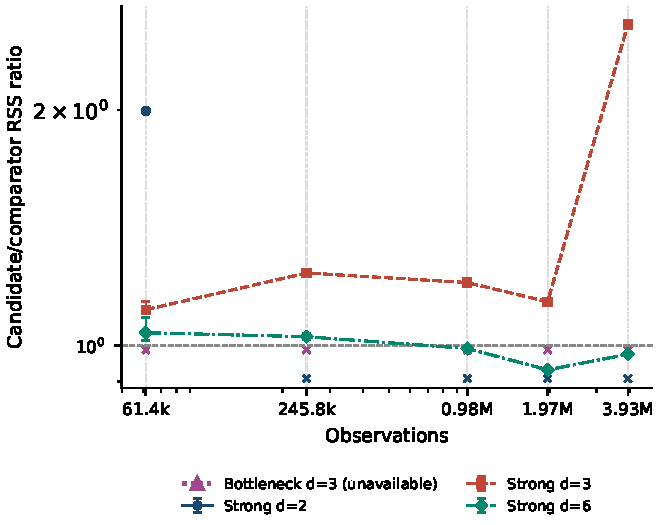
\includegraphics[width=\linewidth]{panels/ratio-ols-paper-areg-maximum-peak_rss_gib.pdf}
\caption{RSS ratios by observations}
\end{subfigure}\hfill
\begin{subfigure}[t]{0.485\linewidth}\centering
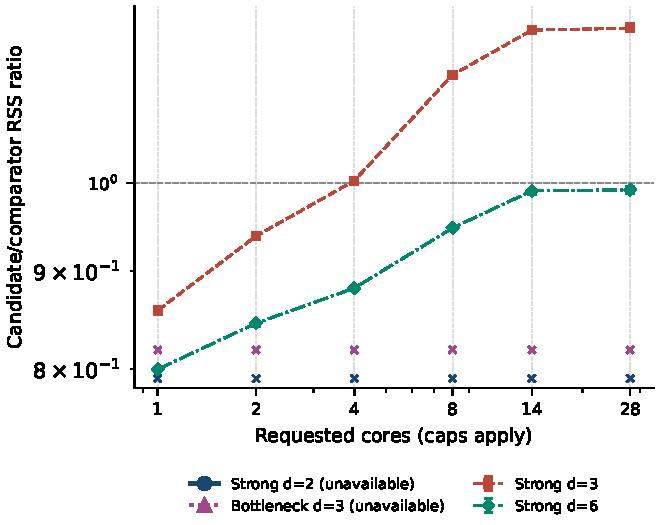
\includegraphics[width=\linewidth]{panels/ratio-ols-paper-areg-cores-peak_rss_gib.pdf}
\caption{RSS ratios by requested cores}
\end{subfigure}\par\medskip
\begin{minipage}{0.98\linewidth}\footnotesize Partial campaign. Points require all six valid warm repetitions; bars show IQR, not confidence intervals. Crosses mark missing or unvalidated points. Both axes are logarithmic. Every task reserves 28 cores; Stata-controlled computation is capped at four. OLS IID inference, ten controls. See runs.csv for exclusions. Ratios are computed within seed/node pairs. Values below one favor fereg.\end{minipage}
\end{figure}\clearpage

\begin{figure}[p]\centering
\caption{fereg/areg: paper, fixed capacity}
\begin{subfigure}[t]{0.485\linewidth}\centering
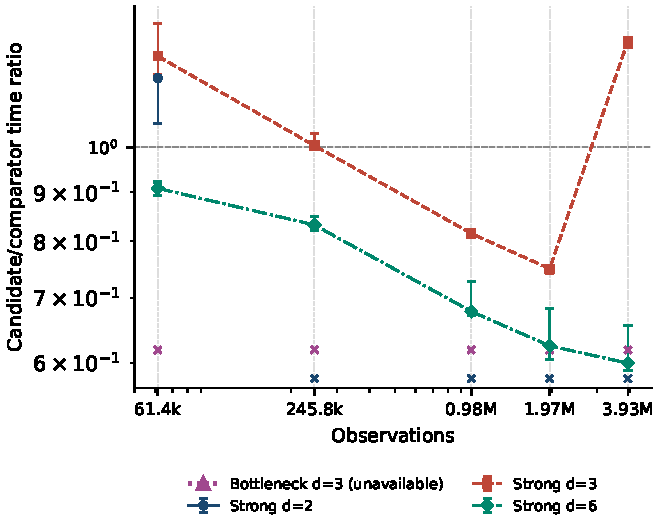
\includegraphics[width=\linewidth]{panels/ratio-ols-paper-areg-fixed-seconds.pdf}
\caption{Time ratios by observations}
\end{subfigure}\hfill
\begin{subfigure}[t]{0.485\linewidth}\centering
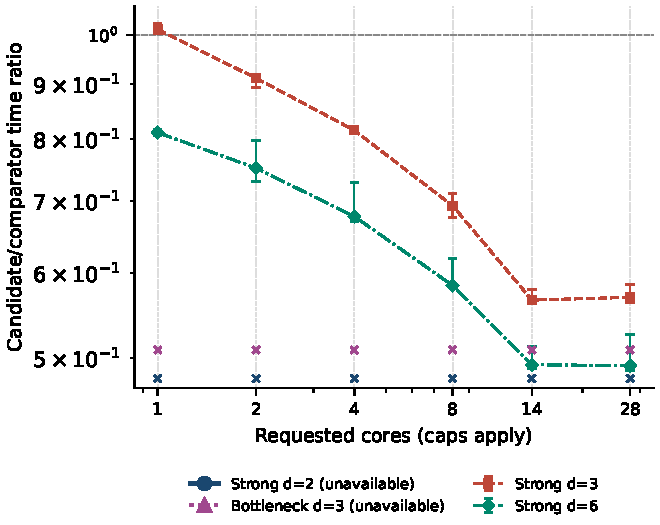
\includegraphics[width=\linewidth]{panels/ratio-ols-paper-areg-cores-seconds.pdf}
\caption{Time ratios by requested cores}
\end{subfigure}\par\medskip
\begin{subfigure}[t]{0.485\linewidth}\centering
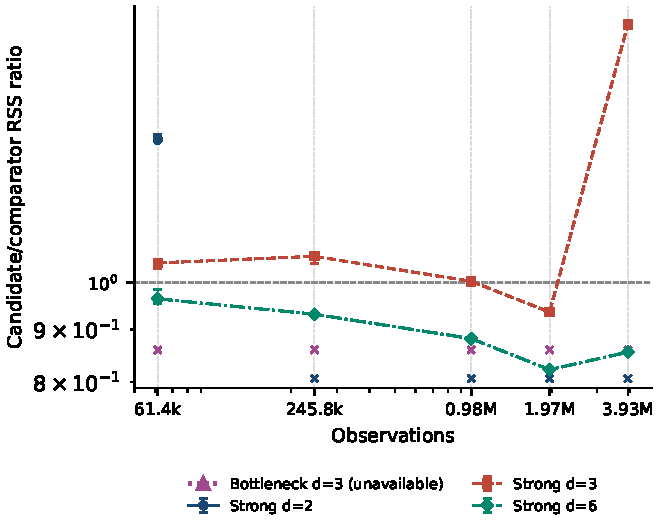
\includegraphics[width=\linewidth]{panels/ratio-ols-paper-areg-fixed-peak_rss_gib.pdf}
\caption{RSS ratios by observations}
\end{subfigure}\hfill
\begin{subfigure}[t]{0.485\linewidth}\centering
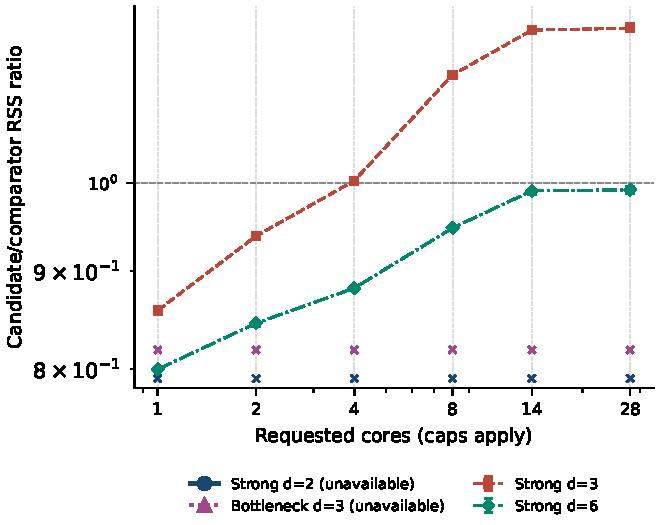
\includegraphics[width=\linewidth]{panels/ratio-ols-paper-areg-cores-peak_rss_gib.pdf}
\caption{RSS ratios by requested cores}
\end{subfigure}\par\medskip
\begin{minipage}{0.98\linewidth}\footnotesize Partial campaign. Points require all six valid warm repetitions; bars show IQR, not confidence intervals. Crosses mark missing or unvalidated points. Both axes are logarithmic. Every task reserves 28 cores; Stata-controlled computation is capped at four. OLS IID inference, ten controls. See runs.csv for exclusions. Ratios are computed within seed/node pairs. Values below one favor fereg.\end{minipage}
\end{figure}\clearpage

\begin{figure}[p]\centering
\caption{fereg/greg: paper, maximum capacity}
\begin{subfigure}[t]{0.485\linewidth}\centering
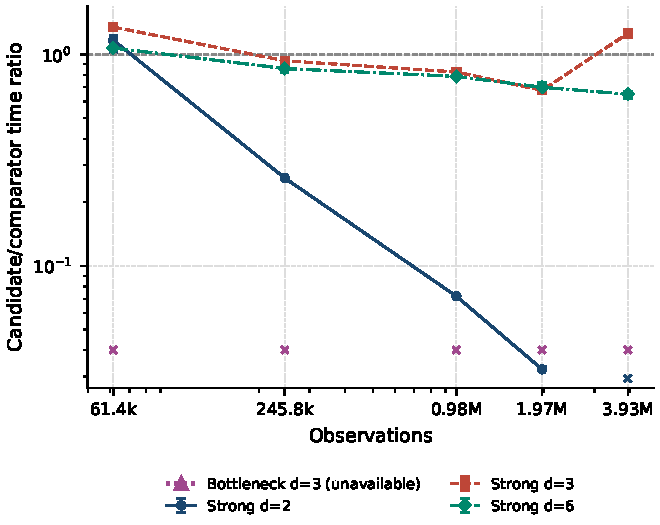
\includegraphics[width=\linewidth]{panels/ratio-ols-paper-greg-maximum-seconds.pdf}
\caption{Time ratios by observations}
\end{subfigure}\hfill
\begin{subfigure}[t]{0.485\linewidth}\centering
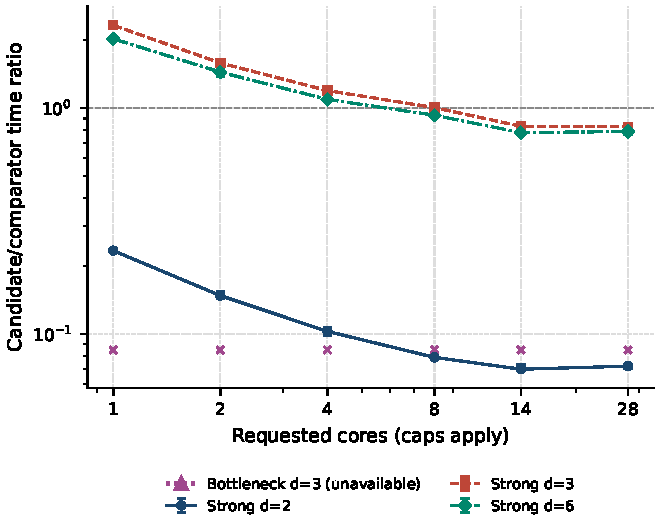
\includegraphics[width=\linewidth]{panels/ratio-ols-paper-greg-cores-seconds.pdf}
\caption{Time ratios by requested cores}
\end{subfigure}\par\medskip
\begin{subfigure}[t]{0.485\linewidth}\centering
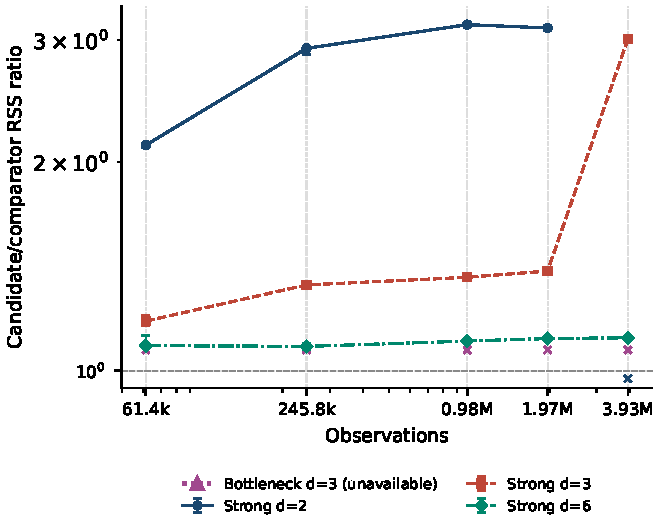
\includegraphics[width=\linewidth]{panels/ratio-ols-paper-greg-maximum-peak_rss_gib.pdf}
\caption{RSS ratios by observations}
\end{subfigure}\hfill
\begin{subfigure}[t]{0.485\linewidth}\centering
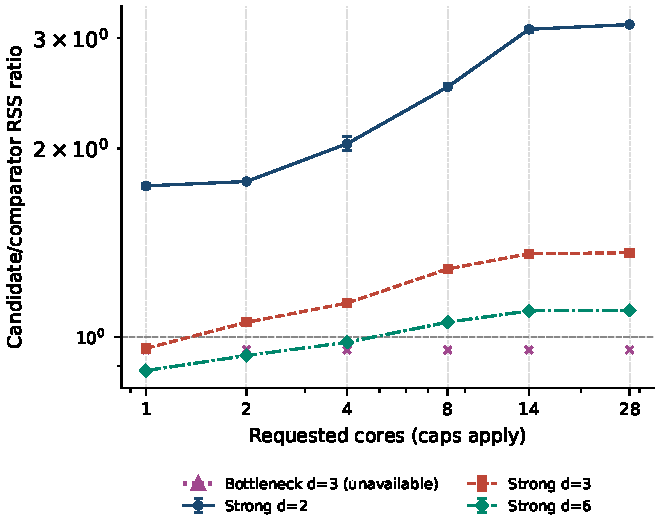
\includegraphics[width=\linewidth]{panels/ratio-ols-paper-greg-cores-peak_rss_gib.pdf}
\caption{RSS ratios by requested cores}
\end{subfigure}\par\medskip
\begin{minipage}{0.98\linewidth}\footnotesize Partial campaign. Points require all six valid warm repetitions; bars show IQR, not confidence intervals. Crosses mark missing or unvalidated points. Both axes are logarithmic. Every task reserves 28 cores; Stata-controlled computation is capped at four. OLS IID inference, ten controls. See runs.csv for exclusions. Ratios are computed within seed/node pairs. Values below one favor fereg.\end{minipage}
\end{figure}\clearpage

\begin{figure}[p]\centering
\caption{fereg/greg: paper, fixed capacity}
\begin{subfigure}[t]{0.485\linewidth}\centering
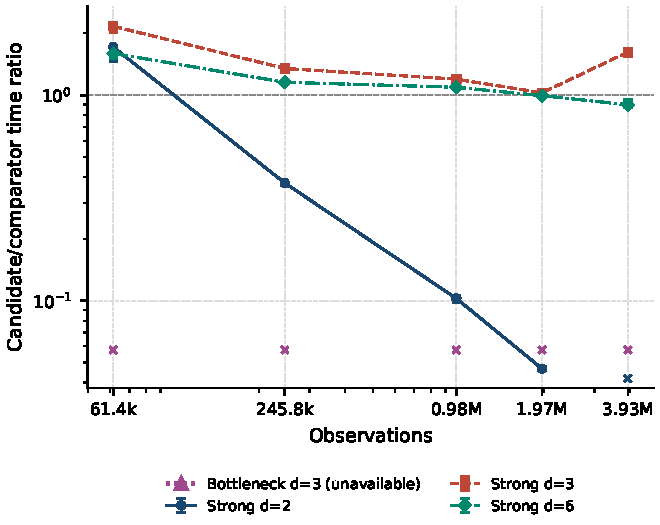
\includegraphics[width=\linewidth]{panels/ratio-ols-paper-greg-fixed-seconds.pdf}
\caption{Time ratios by observations}
\end{subfigure}\hfill
\begin{subfigure}[t]{0.485\linewidth}\centering
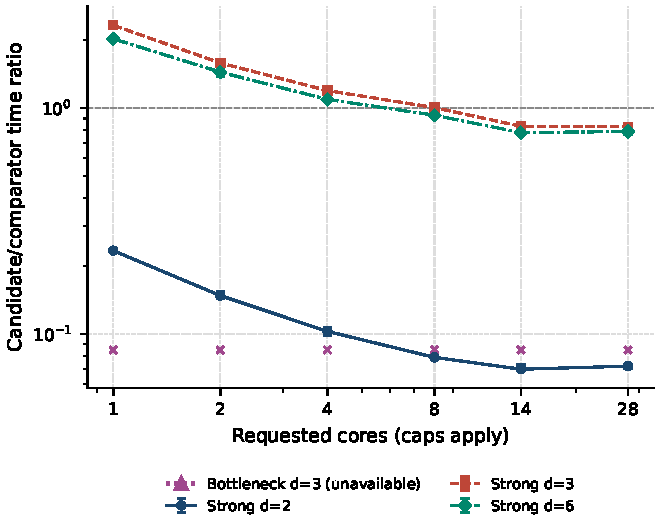
\includegraphics[width=\linewidth]{panels/ratio-ols-paper-greg-cores-seconds.pdf}
\caption{Time ratios by requested cores}
\end{subfigure}\par\medskip
\begin{subfigure}[t]{0.485\linewidth}\centering
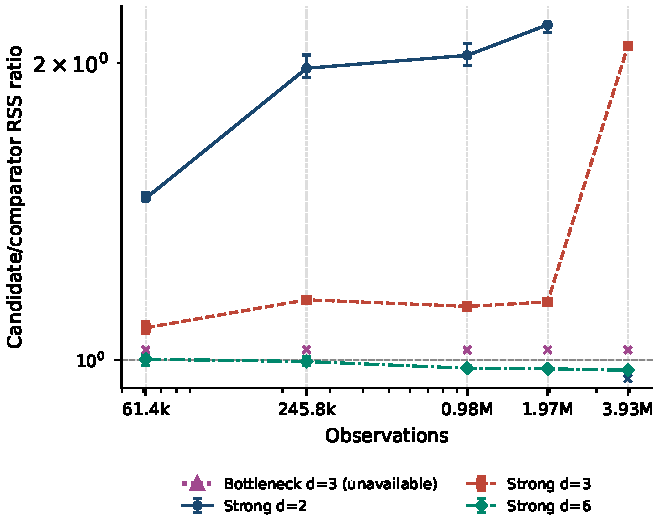
\includegraphics[width=\linewidth]{panels/ratio-ols-paper-greg-fixed-peak_rss_gib.pdf}
\caption{RSS ratios by observations}
\end{subfigure}\hfill
\begin{subfigure}[t]{0.485\linewidth}\centering
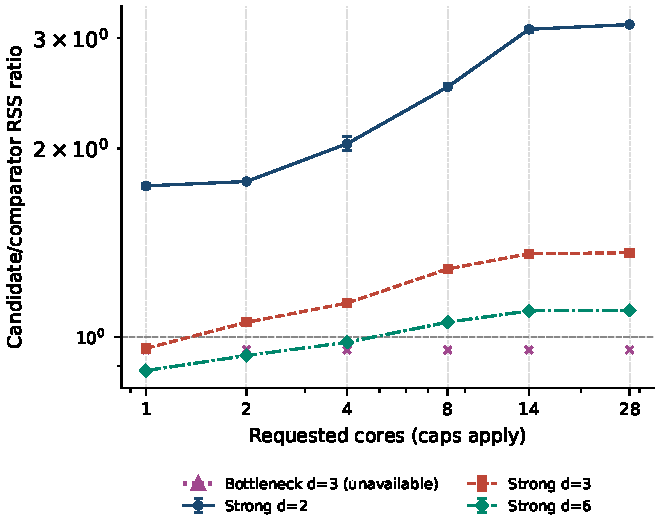
\includegraphics[width=\linewidth]{panels/ratio-ols-paper-greg-cores-peak_rss_gib.pdf}
\caption{RSS ratios by requested cores}
\end{subfigure}\par\medskip
\begin{minipage}{0.98\linewidth}\footnotesize Partial campaign. Points require all six valid warm repetitions; bars show IQR, not confidence intervals. Crosses mark missing or unvalidated points. Both axes are logarithmic. Every task reserves 28 cores; Stata-controlled computation is capped at four. OLS IID inference, ten controls. See runs.csv for exclusions. Ratios are computed within seed/node pairs. Values below one favor fereg.\end{minipage}
\end{figure}\clearpage

\begin{figure}[p]\centering
\caption{fereg/fixest: paper, maximum capacity}
\begin{subfigure}[t]{0.485\linewidth}\centering
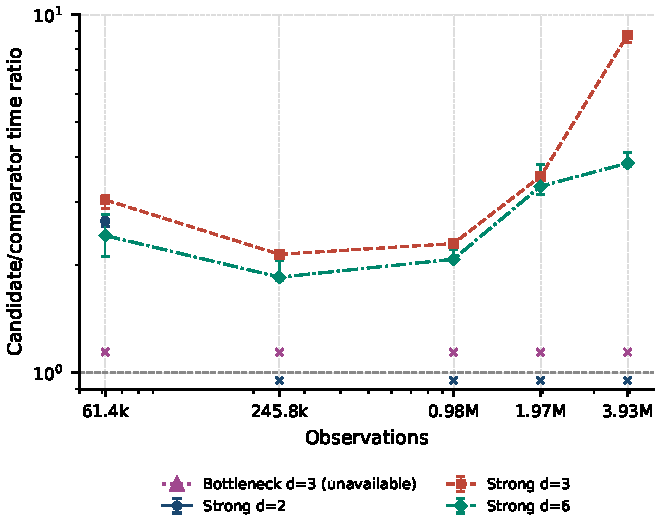
\includegraphics[width=\linewidth]{panels/ratio-ols-paper-fixest-maximum-seconds.pdf}
\caption{Time ratios by observations}
\end{subfigure}\hfill
\begin{subfigure}[t]{0.485\linewidth}\centering
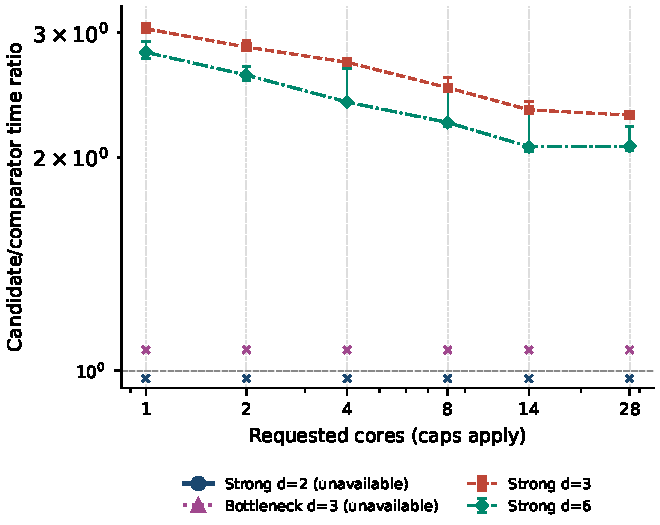
\includegraphics[width=\linewidth]{panels/ratio-ols-paper-fixest-cores-seconds.pdf}
\caption{Time ratios by requested cores}
\end{subfigure}\par\medskip
\begin{subfigure}[t]{0.485\linewidth}\centering
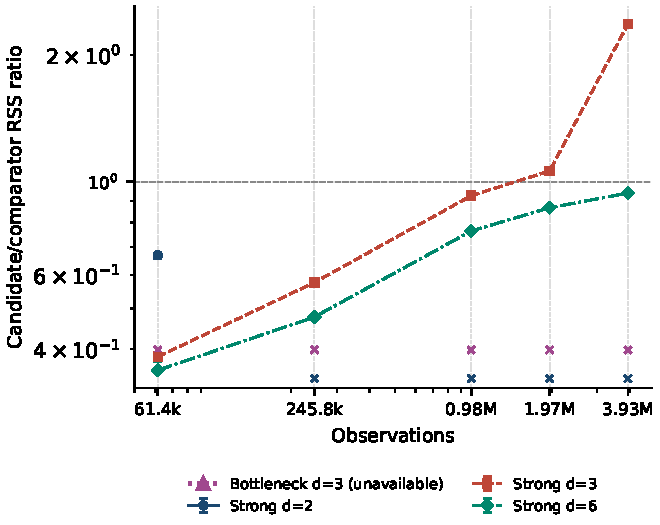
\includegraphics[width=\linewidth]{panels/ratio-ols-paper-fixest-maximum-peak_rss_gib.pdf}
\caption{RSS ratios by observations}
\end{subfigure}\hfill
\begin{subfigure}[t]{0.485\linewidth}\centering
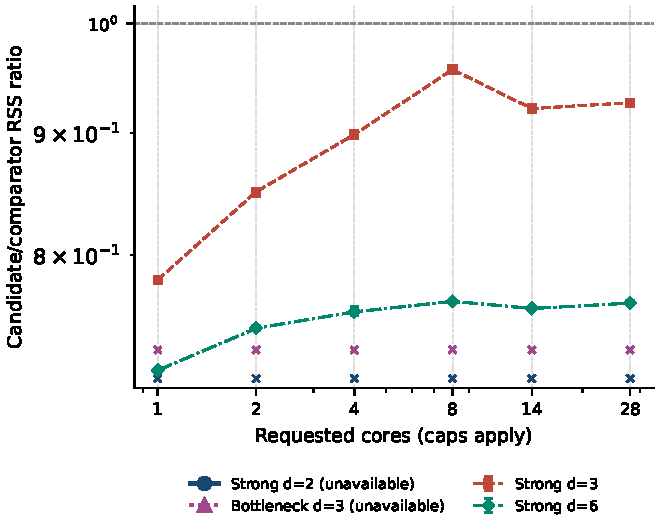
\includegraphics[width=\linewidth]{panels/ratio-ols-paper-fixest-cores-peak_rss_gib.pdf}
\caption{RSS ratios by requested cores}
\end{subfigure}\par\medskip
\begin{minipage}{0.98\linewidth}\footnotesize Partial campaign. Points require all six valid warm repetitions; bars show IQR, not confidence intervals. Crosses mark missing or unvalidated points. Both axes are logarithmic. Every task reserves 28 cores; Stata-controlled computation is capped at four. OLS IID inference, ten controls. See runs.csv for exclusions. Ratios are computed within seed/node pairs. Values below one favor fereg.\end{minipage}
\end{figure}\clearpage

\begin{figure}[p]\centering
\caption{fereg/fixest: paper, fixed capacity}
\begin{subfigure}[t]{0.485\linewidth}\centering
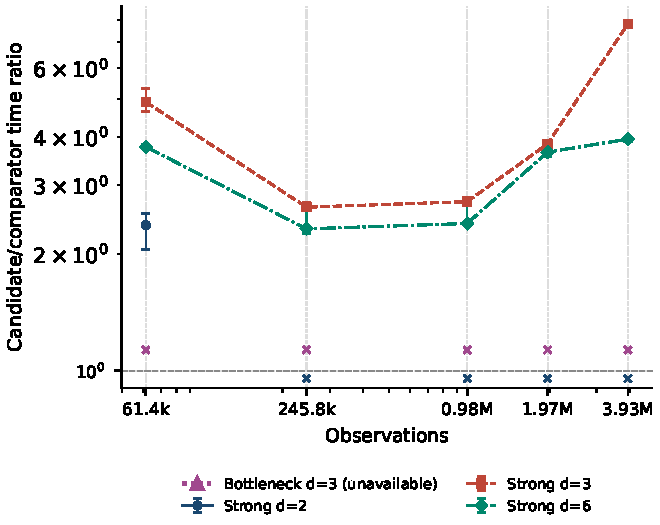
\includegraphics[width=\linewidth]{panels/ratio-ols-paper-fixest-fixed-seconds.pdf}
\caption{Time ratios by observations}
\end{subfigure}\hfill
\begin{subfigure}[t]{0.485\linewidth}\centering
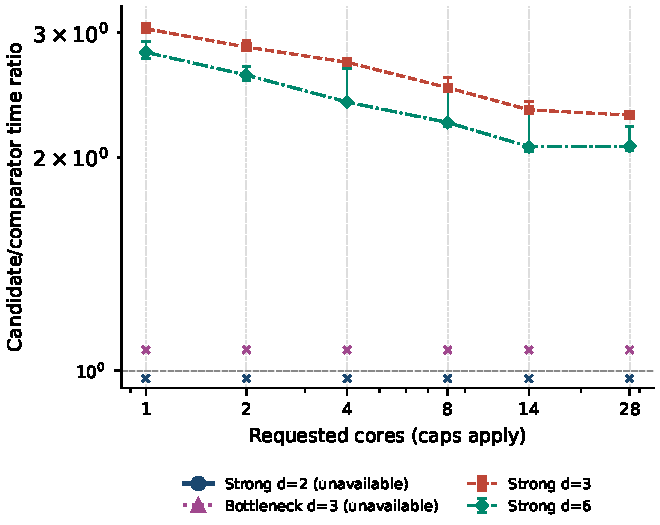
\includegraphics[width=\linewidth]{panels/ratio-ols-paper-fixest-cores-seconds.pdf}
\caption{Time ratios by requested cores}
\end{subfigure}\par\medskip
\begin{subfigure}[t]{0.485\linewidth}\centering
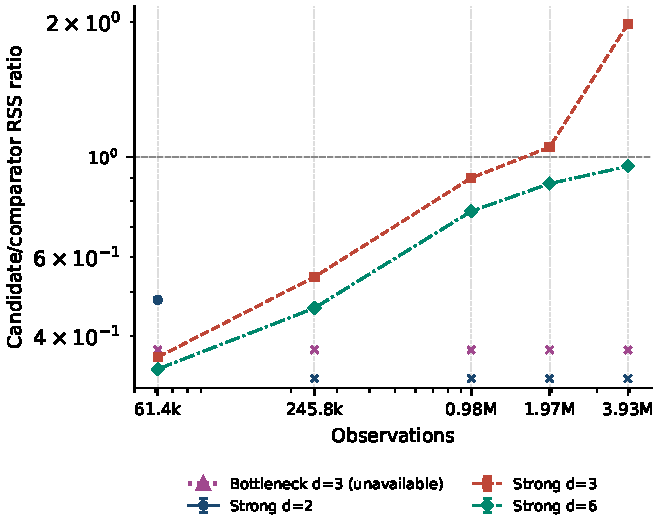
\includegraphics[width=\linewidth]{panels/ratio-ols-paper-fixest-fixed-peak_rss_gib.pdf}
\caption{RSS ratios by observations}
\end{subfigure}\hfill
\begin{subfigure}[t]{0.485\linewidth}\centering
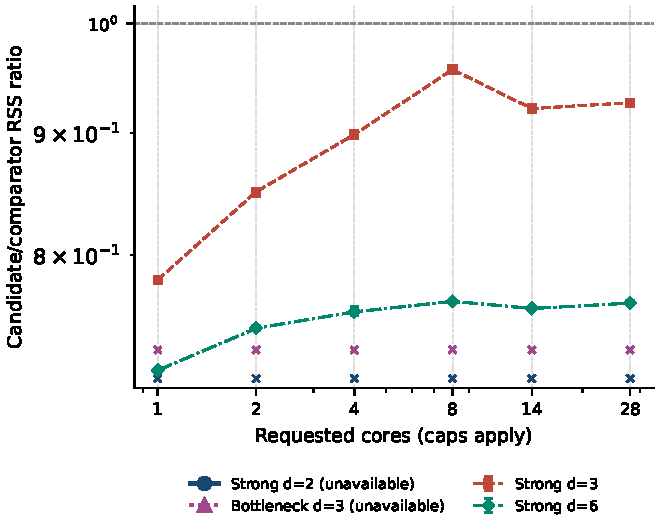
\includegraphics[width=\linewidth]{panels/ratio-ols-paper-fixest-cores-peak_rss_gib.pdf}
\caption{RSS ratios by requested cores}
\end{subfigure}\par\medskip
\begin{minipage}{0.98\linewidth}\footnotesize Partial campaign. Points require all six valid warm repetitions; bars show IQR, not confidence intervals. Crosses mark missing or unvalidated points. Both axes are logarithmic. Every task reserves 28 cores; Stata-controlled computation is capped at four. OLS IID inference, ten controls. See runs.csv for exclusions. Ratios are computed within seed/node pairs. Values below one favor fereg.\end{minipage}
\end{figure}\clearpage

\begin{figure}[p]\centering
\caption{fereg/pyfixest: paper, maximum capacity}
\begin{subfigure}[t]{0.485\linewidth}\centering
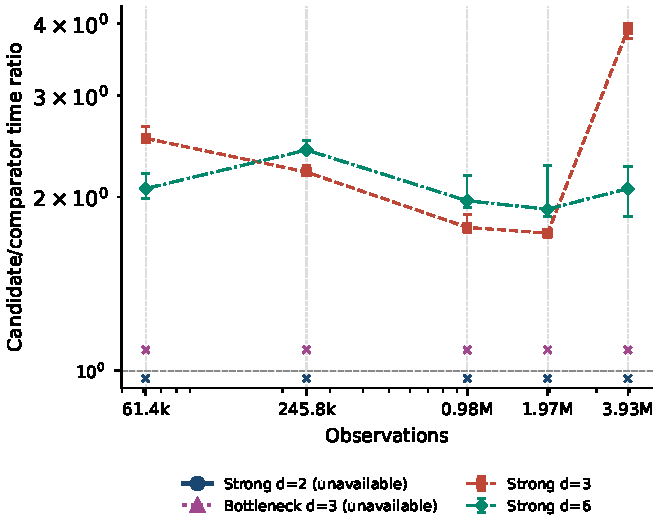
\includegraphics[width=\linewidth]{panels/ratio-ols-paper-pyfixest-maximum-seconds.pdf}
\caption{Time ratios by observations}
\end{subfigure}\hfill
\begin{subfigure}[t]{0.485\linewidth}\centering
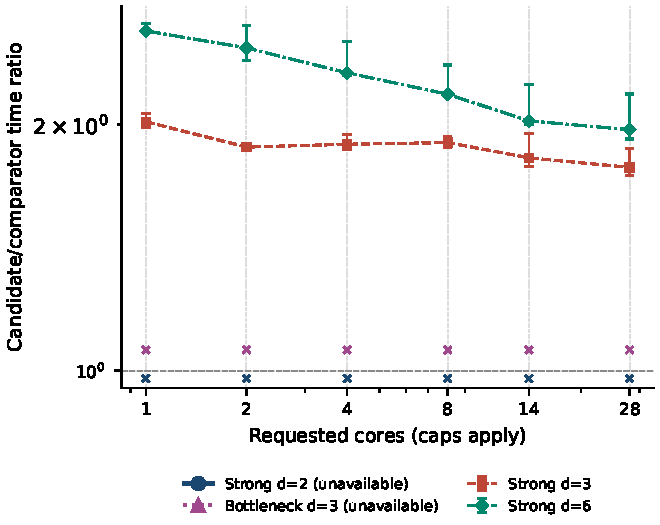
\includegraphics[width=\linewidth]{panels/ratio-ols-paper-pyfixest-cores-seconds.pdf}
\caption{Time ratios by requested cores}
\end{subfigure}\par\medskip
\begin{subfigure}[t]{0.485\linewidth}\centering
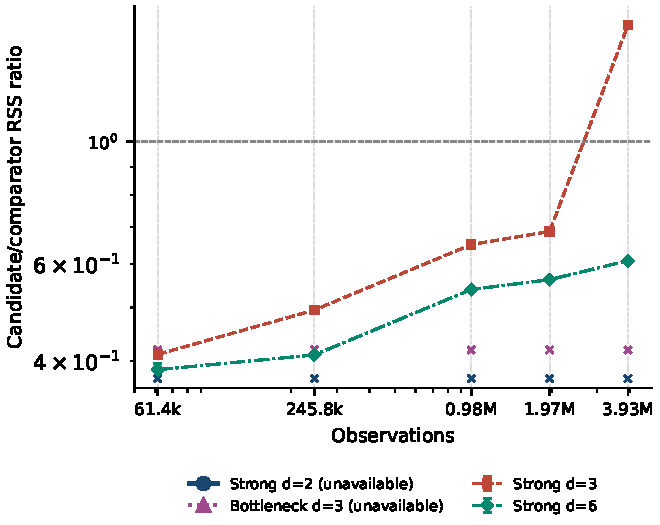
\includegraphics[width=\linewidth]{panels/ratio-ols-paper-pyfixest-maximum-peak_rss_gib.pdf}
\caption{RSS ratios by observations}
\end{subfigure}\hfill
\begin{subfigure}[t]{0.485\linewidth}\centering
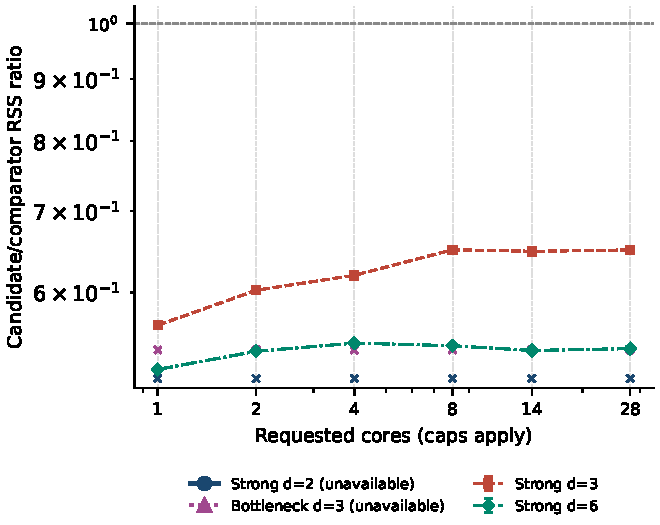
\includegraphics[width=\linewidth]{panels/ratio-ols-paper-pyfixest-cores-peak_rss_gib.pdf}
\caption{RSS ratios by requested cores}
\end{subfigure}\par\medskip
\begin{minipage}{0.98\linewidth}\footnotesize Partial campaign. Points require all six valid warm repetitions; bars show IQR, not confidence intervals. Crosses mark missing or unvalidated points. Both axes are logarithmic. Every task reserves 28 cores; Stata-controlled computation is capped at four. OLS IID inference, ten controls. See runs.csv for exclusions. Ratios are computed within seed/node pairs. Values below one favor fereg.\end{minipage}
\end{figure}\clearpage

\begin{figure}[p]\centering
\caption{fereg/pyfixest: paper, fixed capacity}
\begin{subfigure}[t]{0.485\linewidth}\centering
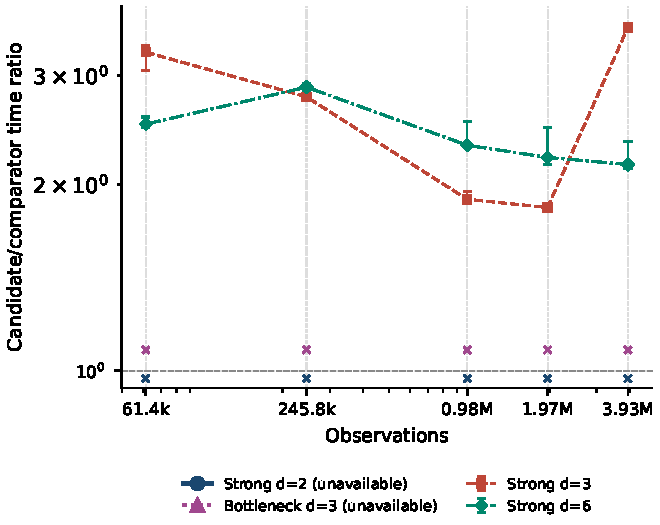
\includegraphics[width=\linewidth]{panels/ratio-ols-paper-pyfixest-fixed-seconds.pdf}
\caption{Time ratios by observations}
\end{subfigure}\hfill
\begin{subfigure}[t]{0.485\linewidth}\centering
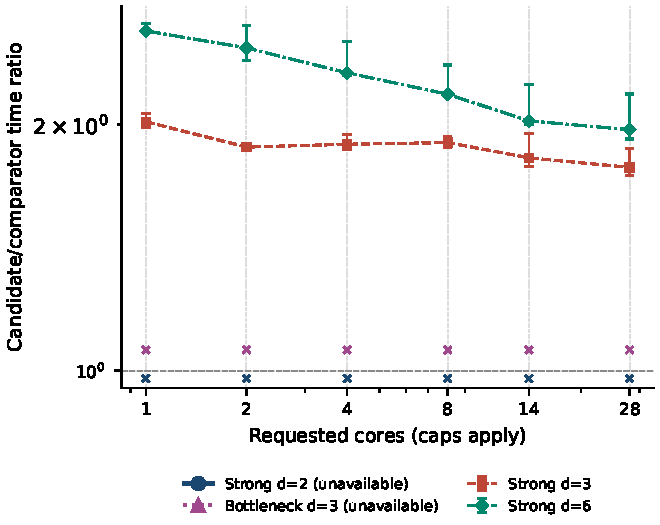
\includegraphics[width=\linewidth]{panels/ratio-ols-paper-pyfixest-cores-seconds.pdf}
\caption{Time ratios by requested cores}
\end{subfigure}\par\medskip
\begin{subfigure}[t]{0.485\linewidth}\centering
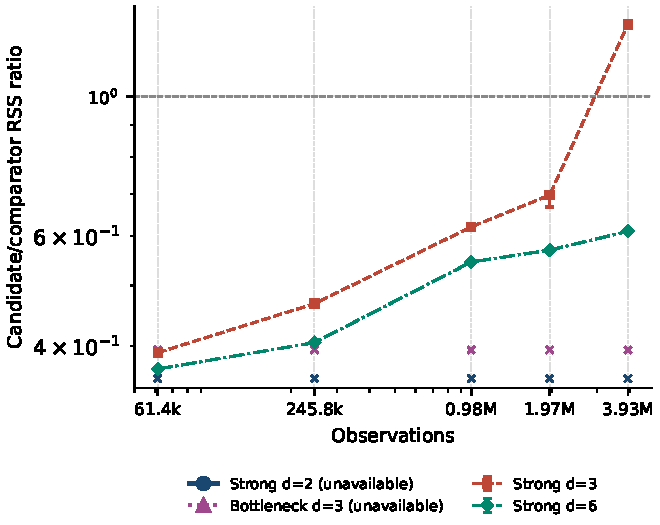
\includegraphics[width=\linewidth]{panels/ratio-ols-paper-pyfixest-fixed-peak_rss_gib.pdf}
\caption{RSS ratios by observations}
\end{subfigure}\hfill
\begin{subfigure}[t]{0.485\linewidth}\centering
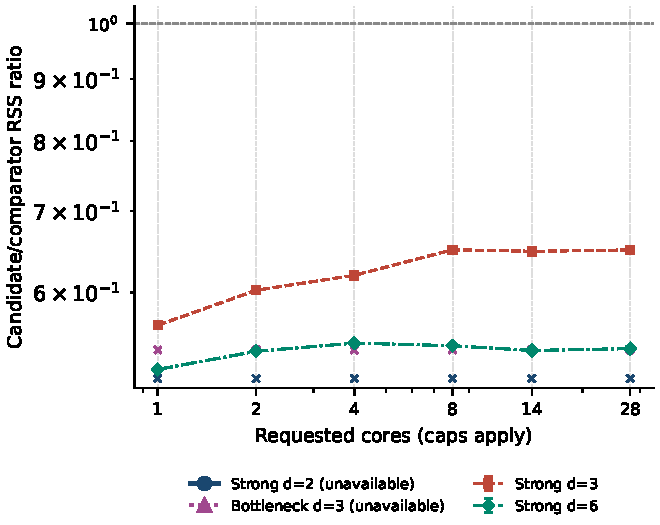
\includegraphics[width=\linewidth]{panels/ratio-ols-paper-pyfixest-cores-peak_rss_gib.pdf}
\caption{RSS ratios by requested cores}
\end{subfigure}\par\medskip
\begin{minipage}{0.98\linewidth}\footnotesize Partial campaign. Points require all six valid warm repetitions; bars show IQR, not confidence intervals. Crosses mark missing or unvalidated points. Both axes are logarithmic. Every task reserves 28 cores; Stata-controlled computation is capped at four. OLS IID inference, ten controls. See runs.csv for exclusions. Ratios are computed within seed/node pairs. Values below one favor fereg.\end{minipage}
\end{figure}\clearpage

\end{document}
